\chapter{伴随、极限与余极限 II}\label{ch:adjunctions-limits-colimits-II}


在第 2 章中，我们在某个\trInfinityCosmos{}的、由诸\trInfinityCategory{}、%
\trFunctor{}与\trNaturalTransformation{}组成的\trHomotopyTwoCategory{}中，%
以绝对\trLifting{}图刻画这些概念，由此发展了\trInfinityCategory{}之间的%
\trAdjunction{}以及取值于\trInfinityCategory{}的\trDiagram{}之\trLimit{}与%
\trColimit{}的基本理论。
绝对\trLifting{}图虽然便于证明关乎\trAdjunction{}、\trLimit{}与\trColimit{}的%
诸定理，却并不明显地表达出与这些概念相联系的熟知的\trUniversalProperty。%
在本章中，我们以第 3 章的\trCommaInfinityCategory{}为载体，对这些%
\trUniversalProperty{}给出精确的表述，并证明：关于\trAdjunction{}、%
\trLimit{}与\trColimit{}的新刻画等价于先前的定义。事实上，本章的许多%
主要结果只不过是刻画可表示\trCommaInfinityCategory{}的那些一般定理的%
特例而已。

利用\trCommaInfinityCategory{}理论，我们在 4.1 节中快速证明一系列刻画%
\trAdjunction{}之\trUniversalProperty{}的结果。特别地，第 3 章中的%
定理 3.5.8 在命题 4.1.1 中特殊化，借助一个「转置等价」刻画了函子%
$f\colon B\to A$ 与 $u\colon A\to B$ 的伴随对：
\[
  \mathrm{Hom}_A(f,A)\simeq_{A\times B}\mathrm{Hom}_B(B,u),
\]
而第 3 章中的推论 3.6.10 在命题 4.1.6 中特殊化，给出了一个判据，它保证%
给定\trFunctor{}的\trLeftAdjoint{}或\trRightAdjoint{}存在。

在 4.2 节的一段插曲中，我们把图表之上或之下的%
\emph{\trInfinityCategoryOfCones}作为一个\trCommaInfinityCategory{}引入。%
当诸\trDiagram{}的标号形状由一个\trSimplicialSet{}给出时，还可以从 Joyal%
的\trJoin（join）与切片（slice）构造出发，建立一个等价的模型。
图表之上或之下的诸\trInfinityCategoryOfCones{}将在 4.3 节中对\trLimit{}与%
\trColimit{}之\trUniversalProperty{}的研究中占有突出地位。在那里我们将看到，%
第 3 章中的定理 3.5.8 经特殊化即证得命题 4.3.1——它把一个\trDiagram{}的%
\trLimit{}刻画为%
\trInfinityCategoryOfCones{}的一个右表示；而第 3 章中的推论 3.6.10 在%
命题 4.3.2 中特殊化，把一个\trLimit\trCone{}刻画为该%
\trInfinityCategoryOfCones{}中的一个\trTerminal{}元素。

由于本章诸主要结果的证明都出现在第 3 章中——在那里它们在一个更一般的%
框架下得到发展——我们在这里得以把精力集中于应用。在 4.4 节中，我们引入%
\emph{\trPointed{}∞-范畴}——此类∞-范畴拥有一个既是\trInitial{}元素又是%
\trTerminal{}元素的零\trElement{}——并展示如何用它来构造%
「\trLoops$\dashv$\trSuspension{}」伴随。
拥有\trFiber{}序列与余\trFiber{}序列（这两类序列定义出同一个%
\emph{正合三角}族）的\trPointed{}∞-范畴称为\emph{\trStable}。在探索%
\trStable{}∞-范畴的性质的过程中，我们会遇到若干彼此等价的刻画，它们%
列举于定理 4.4.12 中。

刻画\trAdjunction{}、\trLimit{}与\trColimit{}的那些\trFiberedEquivalence{}，%
可以理解为 Eilenberg 与 Mac Lane 的著名自然等价 $[42]$ 的∞-范畴论类比。%
为表述这种「自然性」，我们观察到：基底∞-范畴中的箭头，以协变的函子性%
方式作用于与一个\trCommaInfinityCategory{}相关联的余定义域投影函子的诸%
\trFiber{}，并以反变的函子性方式作用于其定义域投影函子的诸\trFiber{}。%
这是第 5 章的主题。

\providecommand{\qcOne}{\mathbf{1}}   %
\providecommand{\qcor}[1]{\ulcorner#1\urcorner}   %

\section{伴随的\trUniversalProperty}\label{sec:universal-property-of-adjunctions}

一对对立的\trFunctor{}之间的\trAdjunction{}，同样可以由二者作为%
\trCommaInfinityCategory{}的左表示与右表示之间的一个「转置等价」来编码。

\begin{proposition}[作为\trFiberedEquivalence{}的\trAdjunction]\label{prop:adjunction-as-fibered-equivalence}
一对对立的\trFunctor{} $u\colon A\to B$ 与 $f\colon B\to A$ 构成一个%
\trAdjunction{} $f\dashv u$，当且仅当
$\mathrm{Hom}_A(f,A)\simeq_{A\times B}\mathrm{Hom}_B(B,u)$。
\end{proposition}

这是定理 3.5.8 的一个特例，故本无需进一步论证；但我们仍然给出一个简短的%
证明，以温习 3.5 节中证明过的那些结果。

\begin{proof}
若 $f\dashv u$，则由引理 2.3.7，其\trCounit{}
$\epsilon\colon fu\Rightarrow\mathrm{id}_A$ 定义了一个绝对右\trLifting{}图。
据定理 3.5.8，左侧的粘贴复合
\begin{center}
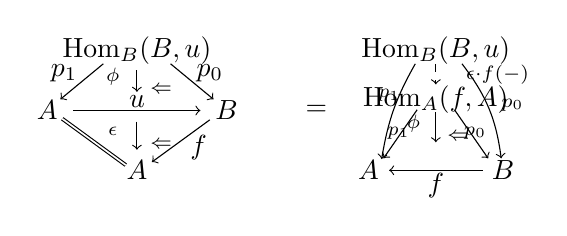
\begin{tikzpicture}[x=1.35em,y=1.35em]
  \node (H1) at (1.8,3.2) {$\mathrm{Hom}_B(B,u)$};
  \node (A2) at (-0.6,1.6) {$A$};
  \node (B2) at (4.2,1.6) {$B$};
  \node (A3) at (1.8,0) {$A$};
  \draw[->] (0.9,2.85) -- (-0.25,1.9);
  \node at (-0.15,2.6) {$p_1$};
  \draw[->] (2.7,2.85) -- (3.85,1.9);
  \node at (3.75,2.6) {$p_0$};
  \draw[->] (1.8,2.68) -- (1.8,2.1);
  \node at (1.15,2.5) {$\scriptstyle\phi$};
  \node at (2.45,2.15) {$\scriptstyle\Leftarrow$};
  \draw[->] (0.1,1.6) -- (3.5,1.6);
  \node at (1.8,1.85) {$u$};
  \draw[double] (-0.2,1.38) -- (1.5,0.14);
  \draw[->] (3.75,1.35) -- (2.2,0.22);
  \node at (3.45,0.6) {$f$};
  \draw[->] (1.8,1.3) -- (1.8,0.55);
  \node at (1.15,1.05) {$\scriptstyle\epsilon$};
  \node at (2.45,0.68) {$\scriptstyle\Leftarrow$};
  \node at (6.6,1.6) {$=$};
  \node (H2) at (9.8,3.2) {$\mathrm{Hom}_B(B,u)$};
  \node (M2) at (9.8,1.9) {$\mathrm{Hom}_A(f,A)$};
  \node (A4) at (8.0,0) {$A$};
  \node (B4) at (11.6,0) {$B$};
  \draw[->,dashed] (9.8,2.85) -- (9.8,2.3);
  \node at (11.45,2.55) {$\scriptstyle\qcor{\epsilon\cdot f(-)}$};
  \draw[->] (9.25,2.85) to[bend right=10] (8.35,0.3);
  \node at (8.55,2.0) {$\scriptstyle p_1$};
  \draw[->] (10.5,2.85) to[bend left=15] (11.55,0.32);
  \node at (11.85,1.75) {$\scriptstyle p_0$};
  \draw[->] (9.3,1.62) -- (8.4,0.32);
  \node at (8.8,1.0) {$\scriptstyle p_1$};
  \draw[->] (10.3,1.62) -- (11.2,0.32);
  \node at (10.85,1.0) {$\scriptstyle p_0$};
  \draw[->] (9.8,1.55) -- (9.8,0.75);
  \node at (9.2,1.25) {$\scriptstyle\phi$};
  \node at (10.4,0.9) {$\scriptstyle\Leftarrow$};
  \draw[->] (11.05,0) -- (8.55,0);
  \node at (9.8,-0.42) {$f$};
\end{tikzpicture}
\end{center}
所诱导的\trFunctor{}定义了一个\trFiberedEquivalence{}
$\mathrm{Hom}_B(B,u)\simeq_{A\times B}\mathrm{Hom}_A(f,A)$。我们把这一结果%
诠释为如下断言：在\trAdjunction{} $f\dashv u$ 存在时，$u$ 之上的右%
\trCommaCone{}经转置即定义 $f$ 之上的左\trCommaCone{}。%
\footnote{如果愿意，也可以对由\trUnit{}所呈现的绝对左\trLifting{}图应用%
定理 3.5.8 的对偶形式，构造出一个逆\trEquivalence。}

反之，从一个\trFiberedEquivalence{}
$\mathrm{Hom}_B(B,u)\simeq_{A\times B}\mathrm{Hom}_A(f,A)$ 出发，定理 3.5.8
告诉我们：可以提取出一个 2-\trCell，它定义了绝对右\trLifting{}图
\begin{center}
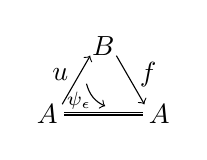
\begin{tikzpicture}[x=1.35em,y=1.35em]
  \node (Bl) at (1.5,1.8) {$B$};
  \node (Al) at (0,0) {$A$};
  \node (Ar) at (3.0,0) {$A$};
  \draw[double] (0.45,0) -- (2.55,0);
  \draw[->] (0.4,0.25) -- (1.15,1.55);
  \node at (0.35,1.05) {$u$};
  \draw[->] (1.85,1.55) -- (2.6,0.25);
  \node at (2.7,1.05) {$f$};
  \draw[->] (1.05,0.8) to[bend right=25] (1.55,0.2);
  \node at (0.85,0.35) {$\scriptstyle\psi_{\epsilon}$};
\end{tikzpicture}
\end{center}
而由引理 2.3.7，它进而定义了\trAdjunction{} $f\dashv u$ 的\trCounit{}。
\end{proof}

\begin{observation}[转置等价]\label{obs:transposing-equivalence}
为论证把诱导\trFunctor
\[
\qcor{\epsilon\cdot f(-)}\colon \mathrm{Hom}_B(B,u)\twoheadrightarrow
\mathrm{Hom}_A(f,A)
\]
称作\textbf{转置等价}（transposing equivalence）的做法，回顾如下事实：
一个 2-\trCell{} $\chi\colon b\Rightarrow ua$ 沿\trAdjunction{} $f\dashv u$
的转置，由下方左侧的粘贴图计算：
\begin{center}
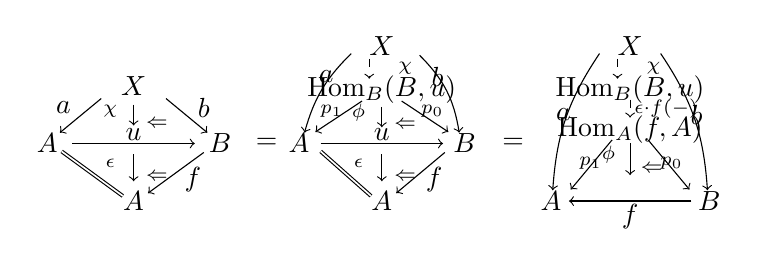
\begin{tikzpicture}[x=1.3em,y=1.3em]
  \node at (1.8,3.2) {$X$};
  \node (LA2) at (-0.6,1.6) {$A$};
  \node (LB2) at (4.2,1.6) {$B$};
  \node (LA3) at (1.8,0) {$A$};
  \draw[->] (0.9,2.85) -- (-0.25,1.9);
  \node at (-0.15,2.6) {$a$};
  \draw[->] (2.7,2.85) -- (3.85,1.9);
  \node at (3.75,2.6) {$b$};
  \draw[->] (1.8,2.68) -- (1.8,2.1);
  \node at (1.15,2.5) {$\scriptstyle\chi$};
  \node at (2.45,2.15) {$\scriptstyle\Leftarrow$};
  \draw[->] (0.1,1.6) -- (3.5,1.6);
  \node at (1.8,1.85) {$u$};
  \draw[double] (-0.2,1.38) -- (1.5,0.14);
  \draw[->] (3.75,1.35) -- (2.2,0.22);
  \node at (3.45,0.6) {$f$};
  \draw[->] (1.8,1.3) -- (1.8,0.55);
  \node at (1.15,1.05) {$\scriptstyle\epsilon$};
  \node at (2.45,0.68) {$\scriptstyle\Leftarrow$};
  \node at (5.5,1.6) {$=$};
  \node at (8.7,4.3) {$X$};
  \draw[->,dashed] (8.35,3.95) -- (8.35,3.4);
  \node at (9.35,3.68) {$\scriptstyle\qcor{\chi}$};
  \node at (8.7,3.1) {$\mathrm{Hom}_B(B,u)$};
  \draw[->] (7.85,4.1) to[bend right=15] (6.55,1.9);
  \node at (7.15,3.45) {$a$};
  \draw[->] (9.75,4.05) to[bend left=18] (10.85,1.9);
  \node at (10.25,3.45) {$b$};
  \draw[->] (8.15,2.78) -- (6.85,1.92);
  \node at (7.3,2.5) {$\scriptstyle p_1$};
  \draw[->] (9.25,2.78) -- (10.55,1.92);
  \node at (10.1,2.5) {$\scriptstyle p_0$};
  \draw[->] (8.7,2.62) -- (8.7,2.05);
  \node at (8.05,2.45) {$\scriptstyle\phi$};
  \node at (9.35,2.12) {$\scriptstyle\Leftarrow$};
  \draw[->] (7.0,1.6) -- (10.4,1.6);
  \node at (8.7,1.85) {$u$};
  \draw[double] (7.0,1.38) -- (8.4,0.14);
  \draw[->] (10.45,1.35) -- (9.1,0.22);
  \node at (10.15,0.6) {$f$};
  \draw[->] (8.7,1.3) -- (8.7,0.55);
  \node at (8.05,1.05) {$\scriptstyle\epsilon$};
  \node at (9.35,0.68) {$\scriptstyle\Leftarrow$};
  \node at (6.4,1.6) {$A$};
  \node at (11.0,1.6) {$B$};
  \node at (8.7,0) {$A$};
  \node at (12.35,1.6) {$=$};
  \node at (15.6,4.3) {$X$};
  \draw[->,dashed] (15.25,3.95) -- (15.25,3.4);
  \node at (16.25,3.68) {$\scriptstyle\qcor{\chi}$};
  \node at (15.6,3.1) {$\mathrm{Hom}_B(B,u)$};
  \draw[->] (14.75,4.1) to[bend right=15] (13.45,0.3);
  \node at (13.75,2.4) {$a$};
  \draw[->] (16.45,4.1) to[bend left=15] (17.75,0.3);
  \node at (17.45,2.4) {$b$};
  \draw[->,dashed] (15.6,2.82) -- (15.6,2.32);
  \node at (16.6,2.58) {$\scriptstyle\qcor{\epsilon\cdot f(-)}$};
  \node at (15.6,2.0) {$\mathrm{Hom}_A(f,A)$};
  \draw[->] (15.1,1.7) -- (13.95,0.32);
  \node at (14.5,1.05) {$\scriptstyle p_1$};
  \draw[->] (16.1,1.7) -- (17.25,0.32);
  \node at (16.75,1.05) {$\scriptstyle p_0$};
  \draw[->] (15.6,1.62) -- (15.6,0.72);
  \node at (15.0,1.28) {$\scriptstyle\phi$};
  \node at (16.2,0.9) {$\scriptstyle\Leftarrow$};
  \node at (13.4,0) {$A$};
  \node at (17.8,0) {$B$};
  \draw[->] (17.3,0) -- (13.9,0);
  \node at (15.6,-0.42) {$f$};
\end{tikzpicture}
\end{center}
由 $u$ 之上的右\trCommaCone{}的弱\trUniversalProperty，2-\trCell{} $\chi$
由诱导\trFunctor{} $\qcor{\chi}\colon X\to\mathrm{Hom}_B(B,u)$ 表示；
$\qcor{\chi}$ 再与转置等价复合，便定义了\trFunctor{}
$\qcor{\epsilon\cdot f(\chi)}\colon X\to\mathrm{Hom}_A(f,A)$——由自右至左的%
粘贴图等式，它所表示的正是 $\chi$ 的转置。这一观察也正当化了我们的记号：
我们为该\trFiberedEquivalence{}取名为 $\qcor{\epsilon\cdot f(-)}$，其名得自%
伴随转置的公式。
\end{observation}

\begin{corollary}\label{cor:adjunction-generalized-elements}
一对对立的\trFunctor{} $u\colon A\to B$ 与 $f\colon B\to A$ 构成一个%
\trAdjunction{} $f\dashv u$，当且仅当对任意一对\trGeneralizedElement{}
$a\colon X\to A$ 与 $b\colon Y\to B$，存在一个\trEquivalence{}
$\mathrm{Hom}_A(fb,a)\simeq_{X\times Y}\mathrm{Hom}_B(b,ua)$。
\end{corollary}

\begin{proof}
当 $f\dashv u$ 时，沿 $a\times b\colon X\times Y\to A\times B$ 的\trPullback{}%
定义了一个\trCosmologicalFunctor，它把\cref{prop:adjunction-as-fibered-equivalence}的%
\trEquivalence{} $\mathrm{Hom}_A(f,A)\simeq_{A\times B}\mathrm{Hom}_B(B,u)$
搬运为\trEquivalence{}
$\mathrm{Hom}_A(fb,a)\simeq_{X\times Y}\mathrm{Hom}_B(b,ua)$。反之，取%
\trGeneralizedElement{}为恒同\trFunctor{} $\mathrm{id}_A$ 与 $\mathrm{id}_B$
的特殊情形，即证得逆命题。
\end{proof}

\begin{remark}\label{rem:internal-mapping-spaces}
特别地，\cref{prop:adjunction-as-fibered-equivalence}的\trEquivalence{}经%
\trPullback{}定义了诸内部\trMappingSpace{}的一个\trEquivalence；内部%
\trMappingSpace{}由定义 3.4.9 引入。
在推论 12.2.15 中我们将看到：在一个由 $(\infty,1)$-\trCategory{}构成的%
\trInfinityCosmos{}中，一个\trNaturalTransformation{}
$\epsilon\colon fu\Rightarrow\mathrm{id}_A$ 定义某个\trAdjunction{}的%
\trCounit，当且仅当映射
$\qcor{\epsilon\cdot f(-)}\colon\mathrm{Hom}_B(B,u)\to\mathrm{Hom}_A(f,A)$
对任意一对元素 $a\colon\qcOne\to A$ 与 $b\colon\qcOne\to B$ 都定义内部%
\trMappingSpace{}的\trEquivalence{}
$\mathrm{Hom}_B(b,ua)\simeq\mathrm{Hom}_A(fb,a)$。
\end{remark}

\trCommaInfinityCategory{}也为表达\trUnit{}与\trCounit{}变换的%
\trUniversalProperty{}提供了一种载体。

\begin{proposition}[单位与余单位的泛性质]\label{prop:universal-property-units-counits}
考虑\trAdjunction
\begin{center}
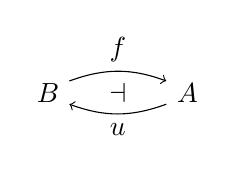
\begin{tikzpicture}[x=1.4em,y=1.4em]
  \node (B1) at (0,0) {$B$};
  \node (A1) at (3.6,0) {$A$};
  \draw[->] (0.55,0.3) to[bend left=20] node[above]{$f$} (3.05,0.3);
  \node at (1.8,0) {$\dashv$};
  \draw[->] (3.05,-0.3) to[bend left=20] node[below]{$u$} (0.55,-0.3);
\end{tikzpicture}
\end{center}
配有\trUnit{} $\eta\colon\mathrm{id}_B\Rightarrow uf$ 与\trCounit{}
$\epsilon\colon fu\Rightarrow\mathrm{id}_A$。则对每个元素
$a\colon\qcOne\to A$，分量 $\epsilon_a$ 定义了 $\mathrm{Hom}_A(f,a)$ 的一个%
\trTerminal{}元素，而对每个元素 $b\colon\qcOne\to B$，分量 $\eta_b$ 定义了
$\mathrm{Hom}_B(b,u)$ 的一个\trInitial{}元素。
\end{proposition}

\begin{proof}
\cref{prop:adjunction-as-fibered-equivalence}的\trFiberedEquivalence{}
$\mathrm{Hom}_A(f,A)\simeq_{A\times B}\mathrm{Hom}_B(B,u)$
依\cref{cor:adjunction-generalized-elements}经\trPullback{}定义了下列诸%
\trEquivalence：
\[
\mathrm{Hom}_A(f,a)\simeq_{B}\mathrm{Hom}_B(B,ua)
\qquad\text{与}\qquad
\mathrm{Hom}_A(fb,A)\simeq_{A}\mathrm{Hom}_B(b,u)
\]
由推论 3.5.10，$\mathrm{id}_{ua}$ 在 $\mathrm{Hom}_B(B,ua)$ 中诱导出一个%
\trTerminal{}元素，而由引理 2.2.7，其沿\trEquivalence{}
$\mathrm{Hom}_B(B,ua)\simeq\mathrm{Hom}_A(f,a)$ 的像仍是\trTerminal{}元素。
由\cref{obs:transposing-equivalence}，该元素表示那个转置后的 2-\trCell：即%
\trCounit{} $\epsilon$ 在元素 $a$ 处的分量。
\end{proof}

\cref{prop:universal-property-units-counits}所捕捉的\trUnit{}与\trCounit{}%
分量之\trUniversalProperty{}给出了伴随函子定理背后的主要思想。
在一个由 $(\infty,1)$-\trCategory{}构成的\trInfinityCosmos{}中，一个%
\trFunctor{} $f\colon B\to A$ 容许一个\trRightAdjoint，恰好当对每个元素
$a\colon\qcOne\to A$，\trInfinityCategory{} $\mathrm{Hom}_A(f,a)$ 容许一个%
\trTerminal{}元素（见推论 12.2.7）。
\footnote{回顾例 2.3.11：一个\trTerminal{}元素是恒同\trFunctor{}的一个%
\trColimit。Freyd 的一般伴随函子定理与特殊伴随函子定理中所部署的技术性条件，
正是为了把这个大\trColimit{}约减为小\trColimit{}并保证其存在性（这些结果的一个%
1-范畴式表述见 \cite[\S 4.6]{bib104}）。类似的定理已由 Nguyen、Raptis 与
Schrade 在 $(\infty,1)$-范畴语境中证明 \cite{bib88}。}
该\trTerminal{}元素在定义域投影函子
$p_0\colon\mathrm{Hom}_A(f,a)\twoheadrightarrow B$ 之下的像定义了元素
$ua\colon\qcOne\to B$，而\trCommaCone{}则定义了\trCounit{}在 $a$ 处的分量。
\trCounit{}分量的\trUniversalProperty{}随后被用于把元素上的这一映射扩充为
一个\trFunctor{} $u\colon A\to B$。

一个在一般\trInfinityCosmos{}中亦真的类似结果可以这样得到：把量词「对每个%
元素 $a\colon\qcOne\to A$」换成「对每个\trGeneralizedElement{}
$a\colon X\to A$」，此时「\trTerminal{}元素」的含义应当增强为「$X$ 之上的%
\trTerminal{}元素」（见定义 3.6.8）。
由于每个\trGeneralizedElement{}都经由那个泛\trGeneralizedElement{}——即 $A$
处的恒同\trFunctor{}——分解，故只需证明：

\begin{proposition}\label{prop:adjoint-criterion-terminal-element}
一个\trFunctor{} $f\colon B\to A$ 容许一个\trRightAdjoint，当且仅当
$\mathrm{Hom}_A(f,A)$ 容许一个 $A$ 之上的\trTerminal{}元素。对偶地，
$f\colon B\to A$ 容许一个\trLeftAdjoint，当且仅当 $\mathrm{Hom}_A(A,f)$
容许一个 $A$ 之上的\trInitial{}元素。
\end{proposition}

\begin{proof}
由\cref{prop:adjunction-as-fibered-equivalence}，\trFunctor{}
$f\colon B\to A$ 容许一个\trRightAdjoint，当且仅当\trCommaInfinityCategory{}
$\mathrm{Hom}_A(f,A)$ 是右\trRepresentable；而据推论 3.6.10，此情形恰在
$\mathrm{Hom}_A(f,A)$ 容许一个 $A$ 之上的\trTerminal{}元素时成立。
\end{proof}

3.5–3.6 节的同一组成果均可特化为编码\trLimit{}与\trColimit{}之%
\trUniversalProperty{}的定理。在探究这些之前，我们先来构造一个\trDiagram{}%
之上或之下的\trInfinityCategoryOfCones{}。

\subsection*{练习}

\begin{exercise}[4.3.13]\label{ex:specialize-point-adjunctions}
将\cref{prop:adjunction-as-fibered-equivalence}特化到伴随
\begin{center}
\begin{tikzpicture}[x=1.4em,y=1.4em]
  \node (P1) at (0,0) {$\qcOne$};
  \node (QA1) at (3.4,0) {$A$};
  \draw[->] (0.5,0.3) to[bend left=20] node[above]{$i$} (2.9,0.3);
  \node at (1.7,0) {$\dashv$};
  \draw[->] (2.9,-0.3) to[bend left=20] node[below]{$!$} (0.5,-0.3);
  \node at (5.2,0) {与};
  \node (P2) at (7.0,0) {$\qcOne$};
  \node (QA2) at (10.4,0) {$A$};
  \draw[->] (9.9,0.3) to[bend right=20] node[above]{$!$} (7.5,0.3);
  \node at (8.7,0) {$\dashv$};
  \draw[->] (7.5,-0.3) to[bend right=20] node[below]{$t$} (9.9,-0.3);
\end{tikzpicture}
\end{center}
的情形，以发现\trInitial{}元素与\trTerminal{}元素的另一种刻画。
\end{exercise}

\begin{exercise}\label{ex:naturality-of-transposing-equivalence}
对于任意一对平行的、完全给定的\trAdjunction
\begin{center}
\begin{tikzpicture}[x=1.4em,y=1.4em]
  \node (B1) at (0,0) {$B$};
  \node (A1) at (3.6,0) {$A$};
  \draw[->] (0.55,0.3) to[bend left=20] node[above]{$f$} (3.05,0.3);
  \node at (1.8,0) {$\dashv$};
  \draw[->] (3.05,-0.3) to[bend left=20] node[below]{$u$} (0.55,-0.3);
  \node at (5.3,0) {与};
  \node (B2) at (7.0,0) {$B$};
  \node (A2) at (10.6,0) {$A$};
  \draw[->] (7.55,0.3) to[bend left=20] node[above]{$f'$} (10.05,0.3);
  \node at (8.8,0) {$\dashv$};
  \draw[->] (10.05,-0.3) to[bend left=20] node[below]{$u'$} (7.55,-0.3);
\end{tikzpicture}
\end{center}
前者配有\trUnit{} $\eta\colon\mathrm{id}_B\Rightarrow uf$ 与\trCounit{}
$\epsilon\colon fu\Rightarrow\mathrm{id}_A$，后者配有\trUnit{}
$\eta'\colon\mathrm{id}_B\Rightarrow u'f'$ 与\trCounit{}
$\epsilon'\colon f'u'\Rightarrow\mathrm{id}_A$；则在\trNaturalTransformation{}
$\alpha\colon f'\Rightarrow f$ 与 $\beta\colon u\Rightarrow u'$ 之间存在一个%
双射，此即\emph{\trMate}（mates correspondence）的一个特例（见定义 B.3.3）。
请论证：\cref{prop:adjunction-as-fibered-equivalence}的转置等价对于「以
2-\trCell{} $\alpha\colon f'\Rightarrow f$ 作预复合」以及「以其\trMate
$\beta\colon u\Rightarrow u'$ 作后复合」（见推论 3.5.11）都是自然的，
为此请证明：在下列诸\trFunctor{}之间存在 $A\times B$ 之上的一个纤维化自然%
同构：
\begin{center}
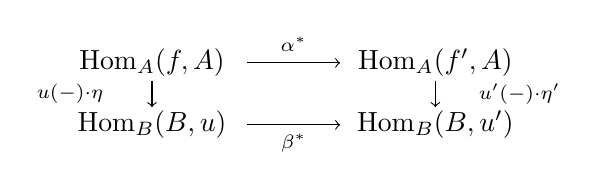
\begin{tikzpicture}[x=1.6em,y=1.6em]
  \node (TL) at (0,1.4) {$\mathrm{Hom}_A(f,A)$};
  \node (TR) at (6.4,1.4) {$\mathrm{Hom}_A(f',A)$};
  \node (BL) at (0,0) {$\mathrm{Hom}_B(B,u)$};
  \node (BR) at (6.4,0) {$\mathrm{Hom}_B(B,u')$};
  \draw[->] (2.15,1.4) -- (4.25,1.4);
  \node at (3.2,1.82) {$\scriptstyle\qcor{\alpha^{*}}$};
  \draw[->] (0,1.0) -- (0,0.4);
  \node at (-1.85,0.7) {$\scriptstyle\qcor{u(-)\cdot\eta}$};
  \draw[->] (6.4,1.0) -- (6.4,0.4);
  \node at (8.3,0.7) {$\scriptstyle\qcor{u'(-)\cdot\eta'}$};
  \draw[->] (2.15,0) -- (4.25,0);
  \node at (3.2,-0.42) {$\scriptstyle\qcor{\beta^{*}}$};
\end{tikzpicture}
\end{center}
\end{exercise}
   %
\providecommand{\qcOne}{\mathbf{1}}   %
\providecommand{\qcTwo}{\mathbf{2}}   %
\providecommand{\sSet}{s\mathcal{S}et}%

\section{\trInfinityCategoryOfCones}\label{sec:infinity-categories-of-cones}

\trCommaInfinityCategory{}构造可用于定义给定\trDiagram{}之上或之下的%
\trInfinityCategoryOfCones。由于这些∞-\trCategory{}在\trLimit{}与%
\trColimit{}之\trUniversalProperty{}的刻画中居于核心地位，我们将为这一
构造呈现几个彼此\trEquivalence{}的模型。

带有峰顶 $a\colon\qcOne\to A$ 的、\trDiagram{} $d\colon\qcOne\to A^{J}$
之上的一个\textbf{\trCone}（cone），是一个\trNaturalTransformation{}
$\lambda\Delta a\Rightarrow d$，其中 $\Delta\colon A\to A^{J}$ 是定义 2.3.1
的\trConstantFunctor。这促成了如下定义。

\begin{definition}[\trInfinityCategoryOfCones]\label{def:infinity-category-of-cones}
设 $d\colon\qcOne\to A^{J}$ 为\trInfinityCategory{} $A$ 中形状为 $J$ 的一个%
\trDiagram。$d$ \textbf{之上的\trInfinityCategoryOfCones}（∞-category of cones over $d$）%
是由\trConstantFunctor{} $\Delta$ 到 $d$ 的\trCommaInfinityCategory{}%
$\mathrm{Hom}_{A^{J}}(\Delta,d)$，而 $d$ \textbf{之下的\trInfinityCategoryOfCones}%
（∞-category of cones under $d$）则是\trCommaInfinityCategory{}%
$\mathrm{Hom}_{A^{J}}(d,\Delta)$。
\end{definition}

\begin{center}
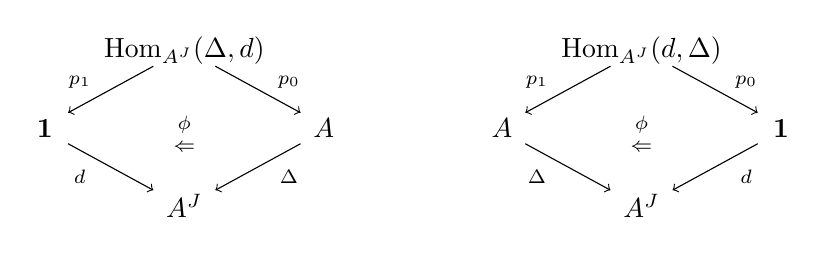
\begin{tikzpicture}[x=1.4em,y=1.4em]
  \node (h) at (0,0) {$\mathrm{Hom}_{A^{J}}(\Delta,d)$};
  \node (one) at (-3.6,-2.0) {$\qcOne$};
  \node (a) at (3.6,-2.0) {$A$};
  \node (aj) at (0,-4.0) {$A^{J}$};
  \draw[->] (-0.8,-0.4) -- (-3.0,-1.6);
  \node at (-2.7,-0.8) {$\scriptstyle p_{1}$};
  \draw[->] (0.8,-0.4) -- (3.0,-1.6);
  \node at (2.7,-0.8) {$\scriptstyle p_{0}$};
  \draw[->] (-3.0,-2.4) -- (-0.8,-3.6);
  \node at (-2.7,-3.25) {$\scriptstyle d$};
  \draw[->] (3.0,-2.4) -- (0.8,-3.6);
  \node at (2.7,-3.25) {$\scriptstyle\Delta$};
  \node at (0,-1.9) {$\scriptstyle\phi$};
  \node at (0,-2.5) {$\scriptstyle\Leftarrow$};
  \begin{scope}[shift={(11.8,0)}]
  \node (h2) at (0,0) {$\mathrm{Hom}_{A^{J}}(d,\Delta)$};
  \node (a2) at (-3.6,-2.0) {$A$};
  \node (one2) at (3.6,-2.0) {$\qcOne$};
  \node (aj2) at (0,-4.0) {$A^{J}$};
  \draw[->] (-0.8,-0.4) -- (-3.0,-1.6);
  \node at (-2.7,-0.8) {$\scriptstyle p_{1}$};
  \draw[->] (0.8,-0.4) -- (3.0,-1.6);
  \node at (2.7,-0.8) {$\scriptstyle p_{0}$};
  \draw[->] (-3.0,-2.4) -- (-0.8,-3.6);
  \node at (-2.7,-3.25) {$\scriptstyle\Delta$};
  \draw[->] (3.0,-2.4) -- (0.8,-3.6);
  \node at (2.7,-3.25) {$\scriptstyle d$};
  \node at (0,-1.9) {$\scriptstyle\phi$};
  \node at (0,-2.5) {$\scriptstyle\Leftarrow$};
  \end{scope}
\end{tikzpicture}
\end{center}

将诸\trCospan{}中「\trDiagram{}」那一支替换掉，\cref{def:infinity-category-of-cones}%
便可修改成容许 $d\colon D\to A^{J}$ 为一族\trDiagram{}的形式。在泛情形
（即 $d$ 为恒同\trFunctor{} $\mathrm{id}_{A^{J}}\colon A^{J}\to A^{J}$ 时）下，%
这就定义了形状 $J$ 的任意\trDiagram{}之上或之下的\trInfinityCategoryOfCones{}%
$\mathrm{Hom}_{A^{J}}(\Delta,A^{J})$。

在索引形状 $J$ 为一个\trSimplicialSet（而非\trCartesianClosed{}\trInfinityCosmos{}%
中的一个\trInfinityCategory）的情形，\trDiagram{}之上或之下的%
\trInfinityCategoryOfCones{}还有另一个模型：它可以由最初由 Ehlers 与 Porter
\cite{bib40} 发展出的单纯\trJoin（join）构造建造出来。
诸模型之间的\trEquivalence{}，是\trJoin{}运算与 Joyal \cite[\S9]{bib63} 引入的
所谓「\trFatJoin」（fat join）之间的\trEquivalence{}的一个推论。
正如\cref{lem:fat-join-cones}所揭示的，\trFatJoin{}构造的一个特殊实例给出%
\cref{def:infinity-category-of-cones}中出现的那些\trCone{}的形状。我们
现在引入这些概念。

\begin{definition}[\trFatJoin]\label{def:fat-join}
单纯集 $I$ 与 $J$ 的\textbf{\trFatJoin}是由如下\trPushout{}构造出的\trSimplicialSet：
\begin{center}
\begin{tikzpicture}[x=1.5em,y=1.5em]
  \node (tl) at (0,1.5) {$(I\times J)\sqcup(I\times J)$};
  \node (tr) at (7.2,1.5) {$I\sqcup J$};
  \node (bl) at (0,-1.5) {$I\times\qcTwo\times J$};
  \node (br) at (7.2,-1.5) {$I\diamond J$};
  \draw[->] (3.3,1.5) -- node[above]{$\scriptstyle\pi_{J}\sqcup\pi_{J}$} (5.5,1.5);
  \draw[right hook->] (0,0.9) -- (0,-0.9);
  \node at (2.0,0) {$\scriptstyle\ulcorner$};
  \draw[->] (2.6,-1.5) -- (5.5,-1.5);
\end{tikzpicture}
\end{center}
由此可得
\begin{equation*}
(I\diamond J)_{n}:=I_{n}\sqcup\Bigl(\coprod_{[n]\to[1]}I_{n}\times J_{n}\Bigr)\sqcup J_{n}.
\end{equation*}
注意存在自然映射 $I\diamond J\twoheadrightarrow\qcTwo$，由投影
$\pi\colon I\times\qcTwo\times J\twoheadrightarrow\qcTwo$ 诱导，使得 $I$ 是
$0$ 之上的纤维、而 $J$ 是 $1$ 之上的纤维：
\begin{center}
\begin{tikzpicture}[x=1.5em,y=1.5em]
  \node (tl) at (0,1.5) {$I\sqcup J$};
  \node (tr) at (4.6,1.5) {$I\diamond J$};
  \node (bl) at (0,-1.5) {$\qcOne+\qcOne$};
  \node (br) at (4.6,-1.5) {$\qcTwo$};
  \draw[right hook->] (1.1,1.5) -- (3.5,1.5);
  \draw[->] (0,0.9) -- (0,-0.9);
  \node at (1.6,0) {$\scriptstyle\lrcorner$};
  \draw[->] (1.3,-1.5) -- node[below]{$\scriptstyle(0,1)$} (3.3,-1.5);
\end{tikzpicture}
\end{center}
\end{definition}

任意形状为 $J$ 的\trDiagram{}之上或之下的\trInfinityCategoryOfCones{}%
可以重新描述如下。

\begin{lemma}\label{lem:fat-join-cones}
对\trInfinityCosmos{} $\mathcal{K}$ 中的任何\trSimplicialSet{} $J$ 与任何%
\trInfinityCategory{} $A$，我们有自然同构
\begin{equation*}
\mathrm{Hom}_{A^{J}}(\Delta,A^{J})\cong A^{\qcOne\diamond J}
\qquad\text{及}\qquad
\mathrm{Hom}_{A^{J}}(A^{J},\Delta)\cong A^{J\diamond\qcOne}.
\end{equation*}
\end{lemma}

\begin{proof}
单纯\trCotensor{} $A^{(-)}\colon\sSet^{\mathrm{op}}\to\mathcal{K}$ 把%
\cref{def:fat-join}的\trPushout{}送到把 $\Delta\colon A\to A^{J}$ 表示为一个%
\trCommaInfinityCategory{}的左表示与右表示所定义的那些拉回方块：
\begin{center}
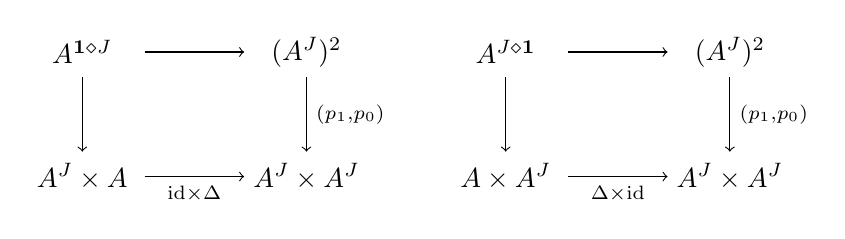
\begin{tikzpicture}[x=1.5em,y=1.5em]
  \node (tl) at (0,1.5) {$A^{\qcOne\diamond J}$};
  \node (tr) at (5.4,1.5) {$(A^{J})^{2}$};
  \node (bl) at (0,-1.5) {$A^{J}\times A$};
  \node (br) at (5.4,-1.5) {$A^{J}\times A^{J}$};
  \draw[->] (1.5,1.5) -- (3.9,1.5);
  \draw[->] (0,0.9) -- (0,-0.9);
  \node at (1.5,0) {$\scriptstyle\lrcorner$};
  \draw[->] (5.4,0.9) -- node[right]{$\scriptstyle(p_{1},p_{0})$} (5.4,-0.9);
  \draw[->] (1.5,-1.5) -- node[below]{$\scriptstyle\mathrm{id}\times\Delta$} (3.9,-1.5);
  \begin{scope}[shift={(10.2,0)}]
  \node (tl2) at (0,1.5) {$A^{J\diamond\qcOne}$};
  \node (tr2) at (5.4,1.5) {$(A^{J})^{2}$};
  \node (bl2) at (0,-1.5) {$A\times A^{J}$};
  \node (br2) at (5.4,-1.5) {$A^{J}\times A^{J}$};
  \draw[->] (1.5,1.5) -- (3.9,1.5);
  \draw[->] (0,0.9) -- (0,-0.9);
  \node at (1.5,0) {$\scriptstyle\lrcorner$};
  \draw[->] (5.4,0.9) -- node[right]{$\scriptstyle(p_{1},p_{0})$} (5.4,-0.9);
  \draw[->] (1.5,-1.5) -- node[below]{$\scriptstyle\Delta\times\mathrm{id}$} (3.9,-1.5);
  \end{scope}
\end{tikzpicture}
\end{center}
\end{proof}

\begin{definition}[\trJoin，D.2.6]\label{def:join}
单纯集 $I$ 与 $J$ 的\textbf{\trJoin}是单纯集 $I\star J$
\begin{center}
\begin{tikzpicture}[x=1.5em,y=1.5em]
  \node (tl) at (0,1.5) {$I\sqcup J$};
  \node (tr) at (4.6,1.5) {$I\star J$};
  \node (bl) at (0,-1.5) {$\qcOne+\qcOne$};
  \node (br) at (4.6,-1.5) {$\qcTwo$};
  \draw[right hook->] (1.1,1.5) -- (3.5,1.5);
  \draw[->] (0,0.9) -- (0,-0.9);
  \node at (1.6,0) {$\scriptstyle\lrcorner$};
  \draw[->] (1.3,-1.5) -- node[below]{$\scriptstyle(0,1)$} (3.3,-1.5);
\end{tikzpicture}
\qquad
其中 $\displaystyle(I\star J)_{n}:=I_{n}\sqcup\Bigl(\coprod_{0\leq k<n}I_{n-k-1}\times J_{k}\Bigr)\sqcup J_{n}$
\end{center}
并且这些 $n$-单纯形的诸顶点带有定向，使得存在典范映射
$I\star J\to\qcTwo$，其中 $I$ 是 $0$ 之上的纤维、而 $J$ 是 $1$ 之上的纤维
（更多细节见定义 D.2.2 与 D.2.6，或原始文献 \cite{bib40} 与
\cite[\S3]{bib61}）。
\end{definition}

\trJoin{}函子 $-\star J\colon\sSet\to\sSet$ 保持连通余极限，但不保持\trInitial{}对象
与其他\trCoproduct；不过，把余定义域换成 $J$ 之下的切片范畴便可达成余连续性：
函子 $-\star J\colon\sSet\to{}^{J/}\!\sSet$ 保持一切余极限（见引理 D.2.7）。
在这一语境化之下，\trJoin{}容许一个\trRightAdjoint，它由 Joyal 的\textbf{切片}%
（slice）构造定义：后者把\trSimplicialMap{} $f\colon J\to X$ 送到传统上记作 $X_{/f}$
的单纯集。

\begin{proposition}[\trJoin$\dashv$切片伴随]\label{prop:join-slice-adjunction}
诸\trJoin{}函子容许由如下自然双射定义的\trRightAdjoint：
\begin{center}
\mbox{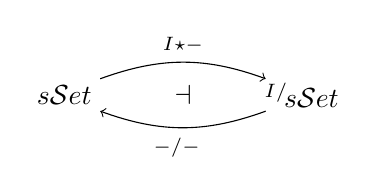
\begin{tikzpicture}[x=1.3em,y=1.3em]
  \node (s) at (0,0) {$\sSet$};
  \node (j) at (6.6,0) {${}^{I/}\!\sSet$};
  \draw[->] (1.0,0.45) to[bend left=20] node[above]{$\scriptstyle I\star-$} (5.6,0.45);
  \node at (3.3,0) {$\dashv$};
  \draw[->] (5.6,-0.45) to[bend left=20] node[below]{$\scriptstyle-/-\;\;{}$} (1.0,-0.45);
\end{tikzpicture}}
\qquad
$\left\{\,\Delta[n]\to{}^{h/}\!\!X\,\right\}:=
\left\{\vcenter{\hbox{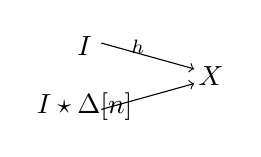
\begin{tikzpicture}[x=1.2em,y=1.2em]
  \node (i) at (0,0.9) {$I$};
  \node (m) at (0,-0.9) {$I\star\Delta[n]$};
  \node (x) at (3.8,0) {$X$};
  \draw[->] (0.5,1.0) -- (3.3,0.22);
  \node at (1.6,0.88) {$\scriptstyle h$};
  \draw[->] (0.5,-1.0) -- (3.3,-0.22);
\end{tikzpicture}}}\right\}$
\end{center}
\begin{center}
\mbox{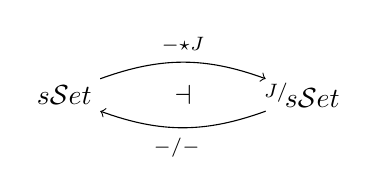
\begin{tikzpicture}[x=1.3em,y=1.3em]
  \node (s) at (0,0) {$\sSet$};
  \node (j) at (6.6,0) {${}^{J/}\!\sSet$};
  \draw[->] (1.0,0.45) to[bend left=20] node[above]{$\scriptstyle-\star J$} (5.6,0.45);
  \node at (3.3,0) {$\dashv$};
  \draw[->] (5.6,-0.45) to[bend left=20] node[below]{$\scriptstyle-/-\;\;{}$} (1.0,-0.45);
\end{tikzpicture}}
\qquad
$\left\{\,\Delta[n]\to X_{/k}\,\right\}:=
\left\{\vcenter{\hbox{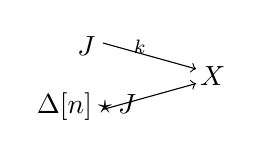
\begin{tikzpicture}[x=1.2em,y=1.2em]
  \node (i) at (0,0.9) {$J$};
  \node (m) at (0,-0.9) {$\Delta[n]\star J$};
  \node (x) at (3.8,0) {$X$};
  \draw[->] (0.5,1.0) -- (3.3,0.22);
  \node at (1.6,0.88) {$\scriptstyle k$};
  \draw[->] (0.5,-1.0) -- (3.3,-0.22);
\end{tikzpicture}}}\right\}$
\end{center}
\end{proposition}

\begin{proof}
单纯集 $X_{/k}$ 定义为其 $n$-单纯形对应于 $J$ 之下的那些映射
$\Delta[n]\star J\to X$，其上的右作用由单纯算子 $[m]\to[n]$ 经
$\Delta[m]\to\Delta[n]$ 的\trPreComposition{}给出。由于\trJoin{}函子
$-\star J\colon\sSet\to{}^{J/}\!\sSet$ 保持余极限，这就扩充成一个介于映射
$I\to X_{/k}$ 与 $J$ 之下的那些映射 $I\star J\to X$ 之间的双射，且该双射在
$I$ 与 $k\colon J\to X$ 中均自然。
\end{proof}

\begin{notation}\label{not:cone-notation}
对任何\trSimplicialSet{} $J$，我们记
\begin{equation*}
J^{\triangleleft}:=\qcOne\star J
\qquad\text{与}\qquad
J^{\triangleright}:=J\star\qcOne
\end{equation*}
并以 $\top$ 记 $J^{\triangleleft}$ 的、由终单纯集 $\qcOne$ 所贡献的那个%
\textbf{\trCone{}顶点}（cone vertex），以 $\bot$ 记 $J^{\triangleright}$ 的%
\trCone{}顶点。这些单纯集配备有典范包含
\begin{equation*}
J^{\triangleleft}\hookleftarrow J\hookrightarrow J^{\triangleright}
\end{equation*}
\end{notation}

正如其名所示，\trJoin{}与\trFatJoin{}这两个构造定义出的索引形状是彼此等价的，其意义如下。

\begin{proposition}[\trJoin{}与\trFatJoin]\label{prop:join-vs-fat-join}
对任何单纯集 $I$ 与 $J$ 以及任何\trInfinityCategory{} $A$，存在自然等价
\begin{center}
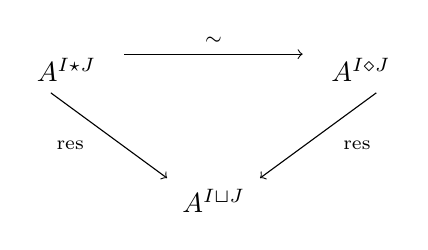
\begin{tikzpicture}[x=1.4em,y=1.4em]
  \node (l) at (0,1.6) {$A^{I\star J}$};
  \node (r) at (7.6,1.6) {$A^{I\diamond J}$};
  \node (b) at (3.8,-1.8) {$A^{I\sqcup J}$};
  \draw[->] (1.5,2.0) -- node[above]{$\scriptstyle\sim$} (6.1,2.0);
  \draw[->] (-0.4,1.0) -- (2.6,-1.2);
  \node at (0.1,-0.35) {$\scriptstyle\mathrm{res}$};
  \draw[->] (8.0,1.0) -- (5.0,-1.2);
  \node at (7.5,-0.35) {$\scriptstyle\mathrm{res}$};
\end{tikzpicture}
\end{center}
\end{proposition}

\begin{proof}
存在单纯集之间的一个典范映射
\begin{center}
\begin{tikzpicture}[x=1.5em,y=1.5em]
  \node (tl) at (0,1.6) {$(I\times J)\sqcup(I\times J)$};
  \node (tr) at (7.6,1.6) {$I\sqcup J$};
  \node (ml) at (0,-1.6) {$I\times\qcTwo\times J$};
  \node (mm) at (5.8,-1.6) {$I\diamond J$};
  \node (mr) at (10.8,-1.6) {$I\star J$};
  \node (bt) at (5.8,-4.6) {$\qcTwo$};
  \draw[->] (3.4,1.6) -- node[above]{$\scriptstyle\pi_{J}\sqcup\pi_{J}$} (5.7,1.6);
  \draw[->] (0,1.0) -- (0,-1.0);
  \node at (2.2,-0.1) {$\scriptstyle\ulcorner$};
  \draw[->] (2.4,-1.6) -- (4.5,-1.6);
  \draw[->,dashed] (7.1,-1.6) -- (9.5,-1.6);
  \draw[->] (8.1,1.3) -- (10.4,-1.1);
  \draw[->] (5.8,-2.2) -- (5.8,-4.0);
  \draw[->] (0.4,-2.2) -- (5.0,-4.4);
  \draw[->] (10.3,-2.1) -- (6.7,-4.3);
\end{tikzpicture}
\end{center}
该映射与诸纤维 $I\sqcup J$ 的包含相交换，并卧于到 $\qcTwo$ 的诸投影之上。
$I\diamond J$ 中一个不居于任一纤维之内的 $n$-单纯形，由如下三元组的数据
给定：$(\alpha\colon[n]\twoheadrightarrow[1],\ \sigma\in I_{n},\ \tau\in J_{n})$。虚线映射把这个单纯形送到代表 $I\star J$ 的一个 $n$-单纯形
的二元组 $(\sigma|_{[0,\dots,k]}\in I_{k},\ \tau|_{[k+1,\dots,n]}\in J_{n-k-1})$，其中 $k\in[n]$ 是 $\alpha^{-1}(0)$ 中的
最大顶点。附录 D 中的\cref{prop:fat-join-comparison-weak-equivalence}，
或 Lurie 的 \cite[4.2.1.2]{bib78}，证明了该映射在
$Q^{I}\times Q^{J}$ 之上诱导出诸\trQuasiCategory{}的自然等价
$Q^{I\star J}\rightsquigarrow Q^{I\diamond J}$。取 $Q$ 为\trFunctorSpace{}
$\mathrm{Fun}(X,A)$，便对一般的∞-\trCategory{}证得所宣称的等价。
\end{proof}

\begin{corollary}\label{cor:comma-squares}
对任何\trSimplicialSet{} $J$ 与\trInfinityCategory{} $A$，存在\trCommaSquare%
（comma squares）
\begin{rveq}\label{eq:comma-squares}
\mbox{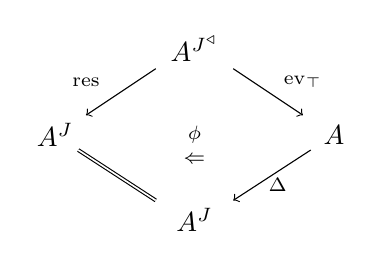
\begin{tikzpicture}[x=1.4em,y=1.4em]
  \node (t) at (0,0) {$A^{J^{\triangleleft}}$};
  \node (l) at (-3.6,-2.2) {$A^{J}$};
  \node (r) at (3.6,-2.2) {$A$};
  \node (b) at (0,-4.4) {$A^{J}$};
  \draw[->] (-1.0,-0.5) -- (-2.8,-1.7);
  \node at (-2.8,-0.85) {$\scriptstyle\mathrm{res}$};
  \draw[->] (1.0,-0.5) -- (2.8,-1.7);
  \node at (2.8,-0.85) {$\scriptstyle\mathrm{ev}_{\top}$};
  \node at (0,-2.2) {$\scriptstyle\phi$};
  \node at (0,-2.85) {$\scriptstyle\Leftarrow$};
  \draw[double] (-3.0,-2.6) -- (-1.0,-3.9);
  \draw[->] (3.0,-2.6) -- (1.0,-3.9);
  \node at (2.15,-3.5) {$\scriptstyle\Delta$};
\end{tikzpicture}}
\qquad
\mbox{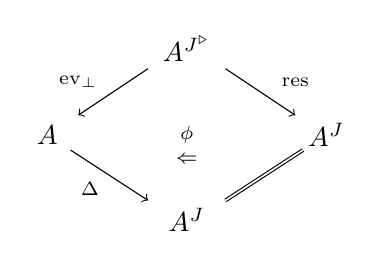
\begin{tikzpicture}[x=1.4em,y=1.4em]
  \node (t) at (0,0) {$A^{J^{\triangleright}}$};
  \node (l) at (-3.6,-2.2) {$A$};
  \node (r) at (3.6,-2.2) {$A^{J}$};
  \node (b) at (0,-4.4) {$A^{J}$};
  \draw[->] (-1.0,-0.5) -- (-2.8,-1.7);
  \node at (-2.8,-0.85) {$\scriptstyle\mathrm{ev}_{\bot}$};
  \draw[->] (1.0,-0.5) -- (2.8,-1.7);
  \node at (2.8,-0.85) {$\scriptstyle\mathrm{res}$};
  \node at (0,-2.2) {$\scriptstyle\phi$};
  \node at (0,-2.85) {$\scriptstyle\Leftarrow$};
  \draw[->] (-3.0,-2.6) -- (-1.0,-3.9);
  \node at (-2.5,-3.6) {$\scriptstyle\Delta$};
  \draw[double] (1.0,-3.9) -- (3.0,-2.6);
\end{tikzpicture}}
\end{rveq}
它们沿一族\trDiagram{} $d\colon D\to A^{J}$ 作拉回，给出 $d$ 之上或之下的%
\trInfinityCategoryOfCones{}的\trEquivalence{}模型：
\begin{center}
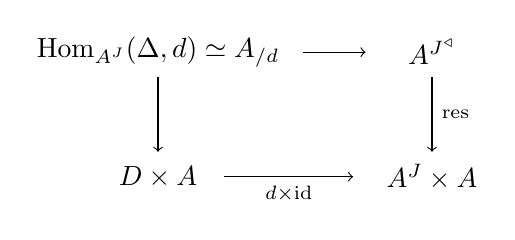
\begin{tikzpicture}[x=1.5em,y=1.5em]
  \node (h) at (0,1.5) {$\mathrm{Hom}_{A^{J}}(\Delta,d)\simeq A_{/d}$};
  \node (aj) at (6.6,1.5) {$A^{J^{\triangleleft}}$};
  \node (da) at (0,-1.5) {$D\times A$};
  \node (aa) at (6.6,-1.5) {$A^{J}\times A$};
  \draw[->] (3.5,1.5) -- (5.0,1.5);
  \draw[->] (0,0.9) -- (0,-0.9);
  \draw[->] (6.6,0.9) -- node[right]{$\scriptstyle\mathrm{res}$} (6.6,-0.9);
  \draw[->] (1.6,-1.5) -- node[below]{$\scriptstyle d\times\mathrm{id}$} (4.7,-1.5);
  \node at (2.5,-0.35) {$\scriptstyle\lrcorner$};
\end{tikzpicture}
\qquad
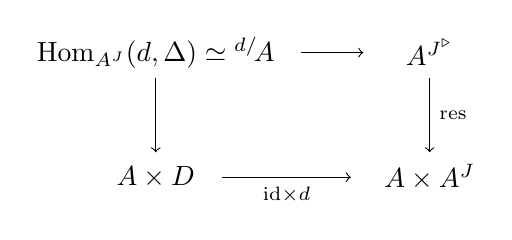
\begin{tikzpicture}[x=1.5em,y=1.5em]
  \node (h) at (0,1.5) {$\mathrm{Hom}_{A^{J}}(d,\Delta)\simeq{}^{d/}\!A$};
  \node (aj) at (6.6,1.5) {$A^{J^{\triangleright}}$};
  \node (da) at (0,-1.5) {$A\times D$};
  \node (aa) at (6.6,-1.5) {$A\times A^{J}$};
  \draw[->] (3.5,1.5) -- (5.0,1.5);
  \draw[->] (0,0.9) -- (0,-0.9);
  \draw[->] (6.6,0.9) -- node[right]{$\scriptstyle\mathrm{res}$} (6.6,-0.9);
  \draw[->] (1.6,-1.5) -- node[below]{$\scriptstyle\mathrm{id}\times d$} (4.7,-1.5);
  \node at (2.5,-0.35) {$\scriptstyle\lrcorner$};
\end{tikzpicture}
\end{center}
\end{corollary}

\begin{proof}
\cref{prop:join-vs-fat-join}构造出纤维化等价
$A^{\qcOne\diamond J}\simeq_{A^{J}\times A}A^{J^{\triangleleft}}$ 与
$A^{J\diamond\qcOne}\simeq_{A\times A^{J}}A^{J^{\triangleright}}$。由%
\cref{lem:fat-join-cones}，$A^{\qcOne\diamond J}$ 与 $A^{J\diamond\qcOne}$
是\trCommaInfinityCategory。于是，命题 3.4.11 蕴含：这些纤维化等价为
$A^{J^{\triangleleft}}$ 与 $A^{J^{\triangleright}}$ 配备上\trCommaCone，满足
命题 3.4.6 的弱\trUniversalProperty。\cref{eq:comma-squares}中的诸%
\trNaturalTransformation{}由如下诸水平复合表示
\begin{center}
\begin{tikzpicture}[x=1.4em,y=1.4em]
  \node (tl) at (0,1.6) {$J\sqcup J$};
  \node (tr) at (5.2,1.6) {$\qcOne\sqcup J$};
  \node (bl) at (0,-1.6) {$J\times\qcTwo$};
  \node (mm) at (5.2,-1.6) {$\qcOne\diamond J$};
  \node (mr) at (9.4,-1.6) {$J^{\triangleleft}$};
  \node (bt) at (5.2,-4.6) {$\qcTwo$};
  \draw[->] (1.5,1.6) -- (3.7,1.6);
  \draw[->] (0,1.0) -- (0,-1.0);
  \node at (1.7,-0.1) {$\scriptstyle\ulcorner$};
  \draw[->] (1.9,-1.6) -- (3.9,-1.6);
  \draw[->,dashed] (6.5,-1.6) -- (8.1,-1.6);
  \draw[->] (5.7,1.3) -- (9.0,-1.1);
  \draw[->] (5.2,-2.2) -- (5.2,-4.0);
  \draw[->] (0.4,-2.2) -- (4.4,-4.4);
  \draw[->] (8.9,-2.1) -- (6.1,-4.3);
\end{tikzpicture}
\qquad
\begin{tikzpicture}[x=1.4em,y=1.4em]
  \node (tl) at (0,1.6) {$J\sqcup J$};
  \node (tr) at (5.2,1.6) {$J\sqcup\qcOne$};
  \node (bl) at (0,-1.6) {$J\times\qcTwo$};
  \node (mm) at (5.2,-1.6) {$J\diamond\qcOne$};
  \node (mr) at (9.4,-1.6) {$J^{\triangleright}$};
  \node (bt) at (5.2,-4.6) {$\qcTwo$};
  \draw[->] (1.5,1.6) -- (3.7,1.6);
  \draw[->] (0,1.0) -- (0,-1.0);
  \node at (1.7,-0.1) {$\scriptstyle\ulcorner$};
  \draw[->] (1.9,-1.6) -- (3.9,-1.6);
  \draw[->,dashed] (6.5,-1.6) -- (8.1,-1.6);
  \draw[->] (5.7,1.3) -- (9.0,-1.1);
  \draw[->] (5.2,-2.2) -- (5.2,-4.0);
  \draw[->] (0.4,-2.2) -- (4.4,-4.4);
  \draw[->] (8.9,-2.1) -- (6.1,-4.3);
\end{tikzpicture}
\end{center}
将它们作\trCotensor{}射入 $A$，便产生自然变换：
\begin{center}
\begin{tikzpicture}[x=1.15em,y=1.4em]
  \node (l) at (0,0) {$A^{J^{\triangleleft}}$};
  \node (m) at (6.0,0) {$(A^{J})^{2}$};
  \node (r) at (12.0,0) {$A^{J}$};
  \draw[->] (1.9,0.35) to[bend left=18] (4.7,0.35);
  \node at (3.0,1.05) {$\scriptstyle\Delta\mathrm{ev}_{\top}$};
  \draw[->] (1.9,-0.35) to[bend right=18] (4.7,-0.35);
  \node at (3.0,-1.05) {$\scriptstyle\mathrm{res}$};
  \draw[->] (7.4,0.35) to[bend left=18] (10.5,0.35);
  \node at (8.4,1.05) {$\scriptstyle p_{0}$};
  \draw[->] (8.95,0.2) to[bend right=35] (8.95,-0.2);
  \node at (9.95,0) {$\scriptstyle\psi_{\kappa}$};
  \node at (8.4,-1.05) {$\scriptstyle p_{1}$};
  \draw[->] (7.4,-0.35) to[bend right=18] (10.5,-0.35);
  \node at (14.6,0) {与};
  \begin{scope}[shift={(17.2,0)}]
  \node (l2) at (0,0) {$A^{J^{\triangleright}}$};
  \node (m2) at (6.0,0) {$(A^{J})^{2}$};
  \node (r2) at (12.0,0) {$A^{J}$};
  \draw[->] (1.9,0.35) to[bend left=18] (4.7,0.35);
  \node at (3.0,1.05) {$\scriptstyle\mathrm{res}$};
  \draw[->] (1.9,-0.35) to[bend right=18] (4.7,-0.35);
  \node at (3.0,-1.05) {$\scriptstyle\Delta\mathrm{ev}_{\bot}$};
  \draw[->] (7.4,0.35) to[bend left=18] (10.5,0.35);
  \node at (8.4,1.05) {$\scriptstyle p_{0}$};
  \draw[->] (8.95,0.2) to[bend right=35] (8.95,-0.2);
  \node at (9.95,0) {$\scriptstyle\psi_{\kappa}$};
  \node at (8.4,-1.05) {$\scriptstyle p_{1}$};
  \draw[->] (7.4,-0.35) to[bend right=18] (10.5,-0.35);
  \end{scope}
\end{tikzpicture}
\end{center}
这些纤维化等价经拉回，即为固定的一族\trDiagram{} $d$ 之上或之下的%
\trInfinityCategoryOfCones{}给出\trEquivalence{}的模型。
\end{proof}

\begin{warning}\label{war:slice-notation}
在\cref{cor:comma-squares}的陈述与其他场合，对\trDiagram{}
$d\colon\qcOne\to A^{J}$ 之上的诸限制映射的诸\trFiber，借用 Joyal 的切片
记号颇为便利。这一用法的正当性由附录 D 中的%
\cref{prop:slices-cones-equivalence}给出：后者在\trQuasiCategory{}%
的\trInfinityCosmos{}中证明 $A_{/d}\simeq_{A}\mathrm{Hom}_{A^{J}}(\Delta,d)$
与 ${}^{d/}\!A\simeq_{A}\mathrm{Hom}_{A^{J}}(d,\Delta)$。然而请注意，在%
\trQuasiCategory{}的\trInfinityCosmos{}中，这些严格纤维并\emph{不}同构于
Joyal 的切片拟范畴（见\cref{ex:fiber-of-cone-category}），而仅仅是等价于
它们。
\end{warning}

\subsection*{练习}

\begin{exercise}\label{ex:join-vs-fat-join-section}
计算 $\Delta[n]\star\Delta[m]$ 与 $\Delta[n]\diamond\Delta[m]$，并对%
\cref{prop:join-vs-fat-join}之证明中所构造的那个映射定义一个\trSection
\begin{equation*}
\Delta[n]\star\Delta[m]\longrightarrow\Delta[n]\diamond\Delta[m]
\end{equation*}
\end{exercise}

\begin{exercise}\label{ex:fiber-of-cone-category}
在\trQuasiCategory{}的\trInfinityCosmos{}中，计算 $A^{J^{\triangleleft}}\twoheadrightarrow A^{J}$ 在 $d\colon\qcOne\to A^{J}$ 之上的\trFiber，并
证明该\trQuasiCategory{}不同构于 $A_{/d}$。
\end{exercise}

\begin{exercise}[{\cite[3.5]{bib63}}]\label{ex:join-dependent-product}
作为预层\trCategory{}的单纯集\trCategory{}是\textbf{局部\trCartesianClosed}%
（locally cartesian closed），意思是与任何映射 $f\colon U\to V$ 相关联的%
\trPullback{}函子都容许一个\trRightAdjoint{} $\Pi_{f}$，称为\textbf{依依赖积}%
（dependent product）或\textbf{前推}（pushforward）：
\begin{center}
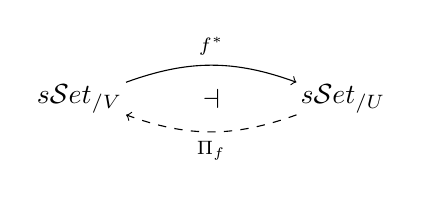
\begin{tikzpicture}[x=1.4em,y=1.4em]
  \node (l) at (0,0) {$\sSet_{/V}$};
  \node (r) at (6.8,0) {$\sSet_{/U}$};
  \draw[->] (1.2,0.42) to[bend left=20] node[above]{$\scriptstyle f^{*}$} (5.6,0.42);
  \node at (3.4,0) {$\dashv$};
  \draw[->,dashed] (5.6,-0.42) to[bend left=20] node[below]{$\scriptstyle\Pi_{f}$} (1.2,-0.42);
\end{tikzpicture}
\end{center}
证明：\trJoin{} $I\star J$ 可以定义为 $\sSet_{/\qcTwo}$ 中的一个对象，即沿
$\qcOne+\qcOne\hookrightarrow\qcTwo$ 取 $!\sqcup!\colon I\sqcup J\to\qcOne+\qcOne$ 的依依赖积。
\end{exercise}
   %
\providecommand{\qcOne}{\mathbf{1}}   %
\providecommand{\qcor}[1]{\ulcorner#1\urcorner}   %
\providecommand{\ShapeSpan}{\sqcap}    %
\providecommand{\ShapeCospan}{\sqcup}  %
\providecommand{\ShapeSquare}{\square} %

\section{\trLimit{}与\trColimit{}的\trUniversalProperty}\label{sec:universal-property-of-limits-and-colimits}

为了刻画\trLimit{}与\trColimit{}的\trUniversalProperty{}，我们回到定义 2.3.1 的
一般语境，同时考虑取值于某个\trInfinityCategory{}、且由一个\trSimplicialSet{}%
或另一个\trInfinityCategory{}索引的\trDiagram{}，此时要求环境\trInfinityCosmos{}%
\trCartesianClosed{}。正如命题 4.1.1 的情形，定理 3.5.8 立即特化到定义 2.3.8 的
框架，证得：

\begin{proposition}[余/极限表示锥]\label{prop:colimits-represent-cones}
一族\trDiagram{} $d\colon D\to A^{J}$ 容许一个\trLimit{}，当且仅当 $d$ 之上的%
\trInfinityCategoryOfCones{} $\mathrm{Hom}_{A^{J}}(\Delta,d)$ 是右\trRepresentable
\begin{equation*}
\mathrm{Hom}_{A^{J}}(\Delta,d)\simeq_{D\times A}\mathrm{Hom}_{A}(A,\ell),
\end{equation*}
此时表示函子 $\ell\colon D\to A$ 定义出\trLimit{}函子。对偶地，一族\trDiagram{}
$d\colon D\to A^{J}$ 容许一个\trColimit{}，当且仅当 $d$ 之下的%
\trInfinityCategoryOfCones{} $\mathrm{Hom}_{A^{J}}(d,\Delta)$ 是左\trRepresentable
\begin{equation*}
\mathrm{Hom}_{A^{J}}(d,\Delta)\simeq_{A\times D}\mathrm{Hom}_{A}(c,A),
\end{equation*}
此时表示函子 $c\colon D\to A$ 定义出\trColimit{}函子。
\end{proposition}

推论 3.6.10 特化后告诉我们：这样的表示可以由\trTerminal{}\trElement{}或%
\trInitial{}\trElement{}来编码；这一结果在单个\trDiagram{}（而非\trDiagram{}族）
的情形最易解读。

\begin{proposition}[\trLimit{}作为\trTerminal\trCone]\label{prop:limits-as-terminal-cones}
\trInfinityCategory{} $A$ 中形状为 $J$ 的一个\trDiagram{} $d\colon\qcOne\to A^{J}$
(i) 容许一个\trLimit{}，当且仅当 $d$ 之上的\trInfinityCategoryOfCones{}
$\mathrm{Hom}_{A^{J}}(\Delta,d)$ 容许一个\trTerminal{}\trElement{}，此时该%
\trTerminal{}\trElement{}定义一个\trLimit\trCone{}；而
(ii) 容许一个\trColimit{}，当且仅当 $d$ 之下的\trInfinityCategoryOfCones{}
$\mathrm{Hom}_{A^{J}}(d,\Delta)$ 容许一个\trInitial{}\trElement{}，此时该%
\trInitial{}\trElement{}定义\trColimit\trCone{}。
\end{proposition}

\trLimit\trCone{}与\trColimit\trCone{}在同构意义下的唯一性，可由应用引理 2.2.3
得到；亦可从绝对提升图刻画出发证明（见练习 2.3.vi）。

\begin{remark}\label{rem:family-limit-terminal-element}
推论 3.6.10 同样适用于断言：一族\trDiagram{} $d\colon D\to A^{J}$ 容许一个%
\trLimit{}，恰好当 $\mathrm{Hom}_{A^{J}}(\Delta,d)$ 容许一个 $D$ 之上的%
\trTerminal{}\trElement{}；而容许一个\trColimit{}，恰好当
$\mathrm{Hom}_{A^{J}}(d,\Delta)$ 容许一个 $D$ 之上的\trInitial{}\trElement{}。
\end{remark}

出于审美上的理由，下面两个结果我们只对由\trSimplicialSet{}索引的\trDiagram{}%
来陈述，以便使用更优雅、或许更易于解读的记号。正如\cref{ex:j-indexed-versions}
所揭示的，并没有数学上的理由要限制在这一特殊情形。%
\footnote{事实上，证明实际使用的是余定义域投影函子
$p_{1}\colon\mathrm{Hom}_{A^{J}}(\Delta,A^{J})\twoheadrightarrow A^{J}$，而非与之%
\trEquivalence{}的等价纤维化
$\mathrm{res}\colon A^{J^{\triangleleft}}\twoheadrightarrow A^{J}$，因此这一更
朴素的论证同样适用于由\trInfinityCategory{} $J$ 索引\trDiagram{}的情形——无论
其所处的\trCartesianClosed{}\trInfinityCosmos{}是否容许可用于索引形状的联接运算。}

\begin{proposition}\label{prop:absolute-right-lifting-res}
一个\trInfinityCategory{} $A$ 容许由\trSimplicialSet{} $J$ 索引的一族\trDiagram{}
$d\colon D\to A^{J}$ 的\trLimit{}，当且仅当 $d$ 沿限制函子
\begin{center}
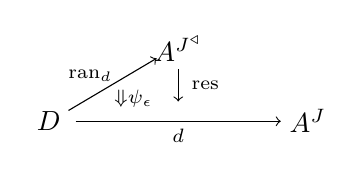
\begin{tikzpicture}[x=1.3em,y=1.3em]
  \node (Ajt) at (3.6,2.0) {$A^{J^{\triangleleft}}$};
  \node (D) at (0,0) {$D$};
  \node (Aj) at (7.2,0) {$A^{J}$};
  \draw[->] (0.55,0.3) -- (3.0,1.75);
  \node at (1.15,1.25) {$\scriptstyle\mathrm{ran}_{d}$};
  \draw[->] (3.6,1.45) -- (3.6,0.55);
  \node at (4.35,1.0) {$\scriptstyle\mathrm{res}$};
  \draw[->] (0.75,0) -- (6.45,0);
  \node at (3.6,-0.4) {$\scriptstyle d$};
  \node at (2.35,0.62) {$\scriptstyle\Downarrow\psi_{\epsilon}$};
\end{tikzpicture}
\end{center}
存在一个绝对右\trLifting{}。当这些等价条件成立时，$\epsilon$ 必为同构，且可取为
恒同。
\end{proposition}

\begin{proof}
依定义 2.3.8，一族\trDiagram{} $d$ 容许一个\trLimit{}，当且仅当它沿
$\Delta\colon A\to A^{J}$ 容许一个绝对右\trLifting{}。依命题 3.6.14，这一绝对提升
存在，当且仅当 $d$ 沿余定义域投影函子
$p_{1}\colon\mathrm{Hom}_{A^{J}}(\Delta,A^{J})\to A^{J}$ 容许一个绝对右\trLifting{}，
此时后一绝对右提升图表的自然同构是可逆的。依推论 4.2.8，限制函子
$\mathrm{res}\colon A^{J^{\triangleleft}}\twoheadrightarrow A^{J}$ \trEquivalence{}于这一余定义域
投影函子，故练习 3.5.ii 蕴含：$d$ 沿 $p_{1}$ 的绝对右提升等价于 $d$ 沿
$\mathrm{res}$ 的绝对右提升。若这一绝对提升图由一个可逆 2-胞腔充实，则命题 1.4.9
所证的等价纤维化的同构提升性质，可用来把函子
$\mathrm{ran}_{d}\colon D\to A^{J^{\triangleleft}}$ 替换为同构的函子，得到一个
严格交换的三角，且依练习 2.3.vi 它仍是绝对右提升图表。
\end{proof}

\cref{prop:absolute-right-lifting-res}特化后给出一个结构化的刻画，针对那些容许
特定形状的一切\trLimit{}或一切\trColimit{}的\trInfinityCategory{}（见定义 2.3.2）。

\begin{corollary}\label{cor:res-fibered-adjoints}
一个\trInfinityCategory{} $A$ 容许由\trSimplicialSet{} $J$ 索引的一切\trLimit{}，
当且仅当左下图的限制函子在 $A^{J}$ 之上容许一个\trFibered\trRightAdjoint{}；而 $A$
容许由\trSimplicialSet{} $J$ 索引的一切\trColimit{}，当且仅当右下图的限制函子在
$A^{J}$ 之上容许一个\trFibered\trLeftAdjoint{}。
\begin{center}
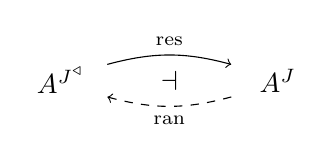
\begin{tikzpicture}[x=1.4em,y=1.4em]
  \node (l) at (0,0) {$A^{J^{\triangleleft}}$};
  \node (r) at (5.6,0) {$A^{J}$};
  \draw[->] (1.2,0.42) to[bend left=15] node[above]{$\scriptstyle\mathrm{res}$} (4.4,0.42);
  \node at (2.8,0) {$\dashv$};
  \draw[->,dashed] (4.4,-0.42) to[bend left=15] node[below]{$\scriptstyle\mathrm{ran}$} (1.2,-0.42);
\end{tikzpicture}
\qquad
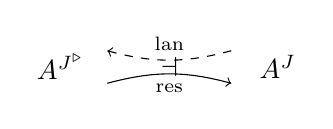
\begin{tikzpicture}[x=1.4em,y=1.4em]
  \node (l) at (0,0) {$A^{J^{\triangleright}}$};
  \node (r) at (5.6,0) {$A^{J}$};
  \draw[->,dashed] (4.4,0.42) to[bend left=15] node[above]{$\scriptstyle\mathrm{lan}$} (1.2,0.42);
  \node at (2.8,0) {$\dashv$};
  \draw[->] (1.2,-0.42) to[bend left=15] node[below]{$\scriptstyle\mathrm{res}$} (4.4,-0.42);
\end{tikzpicture}
\end{center}
\end{corollary}

\begin{proof}
依\cref{prop:absolute-right-lifting-res}与引理 2.3.7，$A$ 容许一切 $J$ 形状的%
\trLimit{}，当且仅当函子 $\mathrm{res}\colon A^{J^{\triangleleft}}\twoheadrightarrow A^{J}$ 容许
一个\trRightAdjoint\trRightInverse{}。由于限制函子是一个等价纤维化，引理 3.6.9
适用，可将该\trRightAdjoint\trRightInverse\trRectify{}为一个\trFibered\trAdjunction{}。
\end{proof}

现在，我们把已发展的一般理论应用到一些特定的索引形状上。

\begin{definition}[\trTensor{}与\trCotensor]\label{def:tensors-cotensors}
设 $K$ 为一个\trSimplicialSet{}，并设 $a\colon\qcOne\to A$ 为某个\trInfinityCategory{}
$A$ 的一个\trElement{}。$a$ 经 $K$ 的\textbf{\trTensor}（tensor）$K\otimes a$，是取值为
$a$ 的常值 $K$-索引\trDiagram{}的\trColimit{}；而 $a$ 经 $K$ 的%
\textbf{\trCotensor}（cotensor）$a^{K}$，则是同一\trDiagram{}的\trLimit{}。于是，
\trTensor{}函子与\trCotensor{}函子可由下列绝对提升图定义：
\begin{center}
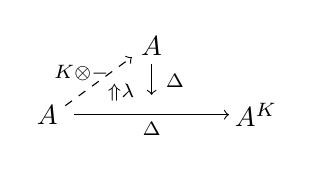
\begin{tikzpicture}[x=1.3em,y=1.3em]
  \node (At) at (2.9,1.9) {$A$};
  \node (Al) at (0,0) {$A$};
  \node (Ak) at (5.8,0) {$A^{K}$};
  \draw[->,dashed] (0.5,0.25) -- (2.35,1.6);
  \node at (0.95,1.15) {$\scriptstyle K\otimes-$};
  \draw[->] (2.9,1.4) -- (2.9,0.55);
  \node at (3.55,0.95) {$\scriptstyle\Delta$};
  \draw[->] (0.75,0) -- (5.05,0);
  \node at (2.9,-0.4) {$\scriptstyle\Delta$};
  \node at (2.05,0.62) {$\scriptstyle\Uparrow\lambda$};
\end{tikzpicture}
\qquad
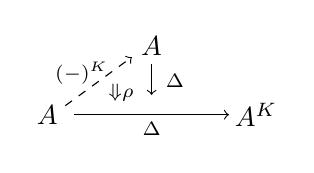
\begin{tikzpicture}[x=1.3em,y=1.3em]
  \node (At) at (2.9,1.9) {$A$};
  \node (Al) at (0,0) {$A$};
  \node (Ak) at (5.8,0) {$A^{K}$};
  \draw[->,dashed] (0.5,0.25) -- (2.35,1.6);
  \node at (0.95,1.15) {$\scriptstyle(-)^{K}$};
  \draw[->] (2.9,1.4) -- (2.9,0.55);
  \node at (3.55,0.95) {$\scriptstyle\Delta$};
  \draw[->] (0.75,0) -- (5.05,0);
  \node at (2.9,-0.4) {$\scriptstyle\Delta$};
  \node at (2.05,0.62) {$\scriptstyle\Downarrow\rho$};
\end{tikzpicture}
\end{center}
依定理 3.5.3，这些绝对提升图定义出纤维化等价
\begin{equation*}
\mathrm{Hom}_{A}(K\otimes-,A)\simeq_{A\times A}\mathrm{Hom}_{A^{K}}(\Delta,\Delta)
\simeq_{A\times A}\mathrm{Hom}_{A}(A,(-)^{K}),
\end{equation*}
二者复合，便定义出编码\trTensor{}函子与\trCotensor{}函子之间一个\trAdjunction{}的%
\trFiberedEquivalence{}：
\begin{center}
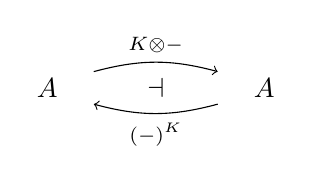
\begin{tikzpicture}[x=1.4em,y=1.4em]
  \node (l) at (0,0) {$A$};
  \node (r) at (5.6,0) {$A$};
  \draw[->] (1.2,0.42) to[bend left=15] node[above]{$\scriptstyle K\otimes-$} (4.4,0.42);
  \node at (2.8,0) {$\dashv$};
  \draw[->] (4.4,-0.42) to[bend left=15] node[below]{$\scriptstyle(-)^{K}$} (1.2,-0.42);
\end{tikzpicture}
\end{center}
依推论 4.1.3，表达\trTensor{}与\trCotensor{}之\trUniversalProperty{}的那些%
\trFiberedEquivalence{}沿元素 $a,x\colon\qcOne\to A$ 作\trPullback{}，定义出%
\trMappingSpace{}的等价：
\begin{equation*}
\begin{gathered}
\mathrm{Hom}_{A}(K\otimes a,x)\cong\mathrm{Hom}_{A^{K}}(\Delta a,\Delta x)
\cong\mathrm{Hom}_{A}(a,x)^{K}\qquad\text{与}\\
\mathrm{Hom}_{A}(x,a^{K})\cong\mathrm{Hom}_{A^{K}}(\Delta x,\Delta a)
\cong\mathrm{Hom}_{A}(x,a)^{K}.
\end{gathered}
\end{equation*}
\end{definition}

\begin{definition}[\trSpan{}与\trCospan]\label{def:span-cospan}
\trInfinityCategory{} $A$ 中的一个\textbf{\trSpan}（span），是由单纯集
$\ShapeSpan:=\Lambda^{0}[2]$ 索引的\trDiagram{}，后者由两条 $1$-单纯形沿其定义域
顶点粘合而成。对偶地，$A$ 中的一个\textbf{\trCospan}（cospan），是由单纯集
$\ShapeCospan:=\Lambda^{2}[2]$ 索引的\trDiagram{}，后者由两条 $1$-单纯形沿其余
定义域顶点粘合而成。\trInfinityCategory{} $A$ 中的余跨度与跨度，可分别由把一对
箭头沿其公共余定义域或公共定义域粘合而定义：

\begin{center}
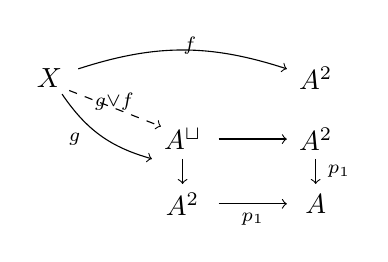
\begin{tikzpicture}[x=1.3em,y=1.3em]
  \node (X) at (0,2.6) {$X$};
  \node (Art) at (7.4,2.6) {$A^{2}$};
  \node (Acup) at (3.7,0.9) {$A^{\ShapeCospan}$};
  \node (Arm) at (7.4,0.9) {$A^{2}$};
  \node (Ab) at (3.7,-0.9) {$A^{2}$};
  \node (A) at (7.4,-0.9) {$A$};
  \draw[->] (0.8,2.85) to[bend left=18] (6.6,2.85);
  \node at (3.9,3.5) {$\scriptstyle f$};
  \draw[->,dashed] (0.55,2.25) -- (3.1,1.25);
  \node at (1.8,1.95) {$\scriptstyle g\vee f$};
  \draw[->] (0.35,2.15) to[bend right=20] (2.85,0.35);
  \node at (0.7,0.9) {$\scriptstyle g$};
  \draw[->] (4.7,0.9) -- (6.6,0.9);
  \draw[->] (3.7,0.35) -- (3.7,-0.35);
  \draw[->] (7.4,0.35) -- (7.4,-0.35);
  \node at (8.05,0.0) {$\scriptstyle p_{1}$};
  \draw[->] (4.7,-0.9) -- (6.6,-0.9);
  \node at (5.65,-1.32) {$\scriptstyle p_{1}$};
  \node at (5.1,0.35) {$\scriptstyle\lrcorner$};
\end{tikzpicture}
\qquad
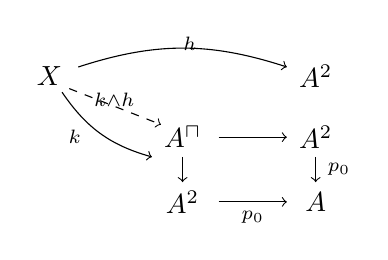
\begin{tikzpicture}[x=1.3em,y=1.3em]
  \node (X) at (0,2.6) {$X$};
  \node (Art) at (7.4,2.6) {$A^{2}$};
  \node (Acup) at (3.7,0.9) {$A^{\ShapeSpan}$};
  \node (Arm) at (7.4,0.9) {$A^{2}$};
  \node (Ab) at (3.7,-0.9) {$A^{2}$};
  \node (A) at (7.4,-0.9) {$A$};
  \draw[->] (0.8,2.85) to[bend left=18] (6.6,2.85);
  \node at (3.9,3.5) {$\scriptstyle h$};
  \draw[->,dashed] (0.55,2.25) -- (3.1,1.25);
  \node at (1.8,1.95) {$\scriptstyle k\wedge h$};
  \draw[->] (0.35,2.15) to[bend right=20] (2.85,0.35);
  \node at (0.7,0.9) {$\scriptstyle k$};
  \draw[->] (4.7,0.9) -- (6.6,0.9);
  \draw[->] (3.7,0.35) -- (3.7,-0.35);
  \draw[->] (7.4,0.35) -- (7.4,-0.35);
  \node at (8.05,0.0) {$\scriptstyle p_{0}$};
  \draw[->] (4.7,-0.9) -- (6.6,-0.9);
  \node at (5.65,-1.32) {$\scriptstyle p_{0}$};
  \node at (5.1,0.35) {$\scriptstyle\lrcorner$};
\end{tikzpicture}
\end{center}
\end{definition}

\begin{definition}[\trPushout{}与\trPullback]\label{def:pushout-pullback}
\trInfinityCategory{} $A$ 中的一个\textbf{\trPushout}（pushout），是由单纯集
$\ShapeSpan$ 索引的\trDiagram{}的\trColimit{}；而一个\textbf{\trPullback}
（pullback）则是\trInfinityCategory{} $A$ 中由单纯集 $\ShapeCospan$ 索引的%
\trDiagram{}的\trLimit{}。形状为 $\ShapeCospan$ 的\trDiagram{}之上的\trCone{}或
形状为 $\ShapeSpan$ 的\trDiagram{}之下的\trCone{}，定义出\textbf{交换方块}
（commutative squares），即形状为
\begin{equation*}
\ShapeSquare:=\ShapeSpan^{\triangleright}\cong 2\times 2\cong\ShapeCospan^{\triangleleft}
\end{equation*}
的\trDiagram{}。

\trInfinityCategory{} $A$ 中的一个\textbf{拉回方块}（pullback square），是
$A^{\ShapeSquare}$ 的一个\trElement{}，它定义出其底下的余跨度的一个绝对右\trLifting{}：
\begin{center}
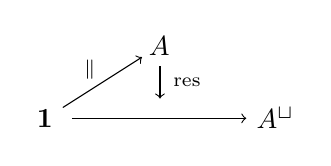
\begin{tikzpicture}[x=1.3em,y=1.3em]
  \node (Asq) at (3.2,2.0) {$A^{\ShapeSquare}$};
  \node (One) at (0,0) {$\qcOne$};
  \node (Acup) at (6.4,0) {$A^{\ShapeCospan}$};
  \draw[->] (0.5,0.3) -- (2.7,1.7);
  \node at (1.25,1.35) {$\scriptstyle\parallel$};
  \draw[->] (3.2,1.45) -- (3.2,0.55);
  \node at (3.95,1.0) {$\scriptstyle\mathrm{res}$};
  \draw[->] (0.75,0) -- (5.6,0);
\end{tikzpicture}
\qquad
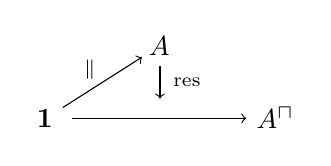
\begin{tikzpicture}[x=1.3em,y=1.3em]
  \node (Asq) at (3.2,2.0) {$A^{\ShapeSquare}$};
  \node (One) at (0,0) {$\qcOne$};
  \node (Acup) at (6.4,0) {$A^{\ShapeSpan}$};
  \draw[->] (0.5,0.3) -- (2.7,1.7);
  \node at (1.25,1.35) {$\scriptstyle\parallel$};
  \draw[->] (3.2,1.45) -- (3.2,0.55);
  \node at (3.95,1.0) {$\scriptstyle\mathrm{res}$};
  \draw[->] (0.75,0) -- (5.6,0);
\end{tikzpicture}
\end{center}
当 $A$ 容许一切\trPullback{}时，拉回方块可以刻画为 $A^{\ShapeSquare}$ 中使%
\cref{cor:res-fibered-adjoints}的\trAdjunction{} $\mathrm{res}\dashv\mathrm{ran}$
之\trUnit{}分量为同构的那些\trElement{}（见\cref{ex:family-pullback-criteria}）。
对偶地，$A$ 中的一个\textbf{推出方块}（pushout square），是 $A^{\ShapeSquare}$ 的
一个\trElement{}，它定义出其底下的跨度的一个绝对左\trLifting{}，亦即使\trAdjunction
$\mathrm{lan}\dashv\mathrm{res}$ 之\trCounit{}分量为同构的\trElement{}。由推出方块
或拉回方块构成的一族 $X\to A^{\ShapeSquare}$ 之概念可类似定义。
\end{definition}

拉回方块可用绝对提升图来刻画，这对建立它们的基本演算颇为有用。为此，我们使用
下述引理。

\begin{lemma}\label{lem:postcomposition}
考虑一族箭头 $f\colon X\to A^{2}$，它表示一个自然变换
\begin{center}
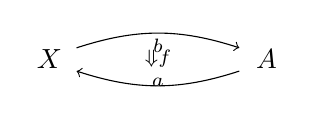
\begin{tikzpicture}[x=1.4em,y=1.2em]
  \node (X) at (0,0) {$X$};
  \node (A) at (5.6,0) {$A$};
  \draw[->] (0.7,0.35) to[bend left=18] (4.9,0.35);
  \node at (2.8,0.42) {$\scriptstyle b$};
  \node at (2.8,0.02) {$\scriptstyle\Downarrow f$};
  \draw[->] (4.9,-0.35) to[bend left=18] (0.7,-0.35);
  \node at (2.8,-0.68) {$\scriptstyle a$};
\end{tikzpicture}
\end{center}
那么存在一个跨度
\begin{center}
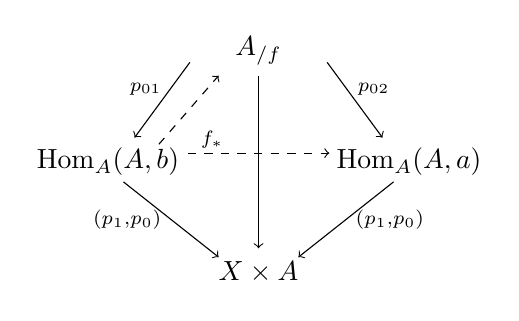
\begin{tikzpicture}[x=1.6em,y=1.6em]
  \node (Af) at (3.4,2.5) {$A_{/f}$};
  \node (Hb) at (0,0) {$\mathrm{Hom}_{A}(A,b)$};
  \node (Ha) at (6.8,0) {$\mathrm{Hom}_{A}(A,a)$};
  \node (XA) at (3.4,-2.5) {$X\times A$};
  \draw[->] (1.85,2.25) -- (0.6,0.55);
  \node at (0.85,1.65) {$\scriptstyle p_{01}$};
  \draw[->] (4.95,2.25) -- (6.2,0.55);
  \node at (6.0,1.65) {$\scriptstyle p_{02}$};
  \draw[->,dashed] (1.15,0.4) -- (2.5,1.95);%
  \draw[->,dashed] (1.8,0.2) -- (5.0,0.2);
  \node at (2.35,0.5) {$\scriptstyle f_{*}$};
  \draw[->] (3.4,1.95) -- (3.4,-1.95);
  \draw[->] (0.35,-0.45) -- node[left]{$\scriptstyle(p_{1},p_{0})$} (2.5,-2.15);
  \draw[->] (6.45,-0.45) -- node[right]{$\scriptstyle(p_{1},p_{0})$} (4.3,-2.15);
\end{tikzpicture}
\end{center}
使得任何到平凡纤维化 $p_{01}$ 的截面与 $p_{02}$ 复合，都定义出一个表示以 $f$ 作%
\trPostComposition{}的函子 $f_{*}$；而且 $f_{*}$ 的\trFiberedIsomorphism{}类中的
每个函子都按此方式产生。%
\footnote{推论 3.5.11 在\trHomotopyTwoCategory{}中的自然变换
$\alpha\colon b\Rightarrow a$ 与函子
$\qcor{\alpha_{*}}\colon\mathrm{Hom}_{A}(A,b)\to\mathrm{Hom}_{A}(A,a)$ 之间，在%
\trFiberedIsomorphism{}的意义下定义了一个双射。此处我们稍稍改变记号，因为我们是
从一族箭头 $f\colon X\to A^{2}$ 出发，而非从该族所表示的那个自然变换出发。}
此外，$f$ 表示一个自然同构 $f\colon b\cong a$，\footnote{原书印作
『$f:a\cong b$』，与其所示自然变换 $f\colon b\Rightarrow a$ 方向相悖，疑为笔误，
此处径改。——译者注}当且仅当等价纤维化 $p_{02}$ 是一个平凡纤维化。
\end{lemma}

\begin{proof}
通过构造每一列的拉回，下方的余跨度之跨度便定义出陈述中那个跨度的对象与映射：
\begin{center}
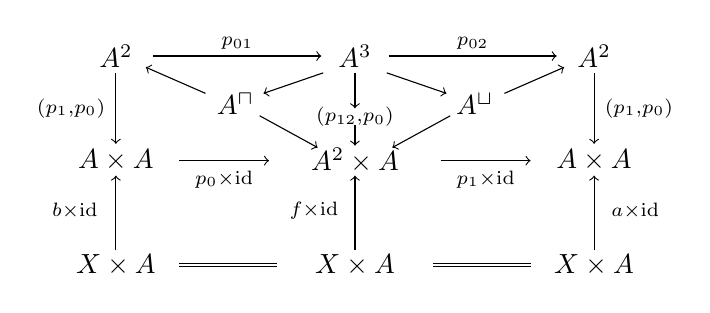
\begin{tikzpicture}[x=1.35em,y=1.35em]
  \node (A2l) at (-6.4,3.2) {$A^{2}$};
  \node (A3) at (0,3.2) {$A^{3}$};
  \node (A2r) at (6.4,3.2) {$A^{2}$};
  \node (Asp) at (-3.2,1.9) {$A^{\ShapeSpan}$};
  \node (Acsp) at (3.2,1.9) {$A^{\ShapeCospan}$};
  \node (AAl) at (-6.4,0.4) {$A\times A$};
  \node (AAm) at (0,0.4) {$A^{2}\times A$};
  \node (AAr) at (6.4,0.4) {$A\times A$};
  \node (XAl) at (-6.4,-2.4) {$X\times A$};
  \node (XAm) at (0,-2.4) {$X\times A$};
  \node (XAr) at (6.4,-2.4) {$X\times A$};
  \draw[->] (-5.4,3.2) -- (-0.9,3.2);
  \node at (-3.15,3.55) {$\scriptstyle p_{01}$};
  \draw[->] (0.9,3.2) -- (5.4,3.2);
  \node at (3.15,3.55) {$\scriptstyle p_{02}$};
  \draw[->] (-0.85,2.75) -- (-2.45,2.2);
  \draw[->] (0.85,2.75) -- (2.45,2.2);
  \draw[->] (-4.0,2.2) -- (-5.6,2.9);
  \draw[->] (4.0,2.2) -- (5.6,2.9);
  \draw[->] (-2.55,1.6) -- (-1.0,0.75);
  \draw[->] (2.55,1.6) -- (1.0,0.75);
  \draw[->] (0,2.75) -- (0,1.8);
  \draw[->] (0,1.35) -- (0,0.8);
  \node at (0,1.58) {$\scriptstyle(p_{12},p_{0})$};
  \node at (-3.9,1.4) {$\scriptstyle\lrcorner$};
  \node at (3.9,1.4) {$\scriptstyle\lrcorner$};
  \draw[->] (-6.4,2.75) -- (-6.4,0.85);
  \node at (-7.6,1.8) {$\scriptstyle(p_{1},p_{0})$};
  \draw[->] (6.4,2.75) -- (6.4,0.85);
  \node at (7.6,1.8) {$\scriptstyle(p_{1},p_{0})$};
  \draw[->] (-4.7,0.4) -- (-2.3,0.4);
  \node at (-3.5,-0.1) {$\scriptstyle p_{0}\times\mathrm{id}$};
  \draw[->] (2.3,0.4) -- (4.7,0.4);
  \node at (3.5,-0.1) {$\scriptstyle p_{1}\times\mathrm{id}$};
  \draw[->] (-6.4,-2.0) -- (-6.4,0.0);
  \node at (-7.5,-0.95) {$\scriptstyle b\times\mathrm{id}$};
  \draw[->] (0,-2.0) -- (0,0.0);
  \node at (-1.1,-0.95) {$\scriptstyle f\times\mathrm{id}$};
  \draw[->] (6.4,-2.0) -- (6.4,0.0);
  \node at (7.5,-0.95) {$\scriptstyle a\times\mathrm{id}$};
  \draw[double] (-4.7,-2.4) -- (-2.1,-2.4);
  \draw[double] (2.1,-2.4) -- (4.7,-2.4);
\end{tikzpicture}
\end{center}
注意，上方两个方块中到诸拉回的映射分别定义出一个平凡纤维化与一个等价纤维化。
于是，依命题 C.1.12，诱导映射
$p_{01}\colon A_{/f}\twoheadrightarrow\mathrm{Hom}_{A}(A,b)$ 是一个平凡纤维化，
而诱导映射 $p_{02}\colon A_{/f}\twoheadrightarrow\mathrm{Hom}_{A}(A,a)$ 是一个
等价纤维化。
特别地，从下方左侧的诸拉回可见：到平凡纤维化 $p_{01}$ 的那些截面，对应于把
可复合箭头对 $\phi\colon\mathrm{Hom}_{A}(A,b)\to A^{2}$ 与
$fp_{1}\colon\mathrm{Hom}_{A}(A,b)\to A^{2}$ 扩充为
$\mathrm{Fun}(\mathrm{Hom}_{A}(A,b),A)$ 中某个 $2$-单纯形的那些映射
$\mathrm{Hom}_{A}(A,b)\to A^{3}$：
\begin{center}
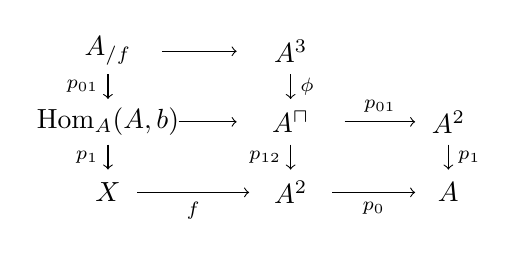
\begin{tikzpicture}[x=1.5em,y=1.5em]
  \node (Af) at (0,3.4) {$A_{/f}$};
  \node (A3t) at (4.4,3.4) {$A^{3}$};
  \node (Hb) at (0,1.7) {$\mathrm{Hom}_{A}(A,b)$};
  \node (Acap) at (4.4,1.7) {$A^{\ShapeSpan}$};
  \node (A2m) at (8.2,1.7) {$A^{2}$};
  \node (X) at (0,0) {$X$};
  \node (A2b) at (4.4,0) {$A^{2}$};
  \node (Ab) at (8.2,0) {$A$};
  \draw[->] (1.3,3.4) -- (3.1,3.4);
  \node at (1.6,2.4) {$\scriptstyle\lrcorner$};
  \draw[->] (0,2.85) -- node[left]{$\scriptstyle p_{01}$} (0,2.25);
  \draw[->] (4.4,2.85) -- node[right]{$\scriptstyle\phi$} (4.4,2.25);
  \draw[->] (1.7,1.7) -- (3.1,1.7);
  \draw[->] (5.7,1.7) -- node[above]{$\scriptstyle p_{01}$} (7.4,1.7);
  \draw[->] (4.4,1.15) -- node[left]{$\scriptstyle p_{12}$} (4.4,0.55);
  \node at (6.2,0.7) {$\scriptstyle\lrcorner$};
  \draw[->] (8.2,1.15) -- node[right]{$\scriptstyle p_{1}$} (8.2,0.55);
  \draw[->] (0,1.15) -- node[left]{$\scriptstyle p_{1}$} (0,0.55);%
  \draw[->] (0.7,0) -- node[below]{$\scriptstyle f$} (3.4,0);
  \draw[->] (5.4,0) -- node[below]{$\scriptstyle p_{0}$} (7.4,0);
\end{tikzpicture}
\qquad
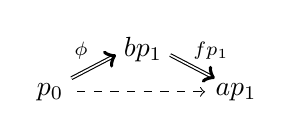
\begin{tikzpicture}[x=1.4em,y=1.4em]
  \node (p0) at (0,0) {$p_{0}$};
  \node (bp1) at (2.4,1.1) {$bp_{1}$};
  \node (ap1) at (4.8,0) {$ap_{1}$};
  \draw[->,double] (0.55,0.35) -- (1.7,0.95);
  \node at (0.8,1.05) {$\scriptstyle\phi$};
  \draw[->,double] (3.1,0.95) -- (4.25,0.35);
  \node at (4.15,1.05) {$\scriptstyle fp_{1}$};
  \draw[->,dashed] (0.7,0) -- (4.0,0);
\end{tikzpicture}
\end{center}
类似地，拉回
\begin{center}
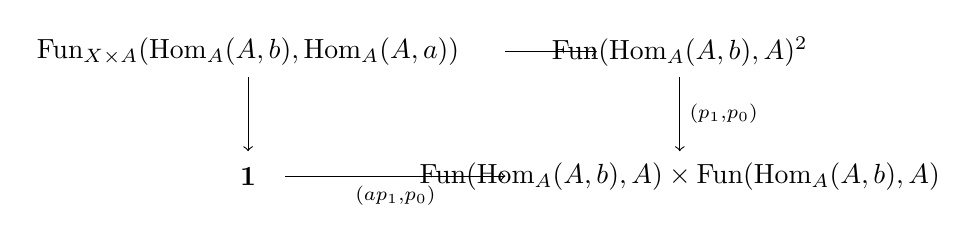
\begin{tikzpicture}[x=1.5em,y=1.5em]
  \node (tl) at (0,1.5) {$\mathrm{Fun}_{X\times A}(\mathrm{Hom}_{A}(A,b),\mathrm{Hom}_{A}(A,a))$};
  \node (tr) at (10.4,1.5) {$\mathrm{Fun}(\mathrm{Hom}_{A}(A,b),A)^{2}$};
  \node (bl) at (0,-1.5) {$\qcOne$};
  \node (br) at (10.4,-1.5) {$\mathrm{Fun}(\mathrm{Hom}_{A}(A,b),A)\times\mathrm{Fun}(\mathrm{Hom}_{A}(A,b),A)$};
  \draw[->] (6.2,1.5) -- (8.4,1.5);
  \draw[->] (0,0.9) -- (0,-0.9);
  \node at (1.4,0) {$\scriptstyle\lrcorner$};
  \draw[->] (10.4,0.9) -- node[right]{$\scriptstyle(p_{1},p_{0})$} (10.4,-0.9);
  \draw[->] (0.9,-1.5) -- node[below]{$\scriptstyle(ap_{1},p_{0})$} (6.2,-1.5);
\end{tikzpicture}
\end{center}
表明：函子 $f_{*}\colon\mathrm{Hom}_{A}(A,b)\to\mathrm{Hom}_{A}(A,a)$ 对应于为
复合箭头选取代表 $fp_{1}\cdot\phi\colon\mathrm{Hom}_{A}(A,b)\to A^{2}$（与推论
3.5.11 的证明比较）。于是，每个截面都在函子的正确\trFiberedIsomorphism{}类中
定义出一个映射；反之，由于 $\mathrm{hFun}(\mathrm{Hom}_{A}(A,b),A)$ 中定义交换
图的每组三元箭头都在 $\mathrm{Fun}(\mathrm{Hom}_{A}(A,b),A)$ 中界定出某个
$2$-单纯形（见引理 1.1.12），每个表示性的函子都按此方式产生。

最后，依练习 3.6.ii 与推论 3.5.11：$f\colon b\Rightarrow a$ 是同构，当且仅当函子
\allowbreak$f_{*}\colon\mathrm{Hom}_{A}(A,b)\to\allowbreak\mathrm{Hom}_{A}(A,a)$
是一个\trFiberedEquivalence{}；而由\trTwoOfThreeProperty{}，$f$ 是同构，当且仅当
$p_{02}$ 是一个平凡纤维化。
\end{proof}

\begin{lemma}[作为绝对提升图的拉回方块]\label{lem:pullbacks-as-absolute-liftings}
\trInfinityCategory{} $A$ 中的一个交换方块是一个拉回方块，当且仅当其诱导的自然变换
$(\mathrm{id}_{a},v)$ 构成一个绝对右提升图表
\begin{center}
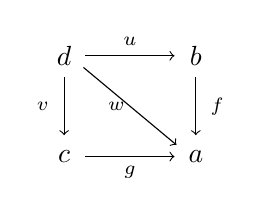
\begin{tikzpicture}[x=1.4em,y=1.4em]
  \node (d) at (0,1.7) {$d$};
  \node (b) at (3.4,1.7) {$b$};
  \node (c) at (0,-0.9) {$c$};
  \node (a) at (3.4,-0.9) {$a$};
  \draw[->] (0.55,1.7) -- (2.85,1.7);
  \node at (1.7,2.08) {$\scriptstyle u$};
  \draw[->] (0,1.15) -- (0,-0.35);
  \node at (-0.55,0.4) {$\scriptstyle v$};
  \draw[->] (3.4,1.15) -- (3.4,-0.35);
  \node at (3.95,0.4) {$\scriptstyle f$};
  \draw[->] (0.55,-0.9) -- (2.85,-0.9);
  \node at (1.7,-1.3) {$\scriptstyle g$};
  \draw[->] (0.5,1.4) -- (2.9,-0.6);
  \node at (1.35,0.4) {$\scriptstyle w$};
\end{tikzpicture}
\qquad
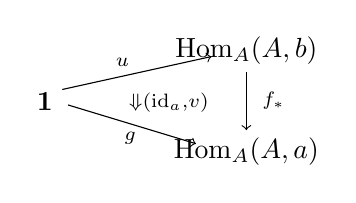
\begin{tikzpicture}[x=1.4em,y=1.4em]
  \node (Hb) at (5.2,1.7) {$\mathrm{Hom}_{A}(A,b)$};
  \node (One) at (0,0.4) {$\qcOne$};
  \node (Ha) at (5.2,-0.9) {$\mathrm{Hom}_{A}(A,a)$};
  \draw[->] (0.45,0.7) -- (4.3,1.55);
  \node at (2.0,1.4) {$\scriptstyle u$};
  \node at (3.2,0.35) {$\scriptstyle\Downarrow(\mathrm{id}_{a},v)$};
  \draw[->] (5.2,1.15) -- (5.2,-0.35);
  \node at (5.9,0.4) {$\scriptstyle f_{*}$};
  \draw[->] (0.6,0.3) -- (3.9,-0.7);
  \node at (2.2,-0.55) {$\scriptstyle g$};
\end{tikzpicture}
\end{center}
\end{lemma}

该陈述需要一些解释。\trInfinityCategory{} $A$ 中的一个交换方块
$s\colon\qcOne\to A^{\ShapeSquare}$ 定义了 $\mathrm{Fun}(\qcOne,A)^{\ShapeSquare}$
的一个元素，其数据由四个顶点 $d$、$b$、$c$、$a\colon\qcOne\to A$ 与五个 $1$-单纯形
$u$、$v$、$f$、$g$、$w\colon\qcOne\to A^{2}$ 给出——它们位于 $A$ 的%
\trUnderlyingQuasiCategory{} $A_{0}:=\mathrm{Fun}(\qcOne,A)$ 之中，如上左图所示
——连同未命名的一对 $2$-单纯形，后者在 $\mathrm{h}A:=\mathrm{hFun}(\qcOne,A)$ 中
见证交换性 $fu=w=gv$。依命题 3.4.7，复合 $f_{*}u$ 同构于 $fu$。依%
\trTwoCellInduction{}，如上右图所示的自然变换 $(\mathrm{id}_{a},v)\colon fu\Rightarrow g$
可通过指明其定义域与余定义域分量来构造，前者我们取为 $v\colon d\Rightarrow c$，
后者我们取为 $\mathrm{id}_{a}$。

\begin{proof}
依推论 4.2.8，限制函子
\begin{center}
\begin{tikzpicture}[x=1.5em,y=1.5em]
  \node (tl) at (0,1.5) {$A^{\ShapeSquare}_{g\vee f}$};
  \node (tr) at (5.4,1.5) {$A^{\ShapeSquare}$};
  \node (bl) at (0,-1.5) {$\qcOne$};
  \node (br) at (5.4,-1.5) {$A^{\ShapeCospan}$};
  \draw[->] (1.75,1.5) -- (3.9,1.5);
  \draw[->] (0,0.9) -- (0,-0.9);
  \node at (1.5,0.1) {$\scriptstyle\lrcorner$};
  \draw[->] (5.4,0.9) -- node[right]{$\scriptstyle\mathrm{res}$} (5.4,-0.9);
  \draw[->] (1.0,-1.5) -- node[below]{$\scriptstyle g\vee f$} (4.5,-1.5);
\end{tikzpicture}
\end{center}
的\trFiber{}等价于余跨度图 $g\vee f$ 之上的\trInfinityCategoryOfCones{}。依%
\cref{prop:limits-as-terminal-cones}，要证明交换方块定义一个拉回图，就是要证明
$(v,f,u,g)\colon\qcOne\to A^{\ShapeSquare}_{g\vee f}$ 定义一个\trTerminal{}\trElement{}。
类似地，依推论 3.6.10，二元组 $(u,(\mathrm{id}_{a},v))$ 定义一个绝对右提升图表，
当且仅当它在逗号∞-范畴 $\mathrm{Hom}_{\mathrm{Hom}_{A}(A,a)}(f_{*},g)$ 中表示一个%
\trTerminal{}\trElement{}。我们宣称：$A^{\ShapeSquare}_{g\vee f}$ 与
$\mathrm{Hom}_{\mathrm{Hom}_{A}(A,a)}(f_{*},g)$ 经由识别这些元素的映射而%
\trEquivalence{}，这就证明了双条件。

为看出这一点，注意单纯方块 $\ShapeSquare$ 可以由沿其对角边粘合两个 $2$-单纯形
而构成，这就给出左下方的拉回：
\begin{center}
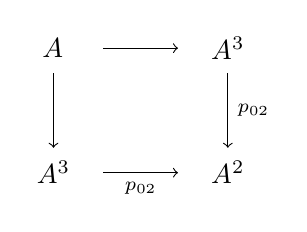
\begin{tikzpicture}[x=1.5em,y=1.5em]
  \node (tl) at (0,1.5) {$A^{\ShapeSquare}$};
  \node (tr) at (4.2,1.5) {$A^{3}$};
  \node (bl) at (0,-1.5) {$A^{3}$};
  \node (br) at (4.2,-1.5) {$A^{2}$};
  \draw[->] (1.2,1.5) -- (3.0,1.5);
  \draw[->] (0,0.9) -- (0,-0.9);
  \node at (1.4,0.1) {$\scriptstyle\lrcorner$};
  \draw[->] (4.2,0.9) -- node[right]{$\scriptstyle p_{02}$} (4.2,-0.9);
  \draw[->] (1.2,-1.5) -- node[below]{$\scriptstyle p_{02}$} (3.0,-1.5);
\end{tikzpicture}
\qquad
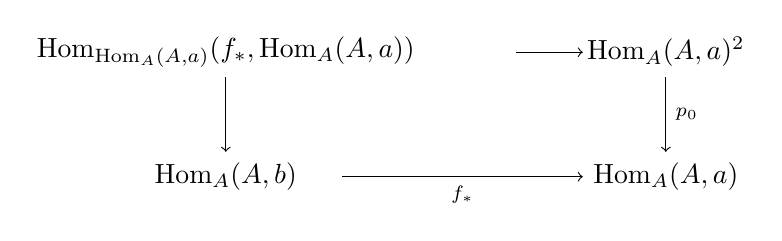
\begin{tikzpicture}[x=1.5em,y=1.5em]
  \node (tl) at (0,1.5) {$\mathrm{Hom}_{\mathrm{Hom}_{A}(A,a)}(f_{*},\mathrm{Hom}_{A}(A,a))$};
  \node (tr) at (10.6,1.5) {$\mathrm{Hom}_{A}(A,a)^{2}$};
  \node (bl) at (0,-1.5) {$\mathrm{Hom}_{A}(A,b)$};
  \node (br) at (10.6,-1.5) {$\mathrm{Hom}_{A}(A,a)$};
  \draw[->] (7.0,1.5) -- (8.6,1.5);
  \draw[->] (0,0.9) -- (0,-0.9);
  \node at (1.7,0.1) {$\scriptstyle\lrcorner$};
  \draw[->] (10.6,0.9) -- node[right]{$\scriptstyle p_{0}$} (10.6,-0.9);
  \draw[->] (2.8,-1.5) -- node[below]{$\scriptstyle f_{*}$} (8.6,-1.5);
\end{tikzpicture}
\end{center}
我们论证：其拉回定义出上方右侧所展示的逗号∞-范畴的那个余跨度中的诸映射，各自
等价于函子 $p_{02}\colon A^{3}\to A^{2}$ 到适当\trFiber{}上的诸拉回。依%
\cref{lem:postcomposition}，映射 $p_{02}\colon A^{3}\to A^{2}$ 在 $f$ 与 $a$ 之上
的诸\trFiber{}上分别拉回到一个等价于 $f_{*}$ 的映射，故只需考虑映射 $p_{0}$。

对定义 $\mathrm{Hom}_{A}(A,a)$ 的拉回图应用 $(-)^{2}$，便得到一个可分解为两个
拉回之复合的拉回方块：
\begin{center}
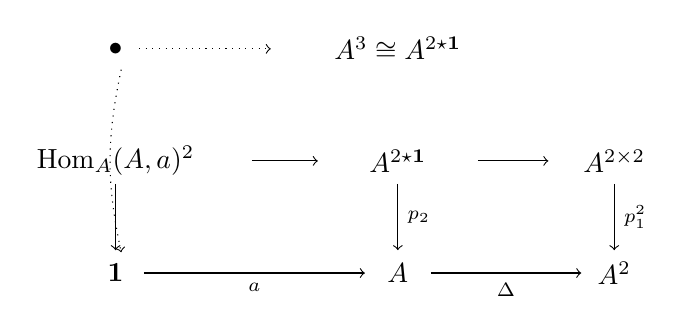
\begin{tikzpicture}[x=1.7em,y=1.5em]
  \node (dot) at (0,2.7) {$\bullet$};
  \node (A3t) at (6.0,2.7) {$A^{3}\cong A^{2\star\qcOne}$};
  \node (Hom2) at (0,0) {$\mathrm{Hom}_{A}(A,a)^{2}$};
  \node (Ast) at (6.0,0) {$A^{2\star\qcOne}$};
  \node (Asq2) at (10.6,0) {$A^{2\times 2}$};
  \node (One) at (0,-2.7) {$\qcOne$};
  \node (A) at (6.0,-2.7) {$A$};
  \node (A2) at (10.6,-2.7) {$A^{2}$};
  \draw[->,dotted] (0.5,2.7) -- (3.3,2.7);
  \draw[->,dotted] (0.12,2.2) to[bend right=12] (0.12,-2.2);
  \draw[->] (2.9,0) -- (4.3,0);
  \draw[->] (7.7,0) -- (9.2,0);
  \draw[->] (0,-0.55) -- (0,-2.15);
  \node at (1.5,-0.75) {$\scriptstyle\lrcorner$};
  \draw[->] (6.0,-0.55) -- node[right]{$\scriptstyle p_{2}$} (6.0,-2.15);
  \node at (8.0,-0.75) {$\scriptstyle\lrcorner$};
  \draw[->] (10.6,-0.55) -- node[right]{$\scriptstyle p_{1}^{2}$} (10.6,-2.15);
  \draw[->] (0.6,-2.7) -- node[below]{$\scriptstyle a$} (5.3,-2.7);
  \draw[->] (6.7,-2.7) -- node[below]{$\scriptstyle\Delta$} (9.9,-2.7);
\end{tikzpicture}
\end{center}
依命题 4.2.7 的等价 $A^{2\star\qcOne}\simeq A^{2\diamond\qcOne}$，左边的拉回方块
表明 $\mathrm{Hom}_{A}(A,a)^{2}$ 等价于 $p_{2}\colon A^{3}\to A$ 沿
$a\colon\qcOne\to A$ 的\trFiber{}。模去这一等价，定义域投影映射
$p_{0}\colon\mathrm{Hom}_{A}(A,a)^{2}\to\mathrm{Hom}_{A}(A,a)$ 等价于由
\begin{center}
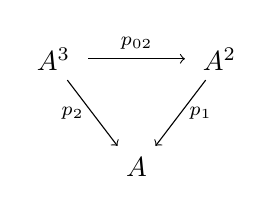
\begin{tikzpicture}[x=1.25em,y=1.4em]
  \node (A3) at (0,1.5) {$A^{3}$};
  \node (A2) at (4.8,1.5) {$A^{2}$};
  \node (A) at (2.4,-1.3) {$A$};
  \draw[->] (1.0,1.5) -- node[above]{$\scriptstyle p_{02}$} (3.8,1.5);
  \draw[->] (0.4,0.95) -- (1.85,-0.75);
  \node at (0.55,0.1) {$\scriptstyle p_{2}$};
  \draw[->] (4.4,0.95) -- (2.95,-0.75);
  \node at (4.25,0.1) {$\scriptstyle p_{1}$};
\end{tikzpicture}
\end{center}
在 $a\colon\qcOne\to A$ 之上的诸\trFiber{}上诱导的映射。余定义域投影
$p_{1}\colon\mathrm{Hom}_{A}(A,a)^{2}\to\mathrm{Hom}_{A}(A,a)$ 类似地等价于%
\trFibered{}投影映射 $p_{12}\colon A^{3}\to A^{2}$ 沿 $a\colon\qcOne\to A$ 的拉回。

把这些拼在一起，逗号∞-范畴
$\mathrm{Hom}_{\mathrm{Hom}_{A}(A,a)}(f_{*},\mathrm{Hom}_{A}(A,a))$ 便等价于下图
之极限：
\begin{center}
\begin{tikzpicture}[x=1.6em,y=1.6em]
  \node (dot) at (0,0) {$\bullet$};
  \node (Asq) at (3.0,0) {$A^{\ShapeSquare}$};
  \node (A3) at (6.0,0) {$A^{3}$};
  \node (A2t) at (9.4,0) {$A^{2}$};
  \node (A3m) at (3.0,-2.3) {$A^{3}$};
  \node (A2m) at (6.0,-2.3) {$A^{2}$};
  \node (One) at (0,-4.6) {$\qcOne$};
  \node (A2b) at (3.0,-4.6) {$A^{2}$};
  \draw[->] (0.5,0) -- (2.1,0);
  \draw[->] (3.9,0) -- (5.1,0);
  \draw[->] (6.9,0) -- node[above]{$\scriptstyle p_{12}$} (8.5,0);
  \draw[->] (0,-0.55) -- (0,-4.05);
  \draw[->] (3.0,-0.55) -- (3.0,-1.75);
  \draw[->] (6.0,-0.55) -- node[right]{$\scriptstyle p_{02}$} (6.0,-1.75);
  \node at (1.55,-0.75) {$\scriptstyle\lrcorner$};
  \node at (4.55,-0.75) {$\scriptstyle\lrcorner$};
  \draw[->] (3.9,-2.3) -- node[above]{$\scriptstyle p_{02}$} (5.1,-2.3);
  \draw[->] (3.0,-2.85) -- node[left]{$\scriptstyle p_{12}$} (3.0,-4.05);
  \draw[->] (0.55,-4.6) -- node[below]{$\scriptstyle f$} (2.1,-4.6);
\end{tikzpicture}
\end{center}
余定义域投影
$p_{1}\colon\mathrm{Hom}_{\mathrm{Hom}_{A}(A,a)}(f_{*},\mathrm{Hom}_{A}(A,a))\to\mathrm{Hom}_{A}(A,a)$
是上图顶部水平复合沿包含 $\mathrm{Hom}_{A}(A,a)\to A^{2}$ 的拉回。于是，逗号
∞-范畴 $\mathrm{Hom}_{\mathrm{Hom}_{A}(A,a)}(f_{*},g)$ 等价于左下方的极限，后者
重排为定义\trFiber{} $A^{\ShapeSquare}_{g\vee f}$ 的右下方拉回，这就证明了所宣称
的等价：
\begin{center}
\begin{tikzpicture}[x=1.6em,y=1.6em]
  \node (dot1) at (0,2.3) {$\bullet$};
  \node (dot2) at (3.0,2.3) {$\bullet$};
  \node (Onet) at (9.4,2.3) {$\qcOne$};
  \node (dotb) at (0,0) {$\bullet$};
  \node (Asq) at (3.0,0) {$A^{\ShapeSquare}$};
  \node (A3) at (6.0,0) {$A^{3}$};
  \node (A2t) at (9.4,0) {$A^{2}$};
  \node (A3m) at (3.0,-2.3) {$A^{3}$};
  \node (A2m) at (6.0,-2.3) {$A^{2}$};
  \node (One) at (0,-4.6) {$\qcOne$};
  \node (A2b) at (3.0,-4.6) {$A^{2}$};
  \draw[->] (0.5,2.3) -- (2.1,2.3);
  \draw[->] (3.9,2.3) -- (8.5,2.3);
  \draw[->] (9.4,1.75) -- node[right]{$\scriptstyle g$} (9.4,0.55);
  \draw[->] (0.5,0) -- (2.1,0);
  \draw[->] (3.9,0) -- (5.1,0);
  \draw[->] (6.9,0) -- node[above]{$\scriptstyle p_{12}$} (8.5,0);
  \draw[->] (0,-0.55) -- (0,-4.05);
  \draw[->] (3.0,-0.55) -- (3.0,-1.75);
  \draw[->] (6.0,-0.55) -- node[right]{$\scriptstyle p_{02}$} (6.0,-1.75);
  \node at (1.55,-0.75) {$\scriptstyle\lrcorner$};
  \node at (4.55,-0.75) {$\scriptstyle\lrcorner$};
  \draw[->] (3.9,-2.3) -- node[above]{$\scriptstyle p_{02}$} (5.1,-2.3);
  \draw[->] (3.0,-2.85) -- node[left]{$\scriptstyle p_{12}$} (3.0,-4.05);
  \draw[->] (0.55,-4.6) -- node[below]{$\scriptstyle f$} (2.1,-4.6);
\end{tikzpicture}
\qquad
\begin{tikzpicture}[x=1.5em,y=1.5em]
  \node (tl) at (0,1.5) {$A^{\ShapeSquare}_{g\vee f}$};
  \node (tr) at (5.4,1.5) {$A^{\ShapeSquare}$};
  \node (bl) at (0,-1.5) {$\qcOne$};
  \node (br) at (5.4,-1.5) {$A^{\ShapeCospan}$};
  \draw[->] (1.75,1.5) -- (3.9,1.5);
  \draw[->] (0,0.9) -- (0,-0.9);
  \node at (1.5,0.1) {$\scriptstyle\lrcorner$};
  \draw[->] (5.4,0.9) -- node[right]{$\scriptstyle\mathrm{res}$} (5.4,-0.9);
  \draw[->] (1.0,-1.5) -- node[below]{$\scriptstyle g\vee f$} (4.5,-1.5);
\end{tikzpicture}
\end{center}
\end{proof}

单纯集 $2\times2$ 有一个非恒同的自同构，它诱导 $A^{\ShapeSquare}$ 的一个
「转置」自同构。由对称性，$A$ 中的一个交换方块是拉回方块，当且仅当其转置方块是
拉回方块。这给出\cref{lem:pullbacks-as-absolute-liftings}的一个对偶形式，其中
$f$ 与 $g$ 的角色以及 $u$ 与 $v$ 的角色互换。作为推论，我们可以轻松证明：拉回
方块既可「竖直」复合又可「水平」复合，并且可以从「右边」与「底部」消去。

\begin{proposition}[拉回方块的复合与消去]\label{prop:pullback-square-cancelation}
给定 $A$ 中一个可复合的交换方块对及其复合矩形——后者经由等价
$A^{3\times 2}\simeq A^{\ShapeSquare}\times_{A^{2}}A^{\ShapeSquare}$ 定义——
\begin{center}
\begin{tikzpicture}[x=1.4em,y=1.4em]
  \node (p) at (0,1.8) {$p$};
  \node (d) at (3.6,1.8) {$d$};
  \node (b) at (7.2,1.8) {$b$};
  \node (e) at (0,-1.2) {$e$};
  \node (c) at (3.6,-1.2) {$c$};
  \node (a) at (7.2,-1.2) {$a$};
  \draw[->] (0.5,1.8) -- node[above]{$\scriptstyle x$} (3.1,1.8);
  \draw[->] (4.1,1.8) -- node[above]{$\scriptstyle u$} (6.7,1.8);
  \draw[->] (0,1.25) -- node[left]{$\scriptstyle y$} (0,-0.65);
  \draw[->] (3.6,1.25) -- node[left]{$\scriptstyle v$} (3.6,-0.65);
  \draw[->] (7.2,1.25) -- node[right]{$\scriptstyle f$} (7.2,-0.65);
  \draw[->] (0.5,-1.2) -- node[below]{$\scriptstyle h$} (3.1,-1.2);
  \draw[->] (4.1,-1.2) -- node[below]{$\scriptstyle g$} (6.7,-1.2);
  \draw[->] (0.45,1.5) -- node[pos=0.3,below left]{$\scriptstyle z$} (3.15,-0.9);
  \draw[->] (4.05,1.5) -- node[pos=0.3,below left]{$\scriptstyle w$} (6.75,-0.9);
\end{tikzpicture}
\end{center}
若右边的方块是拉回方块，则左边的方块是拉回方块，当且仅当复合矩形是拉回方块。
\end{proposition}

\begin{proof}
依\cref{lem:pullbacks-as-absolute-liftings}，我们给定一个绝对右提升图表
\begin{center}
\begin{tikzpicture}[x=1.4em,y=1.4em]
  \node (Hc) at (5.2,1.7) {$\mathrm{Hom}_{A}(A,c)$};
  \node (One) at (0,0.4) {$\qcOne$};
  \node (Ha) at (5.2,-0.9) {$\mathrm{Hom}_{A}(A,a)$};
  \draw[->] (0.45,0.7) -- (4.3,1.55);
  \node at (2.0,1.4) {$\scriptstyle v$};
  \node at (3.2,0.35) {$\scriptstyle\Downarrow(\mathrm{id}_{a},u)$};
  \draw[->] (5.2,1.15) -- (5.2,-0.35);
  \node at (5.9,0.4) {$\scriptstyle g_{*}$};
  \draw[->] (0.6,0.3) -- (3.9,-0.7);
  \node at (2.2,-0.55) {$\scriptstyle f$};
\end{tikzpicture}
\end{center}
依引理 2.4.1，复合图
\begin{center}
\begin{tikzpicture}[x=1.4em,y=1.4em]
  \node (He) at (5.2,3.4) {$\mathrm{Hom}_{A}(A,e)$};
  \node (Hc) at (5.2,1.1) {$\mathrm{Hom}_{A}(A,c)$};
  \node (Ha) at (5.2,-1.6) {$\mathrm{Hom}_{A}(A,a)$};
  \node (One) at (0,0.9) {$\qcOne$};
  \draw[->] (0.5,1.25) to[bend left=14] (4.5,3.2);
  \node at (1.5,2.75) {$\scriptstyle y$};
  \node at (3.3,1.95) {$\scriptstyle\Downarrow(\mathrm{id}_{c},x)$};
  \draw[->] (5.2,2.85) -- (5.2,1.65);
  \node at (5.9,2.25) {$\scriptstyle h_{*}$};
  \draw[->] (0.45,0.95) -- (4.3,1.25);
  \node at (2.2,1.42) {$\scriptstyle v$};
  \node at (3.3,0.15) {$\scriptstyle\Downarrow(\mathrm{id}_{a},u)$};
  \draw[->] (5.2,0.55) -- (5.2,-1.05);
  \node at (5.9,-0.25) {$\scriptstyle g_{*}$};
  \draw[->] (0.6,0.7) -- (3.9,-1.4);
  \node at (2.2,-0.7) {$\scriptstyle f$};
\end{tikzpicture}
\end{center}
是一个绝对右提升图表，当且仅当顶部的三角是绝对右提升图表。依%
\cref{lem:pullbacks-as-absolute-liftings}，这正是所要证明的。
\end{proof}

\begin{remark}\label{rem:x-indexed-pullback-squares}
\cref{prop:pullback-square-cancelation}的结果对 $X$-索引的交换方块族同样成立，
后者指\trDiagram{} $X\to A^{\ShapeSquare}$，或等价地，
$\mathrm{Fun}(X,A)^{\ShapeSquare}$ 的诸元素。证明相同，它利用%
\cref{lem:pullbacks-as-absolute-liftings}的一个推广：该推广断言，∞-宇宙
$\mathcal{K}$ 中取值于\trInfinityCategory{} $A$ 的、如下左图所示的 $X$-索引交换
方块是拉回方块，当且仅当如下右图所诱导的 2-胞腔 $(\mathrm{id}_{a},v)$ 是
$\mathcal{K}_{/X}$ 中的一个绝对右提升图表：
\begin{center}
\begin{tikzpicture}[x=1.4em,y=1.4em]
  \node (d) at (0,1.7) {$d$};
  \node (b) at (3.4,1.7) {$b$};
  \node (c) at (0,-0.9) {$c$};
  \node (a) at (3.4,-0.9) {$a$};
  \draw[->] (0.55,1.7) -- node[above]{$\scriptstyle u$} (2.85,1.7);
  \draw[->] (0,1.15) -- node[left]{$\scriptstyle v$} (0,-0.35);
  \draw[->] (3.4,1.15) -- node[right]{$\scriptstyle f$} (3.4,-0.35);
  \draw[->] (0.55,-0.9) -- node[below]{$\scriptstyle g$} (2.85,-0.9);
  \draw[->] (0.5,1.4) -- node[pos=0.3,below left]{$\scriptstyle w$} (2.9,-0.6);
\end{tikzpicture}
\qquad
\begin{tikzpicture}[x=1.4em,y=1.4em]
  \node (Hb) at (5.6,1.9) {$\mathrm{Hom}_{A}(A,b)$};
  \node (Xm) at (0,0.4) {$X$};
  \node (Ha) at (5.6,-0.8) {$\mathrm{Hom}_{A}(A,a)$};
  \node (Xb) at (2.4,-2.4) {$X$};
  \draw[->] (0.5,0.7) -- (4.7,1.7);
  \node at (2.2,1.45) {$\scriptstyle u$};
  \node at (3.3,0.45) {$\scriptstyle\Downarrow(\mathrm{id}_{a},v)$};
  \draw[->] (5.6,1.35) -- (5.6,-0.25);
  \node at (6.3,0.55) {$\scriptstyle f_{*}$};
  \draw[->] (0.65,0.3) -- (4.3,-0.55);
  \node at (2.5,-0.4) {$\scriptstyle g$};
  \draw[->,dotted] (0.3,0.0) -- (2.0,-2.1);
  \node at (0.5,-1.2) {$\scriptstyle p_{1}$};
  \draw[->,dotted] (2.9,-2.2) -- (4.9,-1.15);
  \node at (4.1,-1.95) {$\scriptstyle p_{1}$};
\end{tikzpicture}
\end{center}
\end{remark}

对 $X$-索引拉回方块的这一刻画，可以通过在切片∞-宇宙 $\mathcal{K}_{/X}$ 中重新
实现\cref{lem:pullbacks-as-absolute-liftings}之证明所给的构造来证明——以逗号
∞-范畴与切片∞-宇宙 $\mathcal{K}_{/X}$ 中的单纯极限（如命题 1.2.22 所描述者）取代
$\mathcal{K}$ 中的类似构造。若非涉及的记号更为繁复，我们本会呈现这个一般证明而非
上面的特殊情形。

另一种做法是，这一扩展可以从我们在此证明的结果推导出来。$\mathcal{K}$ 中的一个%
\trDiagram{} $s\colon X\to A^{\ShapeSquare}$ 也定义了切片∞-宇宙 $\mathcal{K}_{/X}$
中以 $\pi\colon A\times X\to X$ 为取值的一个 $X$-索引交换方块，其形式为 $X$ 之上的
一个函子 $(s,\mathrm{id}_{X})\colon X\to A^{\ShapeSquare}\times X$。容易验证：
取值于 $\pi\colon A\times X\to X$ 且其在 $X$ 处的分量为恒同的\trDiagram{}在
$\mathcal{K}_{/X}$ 中有\trLimit{}，当且仅当该\trDiagram{}的 $A$ 分量在 $\mathcal{K}$
中有\trLimit{}。由于 $\mathrm{id}_{X}$ 是 $\mathcal{K}_{/X}$ 的\trTerminal{}对象，
这个对象就是 $\mathcal{K}_{/X}$ 中的∞-范畴 $1$，故%
\cref{lem:pullbacks-as-absolute-liftings}在切片∞-宇宙 $\mathcal{K}_{/X}$ 中适用，
从而证明了 $\mathcal{K}$ 中 $X$-索引交换方块族的一般情形。

正如例 2.3.10 所讨论的，\trTerminal{}\trElement{}与\trInitial{}\trElement{}分别
是\trLimit{}与\trColimit{}的特殊情形，其中\trDiagram{}形状为空。
对任何\trInfinityCategory{} $A$，$A$ 中诸\trEmptyDiagram{}的∞-范畴
$A^{\emptyset}\cong\qcOne$ 是\trTerminal{}的。于是，$A$ 中存在唯一的
$\emptyset$-索引\trDiagram{}。由定义 4.2.1 中逗号∞-范畴的构造立即可知：唯一空%
\trDiagram{}之上与之下二者的\trInfinityCategoryOfCones{}都同构于 $A$。
在空\trDiagram{}之上的\trCone{}的情形，把\trCone{}送到其顶点的定义域求值函子在
$A$ 上是恒同；而在空\trDiagram{}之下的\trCone{}的情形，把\trCone{}送到其\trNadir{}的
余定义域求值函子在 $A$ 上是恒同。
下面这个关于\trTerminal{}\trElement{}的刻画可以当作%
\cref{prop:colimits-represent-cones}的特殊情形推导出来，不过我们发现从命题 4.1.1
出发论证更为容易。

\begin{proposition}\label{prop:terminal-initial-trivial-fibration}
\trInfinityCategory{} $A$ 的一个\trElement{} $a\colon\qcOne\to A$
(i) 定义 $A$ 的一个\trTerminal{}\trElement{}，当且仅当定义域投影函子
$p_{0}\colon\mathrm{Hom}_{A}(A,a)\twoheadrightarrow A$ 是一个平凡纤维化；而
(ii) 定义 $A$ 的一个\trInitial{}\trElement{}，当且仅当余定义域投影函子
$p_{1}\colon\mathrm{Hom}_{A}(a,A)\twoheadrightarrow A$ 是一个平凡纤维化。
\end{proposition}

\begin{proof}
回顾定义 2.2.1：一个\trElement{}是\trTerminal{}的，当且仅当它是唯一函子
\begin{center}
\begin{tikzpicture}[x=1.4em,y=1.4em]
  \node (One) at (0,0) {$\qcOne$};
  \node (A) at (4.6,0) {$A$};
  \draw[->] (4.05,0.35) to[bend right=18] node[above]{$\scriptstyle !$} (0.55,0.35);
  \node at (2.3,0) {$\dashv$};
  \draw[->] (0.55,-0.35) to[bend right=18] node[below]{$\scriptstyle a$} (4.05,-0.35);
\end{tikzpicture}
\end{center}
的\trRightAdjoint{}。依命题 4.1.1，$!\dashv a$ 当且仅当存在等价
$\mathrm{Hom}_{\qcOne}(!,\qcOne)\simeq_{A}\mathrm{Hom}_{A}(A,a)$。依逗号∞-范畴的
定义性拉回 (3.4.2)，$!\colon A\to\qcOne$ 的左表示就是 $A$ 本身，其定义域投影函子
为恒同。
于是，等价 $\mathrm{Hom}_{A}(A,a)\twoheadrightarrow A$ 在 $A$ 之上的分量必为定义域投影
函子 $p_{0}\colon\mathrm{Hom}_{A}(A,a)\twoheadrightarrow A$，故我们得出：$a$ 是一个%
\trTerminal{}\trElement{}，当且仅当这一等价纤维化是一个平凡纤维化。
\end{proof}

\begin{digression}[\trQuasiCategory{}的\trTerminal{}\trElement]\label{dig:terminal-elements-quasi-category}
在\trQuasiCategory{}的\trInfinityCosmos{}中，等价纤维化
$p_{0}\colon\mathrm{Hom}_{A}(A,a)\allowbreak\twoheadrightarrow\allowbreak A$ 之定义域在 $A$ 上等价于切片拟范畴
$A_{/a}$——后者由命题 4.2.5 定义（见推论 D.6.6）。
经由这一等价，\cref{prop:terminal-initial-trivial-fibration}证明了：$a$ 是一个%
\trTerminal{}\trElement{}，当且仅当投影 $A_{/a}\to A$ 是定义 1.1.25 意义下的平凡
纤维化，而这转置后即为 Joyal 关于拟范畴之终元素的原始定义。扩充的讨论见命题
F.1.1。
\end{digression}

\subsection*{练习}

\begin{exercise}[函子\trInfinityCategory{}中的逐点\trLimit]\label{ex:pointwise-limits}
设 $A$ 容许一族形状为 $J$ 的\trDiagram{} $d\colon D\to A^{J}$ 的\trLimit{}
$\ell\colon D\to A$。证明：\trDiagram{}∞-范畴 $A^{K}$ 容许相应的 $J$ 形状%
\trDiagram{}族 $d^{K}\colon D^{K}\to(A^{J})^{K}\cong(A^{K})^{J}$ 的\trLimit{}，后者
由函子 $\ell^{K}\colon D^{K}\to A^{K}$「在 $K$ 中逐点」定义。%
\footnote{若 $K$ 是\trCartesianClosed{}\trInfinityCosmos{} $\mathcal{K}$ 中的一个%
\trInfinityCategory{}，这可以在\trHomotopyTwoCategory{}中论证而直接证明；但另一个
证明同时适用于此情形与 $K$ 为\trSimplicialSet{}的情形：利用宇宙论函子
$(-)^{K}\colon\mathcal{K}\to\mathcal{K}$ 保持\cref{prop:colimits-represent-cones}
之等价这一事实。}
\end{exercise}

\begin{exercise}\label{ex:j-indexed-versions}
陈述并证明\cref{prop:absolute-right-lifting-res}与\cref{cor:res-fibered-adjoints}
的版本，使之适用于\trCartesianClosed{}\trInfinityCosmos{}中由一个%
\trInfinityCategory{} $J$ 索引的\trDiagram{}族 $d\colon D\to A^{J}$。
\end{exercise}

\begin{exercise}\label{ex:tensor-associativity}
设 $a$ 为\trInfinityCategory{} $A$ 的一个\trElement{}，并设 $K$ 与 $L$ 为单纯集。
证明：若 $A$ 具有\trTensor{}与\trCotensor{}，则这些运算是结合的，其意义是：元素
\begin{equation*}
K\otimes(L\otimes a)\cong(K\times L)\otimes a\cong L\otimes(K\otimes a)
\qquad\text{与}\qquad
(a^{L})^{K}\cong a^{K\times L}\cong(a^{K})^{L}
\end{equation*}
是同构的。
\end{exercise}

\begin{exercise}\label{ex:mapping-space-contractible}
证明：若 $A$ 有一个\trTerminal{}\trElement{} $t$，则对任何\trElement{} $a$，
\trMappingSpace{} $\mathrm{Hom}_{A}(a,t)$ 是\textbf{可缩的}（contractible），即
等价于终∞-范畴 $\qcOne$。%
\footnote{逆命题在 $(\infty,1)$-范畴的\trInfinityCosmos{}中成立，论证见命题
F.1.1 的证明。}
\end{exercise}

\begin{exercise}\label{ex:family-pullback-criteria}
设 $A$ 容许\trPullback{}，并考虑交换方块族 $d\colon D\to A^{\ShapeSquare}$。证明
下列诸条等价：
(i) 交换三角
\begin{center}
\begin{tikzpicture}[x=1.3em,y=1.3em]
  \node (Asq) at (3.4,2.0) {$A^{\ShapeSquare}$};
  \node (D) at (0,0) {$D$};
  \node (Acup) at (6.8,0) {$A^{\ShapeCospan}$};
  \draw[->] (0.5,0.3) -- (2.9,1.7);
  \node at (1.3,1.25) {$\scriptstyle d$};
  \node at (2.1,0.8) {$\scriptstyle\parallel$};
  \draw[->] (3.4,1.45) -- (3.4,0.55);
  \node at (4.15,1.0) {$\scriptstyle\mathrm{res}$};
  \draw[->] (0.75,0) -- node[below]{$\scriptstyle\mathrm{res}\,d$} (6.0,0);
\end{tikzpicture}
\end{center}
是一个绝对右提升图表。
(ii) \trAdjunction{} $\mathrm{res}\dashv\mathrm{ran}$ 之\trUnit{}的分量
\begin{center}
\begin{tikzpicture}[x=1.5em,y=1.4em]
  \node (D) at (0,0) {$D$};
  \node (AsqL) at (4.8,0) {$A^{\ShapeSquare}$};
  \node (AsqR) at (12.8,0) {$A^{\ShapeSquare}$};
  \node (Acup) at (8.8,-2.2) {$A^{\ShapeCospan}$};
  \draw[->] (0.65,0) -- node[above]{$\scriptstyle d$} (3.9,0);
  \draw[double] (5.8,0) -- (11.8,0);
  \draw[->] (5.3,-0.35) -- (7.9,-1.85);
  \node at (5.7,-1.3) {$\scriptstyle\mathrm{res}$};
  \node at (8.8,-1.0) {$\scriptstyle\Downarrow\eta$};
  \draw[->] (9.7,-1.85) -- (12.3,-0.35);
  \node at (12.0,-1.3) {$\scriptstyle\mathrm{ran}$};
\end{tikzpicture}
\end{center}
可逆。
\end{exercise}

\begin{exercise}\label{ex:transposed-pullback}
证明：$A$ 中的一个方块是拉回方块，当且仅当其「转置」方块是拉回方块——后者由与
对合 $A^{\ShapeSquare}\cong A^{\ShapeSquare}$ 复合而定义，该对合由 $2\times 2$ 的
交换「非对角」元素的自同构诱导。
\end{exercise}

\begin{exercise}\label{ex:binary-products-pullbacks}
证明：任何具有\trPullback{}与一个\trTerminal{}\trElement{}的\trInfinityCategory{}%
都容许二元积。
\end{exercise}
   %
\providecommand{\qcOne}{\mathbf{1}}   %
\providecommand{\qcor}[1]{\ulcorner#1\urcorner}   %
\providecommand{\colim}{\operatorname{colim}\nolimits}
\providecommand{\Asq}{A^{\square}}     %
\providecommand{\Alc}{A^{\llcorner}}   %
\providecommand{\Arc}{A^{\lrcorner}}   %

\section{带点与稳定∞-范畴}\label{sec:pointed-and-stable-infinity-categories}

本节研究具有特殊正合性质的∞-\trCategory{}：它们容许某些有限的\trLimit{}%
与\trColimit{}构造，且这两种构造相互重合。

\begin{definition}[\trPointed{}\trInfinityCategory]\label{def:pointed-infinity-category}
一个∞-\trCategory{} $A$ 是\textbf{带点的}（pointed），如果它容许一个%
\textbf{零元素}（zero element）：即一个既是始又是终的\trElement{}
$*\colon\qcOne\to A$。
\end{definition}

回顾引理 2.2.2，它枚举了呈现一个始元素或终元素所需的数据。
要证明一个\trElement{} $*\colon\qcOne\to A$ 定义一个零元素，只需定义一对%
\trNaturalTransformation{} $\rho\colon*!\Rightarrow\mathrm{id}_A$ 与
$\xi\colon\mathrm{id}_A\Rightarrow*!$，使得分量
$\rho_{*}\colon*\Rightarrow *$ 与 $\xi_{*}\colon*\Rightarrow *$ 都是
$\mathrm{h}A$ 中的\trIsomorphism{}。这里 $\rho$ 是\trAdjunction{} $*\dashv !$
的\trCounit{}，它见证零元素的始性；而 $\xi$ 是\trAdjunction{} $!\dashv *$
的\trUnit{}，它见证零元素的终性。

\trCounit{} $\rho$ 由一个\trFunctor{} $\qcor{\rho}\colon A\to A^{2}$ 表示，其%
定义域分量为常值 $*$、余定义域分量为 $\mathrm{id}_A$；我们称之为 $A$ 的%
\textbf{点族}（family of points）。
对偶地，\trUnit{} $\xi$ 由一个\trFunctor{}
$\qcor{\xi}\colon A\to A^{2}$ 表示，其定义域分量为 $\mathrm{id}_A$、余定义域
分量为常值 $*$；我们称之为\textbf{余点族}（family of copoints）。

\begin{lemma}[由带基元素构成的\trPointed{}\trInfinityCategory]\label{lem:pointed-based-elements}
若 $A$ 是一个带\trTerminal{}元素 $t\colon\qcOne\to A$ 的∞-\trCategory{}，则%
∞-\trCategory{} $\mathrm{Hom}_A(t,A)$ 是\trPointed{}，且
$\qcor{\mathrm{id}_t}\colon\qcOne\to\mathrm{Hom}_A(t,A)$ 充当其零元素。此外，
一切\trPointed{}\trInfinityCategory{}都以这种方式产生。
\end{lemma}

\begin{proof}
若 $A$ 是带零元素 $*\colon\qcOne\to A$ 的\trPointed{}\trInfinityCategory{}，则据%
命题 4.3.13，$\mathrm{Hom}_A(*,A)$ 的 $p_1$ 定义了 $A$ 与陈述中所述形式的某个%
∞-\trCategory{}之间的一个\trEquivalence{}。
由于余定义域投影\trFunctor{} $p_1$ 把 $\mathrm{Hom}_A(*,A)$ 中的\trElement{}
$\qcor{\mathrm{id}_*}$ 送到 $A$ 的零元素，引理 2.2.7 告诉我们
$\qcor{\mathrm{id}_*}$ 必然定义 $\mathrm{Hom}_A(*,A)$ 的一个零元素。

现在只设 $A$ 带有一个\trTerminal{}元素 $t\colon\qcOne\to A$。由推论 3.5.10，
$\qcor{\mathrm{id}_t}$ 定义 $\mathrm{Hom}_A(t,A)$ 的一个\trInitial{}元素，
故只剩下证明该\trElement{}也是终的。由引理 2.2.2，我们的任务是定义一个%
\trNaturalTransformation
\begin{center}
\begin{tikzpicture}[x=1.3em,y=1.3em]
  \node (L) at (0,0) {$\mathrm{Hom}_A(t,A)$};
  \node (R) at (7.2,0) {$\mathrm{Hom}_A(t,A)$};
  \node (one) at (3.6,-2.4) {$\qcOne$};
  \draw[double] (2.3,0) -- (4.9,0);
  \node at (3.6,-0.85) {$\scriptstyle\Downarrow\eta$};
  \draw[->] (0.8,-0.45) -- (2.85,-1.95);
  \node at (1.3,-1.4) {$!$};
  \draw[->] (4.35,-1.95) -- (6.4,-0.45);
  \node at (5.9,-1.4) {$\qcor{\mathrm{id}_t}$};
\end{tikzpicture}
\end{center}
以见证 $\qcor{\mathrm{id}_t}$ 的终性。由命题 3.4.6，我们可以用%
\trTwoCellInduction{}从一对满足相容性条件的\trNaturalTransformation{}
$(p_1\tau,\,p_0\tau)$ 归纳出 $\eta$。
这里必有 $p_0\tau=\mathrm{id}_{\qcOne}$，因为其余定义域∞-\trCategory{}是终的；
而我们定义 $p_1\tau$ 为 $\xi p_1$，其中 $\xi$ 是\trAdjunction{} $!\dashv t$
的\trUnit{}。命题 3.4.6(ii) 的相容性条件可由三角等式关系 $\xi_t=\mathrm{id}_t$
推出。
\end{proof}

分量 $\eta_{\qcor{\mathrm{id}_t}}$ 由一对恒等 2-\trCell{} $(\xi_t,\mathrm{id}_{\qcOne})$
诱导，故由\trTwoCellConservativity{}，$\eta_{\qcor{\mathrm{id}_t}}$ 可逆。由引理
2.2.2，这足以见证 $\qcor{\mathrm{id}_t}$ 的终性。

\trPointed{}\trInfinityCategory{}容许来自\trHomotopy{}论的若干熟知的构造。由%
定义 4.3.7，把点族 $\qcor{\rho}\colon A\to A^{2}$ 的两份副本沿其余定义域粘合，
便定义了一个余跨度族
$\mathring{\rho}\coloneqq\qcor{\rho}\vee\qcor{\rho}\colon A\to\Alc$。对偶地，
存在一个跨度族
$\mathring{\xi}\coloneqq\qcor{\xi}\wedge\qcor{\xi}\colon A\to\Arc$，它由把余点族
$\qcor{\xi}\colon A\to A^{2}$ 与其自身沿定义域粘合而定义。

\begin{definition}[\trLoops{}与\trSuspension]\label{def:loops-and-suspension}
一个\trPointed{}\trInfinityCategory{} $A$ 容许\textbf{\trLoops}（loops），
如果它容许余跨度族 $\mathring{\rho}$ 的一个\trLimit{}；此时\trLimit\trFunctor{}
$\Omega\colon A\to A$ 称为\textbf{\trLoops{}函子}（loops functor）。对偶地，一个%
\trPointed{}\trInfinityCategory{} $A$ 容许\textbf{\trSuspension}（suspensions），
如果它容许跨度族 $\mathring{\xi}$ 的一个\trColimit{}；此时%
\trColimit\trFunctor{} $\Sigma\colon A\to A$ 称为\textbf{\trSuspension{}函子}
（suspension functor）。
\end{definition}

\begin{center}
\begin{tikzpicture}[x=1.3em,y=1.3em]
  \node (A0) at (0,0) {$A$};
  \node (A1) at (4.4,2.3) {$A$};
  \node (AL) at (4.4,0) {$\Alc$};
  \draw[->,dashed] (0.45,0.3) -- (3.85,2.05);
  \node at (1.75,1.5) {$\Omega$};
  \node at (2.75,0.95) {$\scriptstyle\Downarrow$};
  \draw[->] (4.4,1.8) -- (4.4,0.5);
  \node at (4.95,1.15) {$\Delta$};
  \draw[->] (0.55,0) -- (3.8,0);
  \node at (2.15,-0.42) {$\mathring{\rho}$};
  \node at (7.3,1.15) {与};
  \begin{scope}[shift={(9.6,0)}]
  \node (B0) at (0,0) {$A$};
  \node (B1) at (4.4,2.3) {$A$};
  \node (AR) at (4.4,0) {$\Arc$};
  \draw[->,dashed] (0.45,0.3) -- (3.85,2.05);
  \node at (1.75,1.5) {$\Sigma$};
  \node at (2.75,0.95) {$\scriptstyle\Uparrow$};
  \draw[->] (4.4,1.8) -- (4.4,0.5);
  \node at (4.95,1.15) {$\Delta$};
  \draw[->] (0.55,0) -- (3.8,0);
  \node at (2.15,-0.42) {$\mathring{\xi}$};
  \end{scope}
\end{tikzpicture}
\end{center}

重要的是，若 $A$ 容许\trLoops{}与\trSuspension{}，则\trLoops{}函子与\trSuspension{}函子相互伴随：

\begin{proposition}[\trLoops--\trSuspension{}伴随]\label{prop:loops-suspension-adjunction}
若 $A$ 是一个容许\trLoops{}与\trSuspension{}的\trPointed{}\trInfinityCategory{}，则\trLoops{}函子是%
\trSuspension{}函子的\trRightAdjoint
\begin{center}
\begin{tikzpicture}[x=1.4em,y=1.4em]
  \node (L) at (0,0) {$A$};
  \node (R) at (3.6,0) {$A$};
  \draw[->] (3.05,0.3) to[bend left=20] node[above]{$\Sigma$} (0.55,0.3);
  \node at (1.8,0) {$\dashv$};
  \draw[->] (0.55,-0.3) to[bend left=20] node[below]{$\Omega$} (3.05,-0.3);
\end{tikzpicture}
\end{center}
\end{proposition}

证明的主要思想容易描述。如果 $A$ 容许一切\trPullback{}与一切\trPushout{}，那么%
推论 4.3.5 供应了诸\trAdjunction
\begin{center}
\begin{tikzpicture}[x=1.3em,y=1.3em]
  \node (L) at (0,0) {$\Alc$};
  \node (M) at (5.4,0) {$\Asq$};
  \node (R) at (10.8,0) {$\Arc$};
  \draw[->] (4.3,0.35) to[bend right=15] node[above]{$\scriptstyle\mathrm{res}$} (1.1,0.35);
  \node at (2.7,0) {$\dashv$};
  \draw[->] (1.1,-0.35) to[bend right=15] node[below]{$\scriptstyle\mathrm{ran}$} (4.3,-0.35);
  \draw[->] (9.7,0.35) to[bend right=15] node[above]{$\scriptstyle\mathrm{lan}$} (6.5,0.35);
  \node at (8.1,0) {$\dashv$};
  \draw[->] (6.5,-0.35) to[bend right=15] node[below]{$\scriptstyle\mathrm{res}$} (9.7,-0.35);
\end{tikzpicture}
\end{center}
它们在沿交换方块的中间顶点求值时纤维化于 $A\times A$ 之上。
沿 $(*,*)\colon\qcOne\to A\times A$ 作\trPullback{}，便把这些顶点钉于零元素处。
由于零元素既始又终，这种形式的拉回图表∞-\trCategory{}与推出图表%
∞-\trCategory{}都\trEquivalence{}于 $A$，而被拉回的诸伴随此刻便与\trLoops{}函子及%
\trSuspension{}函子重合。

随之而来的证明中唯一的微妙之处在于：我们作了更弱的假设——$A$ 只容许\trLoops{}与%
\trSuspension{}，而未必容许一切\trPullback{}与\trPushout{}。

\begin{proof}
余跨度族 $\mathring{\rho}$ 落入下方左图所定义的 $\Alc$ 的一个子对象
${\Alc}_{*}$ 之中，它由那些源元素被钉于 $A$ 的零元素 $*$ 处的余跨度组成。
\begin{center}
\begin{tikzpicture}[x=1.15em,y=1.15em]
  \node (A) at (0,2.6) {$A$};
  \node (AL) at (7.0,2.6) {$\Alc$};
  \node (ALs) at (3.5,0.7) {${\Alc}_{*}$};
  \node (one) at (0,-1.6) {$\qcOne$};
  \node (AA) at (7.0,-1.6) {$A\times A$};
  \draw[->] (1.0,2.85) to[bend left=12] node[above]{$\scriptstyle\mathring{\rho}$} (6.3,2.85);
  \draw[->,dashed] (0.55,2.2) -- (2.9,1.0);
  \node at (1.2,1.7) {$\scriptstyle\mathring{\rho}_{*}$};
  \draw[->] (4.3,0.85) -- (6.5,2.35);
  \draw[->] (3.1,0.5) -- (0.75,-1.2);
  \draw[->] (0,-2.1) -- (0,0.3);
  \draw[->] (7.0,-2.1) -- (7.0,1.3);
  \draw[->] (0.55,-1.6) -- (6.4,-1.6);
  \node at (3.5,-2.0) {$\scriptstyle(*,*)$};
  \node at (9.6,0.5) {与};
  \begin{scope}[shift={(11.4,0)}]
  \node (A2) at (0,2.6) {$A$};
  \node (H1) at (7.6,2.6) {$\mathrm{Hom}_A(*,A)$};
  \node (H2) at (0,-1.6) {$\mathrm{Hom}_A(*,A)$};
  \node (A3) at (7.6,-1.6) {$A$};
  \node (ALs2) at (3.8,0.7) {${\Alc}_{*}$};
  \draw[->] (1.0,2.85) to[bend left=12] node[above]{$\scriptstyle\qcor{\rho}$} (6.9,2.85);
  \node at (4.0,3.35) {$\scriptstyle\sim$};
  \draw[->,dashed] (0.55,2.2) -- (3.2,1.0);
  \node at (1.25,1.7) {$\scriptstyle\mathring{\rho}_{*}$};
  \draw[->] (4.6,0.85) -- (7.1,2.35);
  \node at (6.15,1.5) {$\scriptstyle\sim$};
  \draw[->] (3.45,0.55) -- (0.65,-1.25);
  \node at (1.7,-0.5) {$\scriptstyle *$};
  \draw[->,dashed] (0,-2.1) -- (0,2.1);
  \node at (-0.65,0.4) {$\scriptstyle\qcor{\rho}$};
  \draw[->] (7.6,2.1) -- (7.6,-2.1);
  \node at (8.25,0.4) {$\scriptstyle p_{1}$};
  \node at (8.0,1.15) {$\scriptstyle\sim$};
  \draw[->] (0.55,-1.6) -- (7.0,-1.6);
  \node at (3.8,-2.0) {$\scriptstyle p_{1}$};
  \node at (3.8,-1.2) {$\scriptstyle\sim$};
  \end{scope}
\end{tikzpicture}
\end{center}
由 ${\Alc}_{*}$ 的第二构造（如上方右图所示）连同命题 4.3.13 所给的始性刻画，
我们从\trEquivalence{}的\trTwoOfThreeProperty
首先得出：点族 $\qcor{\rho}\colon A\to A^{2}$ 经限制可定义一个\trEquivalence{}
$\qcor{\rho}\colon A\simeq\mathrm{Hom}_A(*,A)$，继而得出：诱导的图表
$\mathring{\rho}_{*}\colon A\simeq{\Alc}_{*}$ 是一个\trEquivalence{}。对偶地，
跨度族 $\mathring{\xi}\colon A\to\Arc$ 当把其余定义域限制到「靶元素被钉于零
元素 $*$ 处」的跨度子对象上时，定义一个\trEquivalence{}
$\mathring{\xi}_{*}\colon A\simeq{\Arc}_{*}$。

由命题 4.3.4，一个\trPointed{}\trInfinityCategory{} $A$ 容许\trLoops{}或容许\trSuspension{}，
当且仅当分别存在如下左图与如下右图所示的绝对\trLifting{}图
\begin{center}
\begin{tikzpicture}[x=1.2em,y=1.2em]
  \node (A0) at (0,0) {$A$};
  \node (Asq1) at (4.2,2.3) {$\Asq$};
  \node (AL1) at (4.2,0) {$\Alc$};
  \draw[->,dashed] (0.45,0.3) -- (3.75,2.05);
  \node at (1.5,1.5) {$\mathrm{ran}$};
  \node at (2.8,0.95) {$\scriptstyle\cong\Downarrow$};
  \draw[->] (4.2,1.8) -- (4.2,0.5);
  \node at (4.75,1.15) {$\mathrm{res}$};
  \draw[->] (0.55,0) -- (3.6,0);
  \node at (2.05,-0.42) {$\mathring{\rho}$};
  \node at (6.4,1.15) {与};
  \begin{scope}[shift={(8.6,0)}]
  \node (B0) at (0,0) {$A$};
  \node (Asq2) at (4.2,2.3) {$\Asq$};
  \node (AR1) at (4.2,0) {$\Arc$};
  \draw[->,dashed] (0.45,0.3) -- (3.75,2.05);
  \node at (1.5,1.5) {$\mathrm{lan}$};
  \node at (2.8,0.95) {$\scriptstyle\cong\Uparrow$};
  \draw[->] (4.2,1.8) -- (4.2,0.5);
  \node at (4.75,1.15) {$\mathrm{res}$};
  \draw[->] (0.55,0) -- (3.6,0);
  \node at (2.05,-0.42) {$\mathring{\xi}$};
  \end{scope}
\end{tikzpicture}
\end{center}
而且我们可以取这些自然同构为恒等。这样做使我们得以定义受限提升
\begin{center}
\begin{tikzpicture}[x=1.1em,y=1.1em]
  \node (AsqL) at (3.2,2.5) {$\Asq$};
  \node (AsqT) at (7.4,2.5) {$\Asq$};
  \node (A0) at (0,0) {$A$};
  \node (ALs) at (3.2,0) {${\Alc}_{*}$};
  \node (AL) at (7.4,0) {$\Alc$};
  \draw[->,dashed] (0.45,0.3) -- (2.8,2.2);
  \node at (1.0,1.5) {$\mathrm{ran}_{*}$};
  \node at (2.15,1.1) {$\scriptstyle\Vert$};
  \draw[->] (3.2,2.0) -- (3.2,0.55);
  \node at (3.85,1.25) {$\mathrm{res}_{*}$};
  \draw[->] (3.8,2.5) -- (6.8,2.5);
  \node at (5.3,2.5) {$\scriptstyle\hookrightarrow$};
  \draw[->] (7.4,2.0) -- (7.4,0.55);
  \node at (8.05,1.25) {$\mathrm{res}$};
  \draw[->] (0.55,0) -- (2.6,0);
  \node at (1.55,-0.42) {$\mathring{\rho}_{*}$};
  \draw[->] (3.8,0) -- (6.8,0);
  \node at (5.3,0) {$\scriptstyle\hookrightarrow$};
  \node at (9.6,1.25) {与};
  \begin{scope}[shift={(10.8,0)}]
  \node (AsqL) at (3.2,2.5) {$\Asq$};
  \node (AsqT) at (7.4,2.5) {$\Asq$};
  \node (A0) at (0,0) {$A$};
  \node (ARs) at (3.2,0) {${\Arc}_{*}$};
  \node (AR) at (7.4,0) {$\Arc$};
  \draw[->,dashed] (0.45,0.3) -- (2.8,2.2);
  \node at (1.0,1.5) {$\mathrm{lan}_{*}$};
  \node at (2.15,1.1) {$\scriptstyle\Vert$};
  \draw[->] (3.2,2.0) -- (3.2,0.55);
  \node at (3.85,1.25) {$\mathrm{res}_{*}$};
  \draw[->] (3.8,2.5) -- (6.8,2.5);
  \node at (5.3,2.5) {$\scriptstyle\hookrightarrow$};
  \draw[->] (7.4,2.0) -- (7.4,0.55);
  \node at (8.05,1.25) {$\mathrm{res}$};
  \draw[->] (0.55,0) -- (2.6,0);
  \node at (1.55,-0.42) {$\mathring{\xi}_{*}$};
  \draw[->] (3.8,0) -- (6.8,0);
  \node at (5.3,0) {$\scriptstyle\hookrightarrow$};
  \end{scope}
\end{tikzpicture}
\end{center}
并且我们再次论证它们分别定义绝对右与绝对左\trLifting{}图。右手与左手的论证
互为对偶，故我们把注意力集中于前者。由定理 3.5.3，这张绝对右\trLifting{}图
定义
一个纤维化\trEquivalence{}
$\mathrm{Hom}_{\Asq}(\Asq,\mathrm{ran})\simeq_{A\times\Asq}\mathrm{Hom}_{\Alc}(\mathrm{res},\mathring{\rho})$，
它可以沿「中间顶点被钉于零元素处的、$A$ 中的交换方块」之子对象
${\Asq}_{*}\hookrightarrow\Asq$ 的含入作\trPullback{}，从而给出一个纤维化于
$A\times{\Asq}_{*}$ 之上的\trEquivalence{}。我们断言：这些∞-\trCategory{}经%
\trPullback{}所得的∞-\trCategory{}分别\trEquivalence{}于
$\mathrm{Hom}_{{\Asq}_{*}}({\Asq}_{*},\mathrm{ran}_{*})$ 与
$\mathrm{Hom}_{{\Alc}_{*}}(\mathrm{res}_{*},\mathring{\rho}_{*})$。

为看出这一点，首先注意到零元素的\trUniversalProperty{}蕴含
$\mathrm{Hom}_A(*,*)$ 可缩（见命题 4.3.13），
因而外方块\trEquivalence{}于如下\trPullback
\begin{center}
\begin{tikzpicture}[x=1.3em,y=1.3em]
  \node (one1) at (0,2.3) {$\qcOne$};
  \node (Hom) at (4.6,2.3) {$\mathrm{Hom}_A(*,*)$};
  \node (A2) at (9.0,2.3) {$A^{2}$};
  \node (one2) at (0,-0.3) {$\qcOne$};
  \node (AA) at (9.0,-0.3) {$A\times A$};
  \draw[->,dashed] (0.75,2.55) to[bend left=15] node[above]{$\scriptstyle\qcor{\mathrm{id}_*}$} (8.2,2.6);
  \draw[->,dashed] (0.5,2.05) -- (3.6,2.3);
  \draw[->] (6.0,2.3) -- (8.3,2.3);
  \node at (3.3,1.35) {$\scriptstyle\lrcorner$};
  \draw[double] (0,-0.6) .. controls (-1.1,1.0) .. (0,1.75);
  \draw[->] (4.6,1.75) -- (4.6,0.25);
  \draw[->] (9.0,1.75) -- (9.0,0.25);
  \node at (9.9,1.1) {$\scriptstyle(p_{1},p_{0})$};
  \draw[->] (0.55,-0.3) -- (8.3,-0.3);
  \node at (4.5,-0.72) {$\scriptstyle(*,*)$};
\end{tikzpicture}
\end{center}
由于这一交换棱柱的顶面与底面都是严格\trPullback
\begin{center}
\begin{tikzpicture}[x=1.0em,y=1.0em]
  \node (t1) at (0,4.6) {$(\Asq)^{2}$};
  \node (t2) at (6.4,4.6) {$(\Alc)^{2}$};
  \node (t3) at (14.4,4.6) {$A^{2}\times A^{2}$};
  \node (m1) at (-3.4,2.3) {$({\Asq}_{*})^{2}$};
  \node (m2) at (3.0,2.3) {$({\Alc}_{*})^{2}$};
  \node (m3) at (10.4,2.3) {$\qcOne$};
  \node (b1) at (-3.4,0) {$\Asq\times\Asq$};
  \node (b2) at (3.0,0) {$\Alc\times\Alc$};
  \node (b3) at (14.4,0) {$A\times A\times A\times A$};
  \node (b4) at (-3.4,-2.3) {${\Asq}_{*}\times{\Asq}_{*}$};
  \node (b5) at (3.0,-2.3) {${\Alc}_{*}\times{\Alc}_{*}$};
  \node (b6) at (10.4,-2.3) {$\qcOne$};
  \draw[->] (1.6,4.6) -- node[above]{$\scriptstyle\mathrm{res}^{2}$} (4.6,4.6);
  \draw[->] (8.2,4.6) -- (12.6,4.6);
  \draw[->] (-2.4,2.3) -- node[above]{$\scriptstyle\mathrm{res}_{*}^{2}$} (1.4,2.3);
  \node at (-0.5,2.75) {$\scriptstyle\lrcorner$};
  \draw[->] (4.7,2.3) -- (8.6,2.3);
  \node at (6.6,2.75) {$\scriptstyle\lrcorner$};
  \draw[->] (-3.4,1.75) -- (-3.4,0.55);
  \draw[->] (3.0,1.75) -- (3.0,0.55);
  \draw[->] (10.95,2.6) -- node[above]{$\scriptstyle(\mathrm{id}_{*},\mathrm{id}_{*})$} node[below,pos=0.3]{$\scriptstyle\sim$} (13.4,4.25);
  \draw[->] (-1.0,0) -- node[above]{$\scriptstyle\mathrm{res}\times\mathrm{res}$} (1.4,0);
  \draw[->] (4.9,0) -- (11.9,0.35);
  \draw[right hook->] (-3.4,-1.75) -- (-3.4,-0.55);
  \draw[->] (-1.2,-2.3) -- node[above]{$\scriptstyle\mathrm{res}_{*}\times\mathrm{res}_{*}$} (1.2,-2.3);
  \draw[->] (5.0,-2.3) -- (9.8,-2.3);
  \draw[->] (10.9,-2.05) -- node[below]{$\scriptstyle(*,*,*)$} (13.5,-0.45);
  \draw[->] (-2.6,2.0) -- (-1.2,4.3);
  \draw[->] (3.8,2.0) -- (5.2,4.3);
  \draw[->] (-2.6,-0.3) -- (-1.4,-1.9);
  \draw[right hook->] (5.0,-1.9) -- (3.8,-0.3);
\end{tikzpicture}
\end{center}
由此推出：其左侧面与中侧面也在\trEquivalence{}意义下成为\trPullback{}。我们
使用其中的后一侧面以及如下交换立方
\begin{center}
\begin{tikzpicture}[x=1.0em,y=1.0em]
  \node (cTL) at (2.2,4.4) {$\mathrm{Hom}_{\Alc}(\mathrm{res},\mathring{\rho})$};
  \node (cTR) at (11.0,4.4) {$(\Alc)^{2}$};
  \node (cBL) at (0,2.3) {$\mathrm{Hom}_{{\Alc}_{*}}(\mathrm{res}_{*},\mathring{\rho}_{*})$};
  \node (cBR) at (8.2,2.3) {$({\Alc}_{*})^{2}$};
  \node (dM) at (4.6,0) {$A\times\Asq$};
  \node (dR) at (11.6,0) {$\Alc\times\Alc$};
  \node (eL) at (0,-2.3) {$A\times{\Asq}_{*}$};
  \node (eR) at (8.2,-2.3) {${\Alc}_{*}\times{\Alc}_{*}$};
  \draw[->] (5.6,4.4) -- (9.4,4.4);
  \node at (5.1,3.5) {$\scriptstyle\lrcorner$};
  \draw[->] (4.0,2.3) -- (6.5,2.3);
  \node at (1.2,3.4) {$\scriptstyle\lrcorner$};
  \draw[->] (cBL) -- (cTL);
  \draw[->] (cBR) -- (cTR);
  \draw[->] (0,1.75) -- (4.0,0.35);
  \draw[->] (8.2,1.75) -- (10.6,0.55);
  \node at (7.9,0.45) {$\scriptstyle\mathring{\rho}\times\mathrm{res}$};
  \draw[->] (5.9,0) -- (10.5,0);
  \draw[->] (1.4,-2.3) -- node[below]{$\scriptstyle\mathring{\rho}_{*}\times\mathrm{res}_{*}$} (6.4,-2.3);
  \node at (3.2,-1.35) {$\scriptstyle\lrcorner$};
  \draw[->] (0,-1.75) -- (0.9,1.75);
  \draw[->] (8.2,-1.75) -- (9.5,1.75);
  \draw[->] (4.9,-0.3) -- (2.0,-1.9);
  \draw[->] (11.2,-0.3) -- (8.8,-1.9);
\end{tikzpicture}
\end{center}
以断定：由含入 ${\Asq}_{*}\hookrightarrow\Asq$ 取\trPullback{}所得的
逗号∞-\trCategory{} $\mathrm{Hom}_{\Alc}(\mathrm{res},\mathring{\rho})$
\trEquivalence{}于 $\mathrm{Hom}_{{\Alc}_{*}}(\mathrm{res}_{*},\mathring{\rho}_{*})$，
一如所断言。
类似地，由前一个在\trEquivalence{}意义下的\trPullback{}，我们断定
$\mathrm{Hom}_{\Asq}(\Asq,\mathrm{ran})$ 的\trPullback\trEquivalence{}于
$\mathrm{Hom}_{{\Asq}_{*}}({\Asq}_{*},\mathrm{ran}_{*})$。

这样我们便得到纤维化\trEquivalence
\begin{center}
\begin{tikzpicture}[x=1.0em,y=1.0em]
  \node at (0,1.2) {$\mathrm{Hom}_{{\Asq}_{*}}({\Asq}_{*},\mathrm{ran}_{*})\simeq_{A\times{\Asq}_{*}}\mathrm{Hom}_{{\Alc}_{*}}(\mathrm{res}_{*},\mathring{\rho}_{*})$};
  \node at (0.35,0) {$\mathrm{Hom}_{{\Asq}_{*}}(\mathrm{lan}_{*},{\Asq}_{*})\simeq_{{\Asq}_{*}\times A}\mathrm{Hom}_{{\Arc}_{*}}(\mathring{\xi}_{*},\mathrm{res}_{*})$};
\end{tikzpicture}
\end{center}
据定理 3.5.8，它们经由诸限制\trFunctor{}编码了 $\mathring{\rho}_{*}$ 与
$\mathring{\xi}_{*}$ 的绝对提升：
\begin{center}
\begin{tikzpicture}[x=1.05em,y=1.05em]
  \node (a0) at (0,0) {$A$};
  \node (a1) at (3.6,2.2) {$\Asq$};
  \node (a2) at (3.6,0) {$\Alc$};
  \draw[->,dashed] (0.4,0.3) -- (3.15,1.95);
  \node at (1.2,1.4) {$\mathrm{ran}_{*}$};
  \node at (2.3,0.95) {$\scriptstyle\cong\Downarrow$};
  \draw[->] (3.6,1.7) -- (3.6,0.5);
  \node at (4.2,1.1) {$\mathrm{res}_{*}$};
  \draw[->] (0.55,0) -- (3.0,0);
  \node at (1.8,-0.42) {$\mathring{\rho}_{*}$};
  \node at (5.3,1.1) {$\;\rightsquigarrow$};
  \begin{scope}[shift={(6.6,0)}]
  \node (b0) at (0,0) {$\Alc$};
  \node (b1) at (3.6,2.2) {$\Asq$};
  \node (b2) at (3.6,0) {$\Alc$};
  \draw[->,dashed] (0.4,0.3) -- (3.15,1.95);
  \node at (1.2,1.4) {$\mathrm{ran}_{*}$};
  \node at (2.3,0.95) {$\scriptstyle\cong\Downarrow$};
  \draw[->] (3.6,1.7) -- (3.6,0.5);
  \node at (4.2,1.1) {$\mathrm{res}_{*}$};
  \draw[double] (0.6,0) -- (3.0,0);
  \end{scope}
  \node at (12.2,1.1) {与};
  \begin{scope}[shift={(13.6,0)}]
  \node (c0) at (0,0) {$A$};
  \node (c1) at (3.6,2.2) {$\Asq$};
  \node (c2) at (3.6,0) {$\Arc$};
  \draw[->,dashed] (0.4,0.3) -- (3.15,1.95);
  \node at (1.2,1.4) {$\mathrm{lan}_{*}$};
  \node at (2.3,0.95) {$\scriptstyle\cong\Uparrow$};
  \draw[->] (3.6,1.7) -- (3.6,0.5);
  \node at (4.2,1.1) {$\mathrm{res}_{*}$};
  \draw[->] (0.55,0) -- (3.0,0);
  \node at (1.8,-0.42) {$\mathring{\xi}_{*}$};
  \node at (5.3,1.1) {$\;\rightsquigarrow$};
  \begin{scope}[shift={(6.6,0)}]
  \node (d0) at (0,0) {$\Arc$};
  \node (d1) at (3.6,2.2) {$\Asq$};
  \node (d2) at (3.6,0) {$\Arc$};
  \draw[->,dashed] (0.4,0.3) -- (3.15,1.95);
  \node at (1.2,1.4) {$\mathrm{lan}_{*}$};
  \node at (2.3,0.95) {$\scriptstyle\cong\Uparrow$};
  \draw[->] (3.6,1.7) -- (3.6,0.5);
  \node at (4.2,1.1) {$\mathrm{res}_{*}$};
  \draw[double] (0.6,0) -- (3.0,0);
  \end{scope}
  \end{scope}
\end{tikzpicture}
\end{center}
沿\trEquivalence{} ${\Alc}_{*}\simeq A$ 与 ${\Arc}_{*}\simeq A$ 之逆限制到
$\mathring{\rho}_{*}$ 与 $\mathring{\xi}_{*}$ 上，并与可逆 2-\trCell{}粘贴，
我们便得到底边为恒等的绝对\trLifting{}图。

由引理 2.3.7，这些\trLifting{}图定义了诸\trAdjunction{}：
\begin{center}
\begin{tikzpicture}[x=1.25em,y=1.25em]
  \node (p) at (0,0) {$A\simeq{\Alc}_{*}$};
  \node (q) at (7.6,0) {$\Asq$};
  \node (r) at (15.2,0) {${\Arc}_{*}\simeq A$};
  \draw[->] (6.0,0.4) to[bend right=15] node[above]{$\scriptstyle\mathrm{res}_{*}$} (2.2,0.4);
  \node at (4.1,0) {$\dashv$};
  \draw[->] (2.2,-0.4) to[bend right=15] node[below]{$\scriptstyle\mathrm{ran}_{*}$} (6.0,-0.4);
  \draw[->] (13.6,0.4) to[bend right=15] node[above]{$\scriptstyle\mathrm{lan}_{*}$} (9.8,0.4);
  \node at (11.7,0) {$\dashv$};
  \draw[->] (9.8,-0.4) to[bend right=15] node[below]{$\scriptstyle\mathrm{res}_{*}$} (13.6,-0.4);
\end{tikzpicture}
\end{center}
它们复合出所要的\trAdjunction{} $\Sigma\dashv\Omega$。
\end{proof}

\begin{definition}[纤维与余纤维]\label{def:fiber-and-cofiber}
\trPointed{}\trInfinityCategory{} $A$ 中的一个从 $x$ 到 $y$ 的箭头
$f\colon\qcOne\to A^{2}$ \textbf{容许纤维}（admits a fiber），如果 $A$ 容许
由 $f$ 与点族的分量 $\qcor{\rho_y}$ 所成余跨度的一个\trPullback{}。由绝对右%
\trLifting{}图
\begin{center}
\begin{tikzpicture}[x=1.2em,y=1.2em]
  \node (one) at (0,0) {$\qcOne$};
  \node (Asq) at (4.4,2.3) {$\Asq$};
  \node (AL) at (4.4,0) {$\Alc$};
  \draw[->,dashed] (0.45,0.3) -- (3.9,2.05);
  \node at (1.5,1.5) {$\mathrm{fib}$};
  \node at (2.7,0.95) {$\scriptstyle\cong\Downarrow$};
  \draw[->] (4.4,1.8) -- (4.4,0.5);
  \node at (5.0,1.15) {$\mathrm{res}$};
  \draw[->] (0.55,0) -- (3.7,0);
  \node at (2.1,-0.45) {$\qcor{\rho_{y}}\vee f$};
\end{tikzpicture}
\end{center}
所定义的\trPullback{}方块称为 $f$ 的\textbf{纤维序列}（fiber sequence）。
对偶地，$f$ \textbf{容许余纤维}（admits a cofiber），如果 $A$ 容许由 $f$ 与
余点族的分量 $\qcor{\xi_x}$ 所成跨度的一个\trPushout{}；此时\trPushout{}方块
\begin{center}
\begin{tikzpicture}[x=1.2em,y=1.2em]
  \node (one) at (0,0) {$\qcOne$};
  \node (Asq) at (4.4,2.3) {$\Asq$};
  \node (AR) at (4.4,0) {$\Arc$};
  \draw[->,dashed] (0.45,0.3) -- (3.9,2.05);
  \node at (1.5,1.5) {$\mathrm{cofib}$};
  \node at (2.7,0.95) {$\scriptstyle\cong\Uparrow$};
  \draw[->] (4.4,1.8) -- (4.4,0.5);
  \node at (5.0,1.15) {$\mathrm{res}$};
  \draw[->] (0.55,0) -- (3.7,0);
  \node at (2.1,-0.45) {$\qcor{\xi_{x}}\wedge f$};
\end{tikzpicture}
\end{center}
定义 $f$ 的\textbf{余纤维序列}（cofiber sequence）。
\end{definition}

$A$ 中的纤维序列与余纤维序列定义了左下顶点为零元素 $*$ 的交换方块：
\begin{center}
\begin{tikzpicture}[x=1.3em,y=1.3em]
  \node (fb) at (0,2.2) {$\mathrm{fib}(f)$};
  \node (x) at (4.4,2.2) {$x$};
  \node (st) at (0,0) {$*$};
  \node (y) at (4.4,0) {$y$};
  \draw[->] (1.1,2.2) -- (3.7,2.2);
  \draw[->] (0,1.65) -- (0,0.55);
  \draw[->] (4.4,1.65) -- (4.4,0.55);
  \node at (4.95,1.1) {$f$};
  \draw[->] (0.55,0) -- (3.7,0);
  \node at (2.15,1.3) {$\scriptstyle\lrcorner$};
  \node at (7.1,1.1) {与};
  \begin{scope}[shift={(9.4,0)}]
  \node (x2) at (0,2.2) {$x$};
  \node (y2) at (4.4,2.2) {$y$};
  \node (st2) at (0,0) {$*$};
  \node (cf) at (5.6,0) {$\mathrm{cofib}(f)$};
  \draw[->] (0.6,2.2) -- node[above]{$f$} (3.7,2.2);
  \draw[->] (0,1.65) -- (0,0.55);
  \draw[->] (4.4,1.9) -- (5.2,0.55);
  \draw[->] (0.55,0) -- (4.5,0);
  \node at (2.5,1.3) {$\scriptstyle\ulcorner$};
  \end{scope}
\end{tikzpicture}
\end{center}
这些方块的数据由 $A$ 中的一个交换三角形——即 $A^{3}$ 的一个\trElement{}——
给出，其中涉及一条我们未曾画出的对角箭头，连同该对角边的%
\textbf{\trNullhomotopy}（nullhomotopy）——即这条边经由零元素分解于 $\mathrm{h}A$ 中的
一个见证。左下顶点为零元素的 $A$ 中交换方块称为 $A$ 中的一个
\textbf{三角形}（triangle）。

现在我们可以陈述\trStable{}\trInfinityCategory{}的第一批彼此\trEquivalence{}%
的刻画中的第一个。这一概念及其后的结果归功于 Lurie，最初出现于预印本
\cite{bib77}中，后收编入 \emph{Higher Algebra} \cite{bib80}的第一章。

\begin{definition}[\trStable{}\trInfinityCategory]\label{def:stable-infinity-category}
一个\textbf{稳定的∞-范畴}（stable ∞-category）是一个\trPointed{}\trInfinityCategory{} $A$，使得
\begin{itemize}
\item[(i)] 每个态射都容许一个纤维与一个余纤维：也就是说，存在绝对\trLifting{}图
\begin{center}
\begin{tikzpicture}[x=1.15em,y=1.15em]
  \node (A2) at (0,0) {$A^{2}$};
  \node (Asq) at (4.2,2.3) {$\Asq$};
  \node (AL) at (4.2,0) {$\Alc$};
  \draw[->,dashed] (0.45,0.3) -- (3.7,2.05);
  \node at (1.4,1.5) {$\mathrm{fib}$};
  \node at (2.6,1.0) {$\scriptstyle\cong\Downarrow$};
  \draw[->] (4.2,1.8) -- (4.2,0.5);
  \node at (4.8,1.15) {$\mathrm{res}$};
  \draw[->] (0.6,0) -- (3.5,0);
  \node at (2.05,-0.45) {$\qcor{\rho_{\mathrm{cod}}}\vee\mathrm{id}$};
  \node at (6.9,1.15) {与};
  \begin{scope}[shift={(9.2,0)}]
  \node (B2) at (0,0) {$A^{2}$};
  \node (Bsq) at (4.2,2.3) {$\Asq$};
  \node (BR) at (4.2,0) {$\Arc$};
  \draw[->,dashed] (0.45,0.3) -- (3.7,2.05);
  \node at (1.4,1.5) {$\mathrm{cofib}$};
  \node at (2.6,1.0) {$\scriptstyle\cong\Uparrow$};
  \draw[->] (4.2,1.8) -- (4.2,0.5);
  \node at (4.8,1.15) {$\mathrm{res}$};
  \draw[->] (0.6,0) -- (3.5,0);
  \node at (2.05,-0.45) {$\qcor{\xi_{\mathrm{dom}}}\wedge\mathrm{id}$};
  \end{scope}
\end{tikzpicture}
\end{center}
\item[(ii)] 以及：$A$ 中的一个三角形定义一个纤维序列，当且仅当它也定义一个余纤维
序列。这样的三角形称为\textbf{正合三角形}（exact triangles）。
\end{itemize}
\end{definition}

作为熟悉这一定义的一种途径，我们证明：

\begin{lemma}\label{lem:diagram-stable}
设 $A$ 是一个\trStable{}\trInfinityCategory{}，并设 $J$ 为一个\trSimplicialSet{}，
或者在周围∞-\trInfinityCosmos{} $\mathcal{K}$ \trCartesianClosed{}时
取 $J$ 为另一个∞-\trCategory{}。则 $A^{J}$ 仍是\trStable{}\trInfinityCategory{}。
\end{lemma}

\begin{proof}
由命题 2.1.7，\trCosmologicalFunctor{} $(-)^{J}\colon\mathcal{K}\to\mathcal{K}$
保持诸\trAdjunction
\begin{center}
\begin{tikzpicture}[x=1.0em,y=1.0em]
  \node (A1) at (0,0) {$A$};
  \node (o1) at (3.0,0) {$\qcOne$};
  \draw[->] (0.5,0.26) to[bend left=20] node[above]{$!$} (2.5,0.26);
  \node at (1.5,0) {$\dashv$};
  \draw[->] (2.5,-0.26) to[bend left=20] node[below]{$*$} (0.5,-0.26);
  \begin{scope}[shift={(5.2,0)}]
  \node (A2) at (0,0) {$A$};
  \node (o2) at (3.0,0) {$\qcOne$};
  \draw[->] (2.5,0.26) to[bend right=20] node[above]{$*$} (0.5,0.26);
  \node at (1.5,0) {$\dashv$};
  \draw[->] (0.5,-0.26) to[bend right=20] node[below]{$!$} (2.5,-0.26);
  \end{scope}
  \node at (9.3,0) {$\rightsquigarrow$};
  \begin{scope}[shift={(11.0,0)}]
  \node (A3) at (0,0) {$A^{J}$};
  \node (o3) at (4.6,0) {$\qcOne^{J}\cong\qcOne$};
  \draw[->] (0.5,0.26) to[bend left=20] node[above]{$!^{J}$} (3.4,0.26);
  \node at (2.0,0) {$\dashv$};
  \draw[->] (3.4,-0.26) to[bend left=20] node[below]{$*^{J}$} (0.5,-0.26);
  \begin{scope}[shift={(8.4,0)}]
  \node (A4) at (0,0) {$A^{J}$};
  \node (o4) at (4.6,0) {$\qcOne^{J}\cong\qcOne$};
  \draw[->] (3.4,0.26) to[bend right=20] node[above]{$*^{J}$} (0.5,0.26);
  \node at (2.0,0) {$\dashv$};
  \draw[->] (0.5,-0.26) to[bend right=20] node[below]{$!^{J}$} (3.4,-0.26);
  \end{scope}
  \end{scope}
\end{tikzpicture}
\end{center}
它们展示零元素 $*\colon\qcOne\to A$ 的\trUniversalProperty{}。这样，我们看到
$A^{J}$ 是一个\trPointed{}\trInfinityCategory{}，其基点是取值于 $*$ 的常值
$J$ 形\trFunctor{}。

类似地，由推论 3.5.7，\trCosmologicalFunctor{}
$(-)^{J}\colon\mathcal{K}\to\mathcal{K}$ 保持定义纤维序列与余纤维序列的
\cref{def:stable-infinity-category}(i) 之绝对\trLifting{}图。
由于 $\mathrm{res}^{J}\colon(\Asq)^{J}\to(\Alc)^{J}$ 同构于
$\mathrm{res}\colon(A^{J})^{\square}\to(A^{J})^{\llcorner}$，且把方块限制到
其底跨度的\trFunctor{}亦然，这些绝对\trLifting{}图便定义 $A^{J}$ 中的纤维
序列与余纤维序列。

最后，\cref{def:stable-infinity-category}(ii) 的条件可以重新表述为：下方左图
所示的交换三角形是绝对左提升的，而下方右图所示的三角形是绝对右提升的：
\begin{center}
\begin{tikzpicture}[x=1.15em,y=1.15em]
  \node (A2) at (0,0) {$A^{2}$};
  \node (Asq) at (4.2,2.3) {$\Asq$};
  \node (AR) at (4.2,0) {$\Arc$};
  \draw[->,dashed] (0.45,0.3) -- (3.7,2.05);
  \node at (1.4,1.5) {$\mathrm{fib}$};
  \node at (2.5,1.05) {$\scriptstyle\Vert$};
  \draw[->] (4.2,1.8) -- (4.2,0.5);
  \node at (4.8,1.15) {$\mathrm{res}$};
  \draw[->] (0.6,0) -- (3.5,0);
  \node at (2.0,-0.45) {$\mathrm{res}\circ\mathrm{fib}$};
  \node at (6.9,1.15) {与};
  \begin{scope}[shift={(9.2,0)}]
  \node (B2) at (0,0) {$A^{2}$};
  \node (Bsq) at (4.2,2.3) {$\Asq$};
  \node (BL) at (4.2,0) {$\Alc$};
  \draw[->,dashed] (0.45,0.3) -- (3.7,2.05);
  \node at (1.4,1.5) {$\mathrm{cofib}$};
  \node at (2.5,1.05) {$\scriptstyle\Vert$};
  \draw[->] (4.2,1.8) -- (4.2,0.5);
  \node at (4.8,1.15) {$\mathrm{res}$};
  \draw[->] (0.6,0) -- (3.5,0);
  \node at (2.0,-0.45) {$\mathrm{res}\circ\mathrm{cofib}$};
  \end{scope}
\end{tikzpicture}
\end{center}
也就是说：$A$ 中的纤维序列也是余纤维序列，而 $A$ 中的余纤维序列也是纤维
序列。再一次应用推论 3.5.7，我们看到同样的正合性质在 $A^{J}$ 中成立。因此
$A^{J}$ 是稳定的。
\end{proof}

\trStable{}\trInfinityCategory{}事实上容许一切\trPushout{}与一切%
\trPullback{}，而且这样的方块相互重合。既是\trPushout{}又是\trPullback{}的
方块称为\textbf{\trExactSquare}（exact squares）。

\begin{proposition}[\trStable{}\trInfinityCategory{}中的\trPullback{}与%
\trPushout]\label{prop:pb-po-stable}
\trStable{}\trInfinityCategory{}容许一切\trPushout{}与一切\trPullback{}；而且，
一个方块是\trPushout{}，当且仅当它是一个\trPullback{}。
\end{proposition}

\begin{proof}
给定 $A$ 中余跨度的一般族 $g\vee f\colon X\to\Alc$，先作 $f$ 的余纤维，再作
复合映射 $qg\colon c\to a\to\mathrm{cofib}\,f$ 的纤维：
\begin{rveq}\label{eq:fib-qg-rectangle}
\mbox{\begin{tikzpicture}[x=1.25em,y=1.25em]
  \node (fq) at (0,2.2) {$\mathrm{fib}(qg)$};
  \node (b) at (5.2,2.2) {$b$};
  \node (st) at (9.8,2.2) {$*$};
  \node (c) at (0,0) {$c$};
  \node (a) at (5.2,0) {$a$};
  \node (cf) at (10.6,0) {$\mathrm{cofib}(f)$};
  \draw[->,dashed] (1.2,2.2) -- (4.3,2.2);
  \draw[->] (6.1,2.2) -- (9.1,2.2);
  \draw[->,dashed] (0,1.65) -- (0,0.55);
  \node at (-0.6,1.1) {$v$};
  \draw[->] (5.2,1.65) -- (5.2,0.55);
  \node at (4.65,1.1) {$f$};
  \draw[->,dashed] (10.0,1.65) -- (10.45,0.55);
  \draw[->] (0.55,0) -- (4.3,0);
  \node at (2.4,-0.42) {$g$};
  \draw[->] (6.2,0) -- (9.7,0);
  \node at (7.9,-0.42) {$q$};
  \node at (2.4,1.3) {$\scriptstyle\lrcorner$};
  \node at (7.9,1.3) {$\scriptstyle\ulcorner$};
\end{tikzpicture}}
\end{rveq}
由\cref{def:stable-infinity-category}(ii)，余纤维序列
$b\to a\to\mathrm{cofib}(f)$ 也是一个纤维序列。
由命题 4.3.11 的拉回消去结果，我们断定 $\mathrm{fib}(qg)$ 计算出余跨度
$g\vee f$ 的\trPullback{}。
为看出这个\trPullback{}方块也是一个\trPushout{}，作映射 $v$ 的纤维：
\begin{center}
\begin{tikzpicture}[x=1.25em,y=1.25em]
  \node (fv) at (0,2.2) {$\mathrm{fib}(v)$};
  \node (fq) at (5.2,2.2) {$\mathrm{fib}(qg)$};
  \node (b) at (10.0,2.2) {$b$};
  \node (st) at (0,0) {$*$};
  \node (c) at (5.2,0) {$c$};
  \node (a) at (10.0,0) {$a$};
  \draw[->,dashed] (1.2,2.2) -- (4.1,2.2);
  \draw[->] (6.4,2.2) -- (9.1,2.2);
  \node at (7.7,2.62) {$u$};
  \draw[->,dashed] (0,1.65) -- (0,0.55);
  \draw[->] (5.2,1.65) -- (5.2,0.55);
  \node at (4.65,1.1) {$v$};
  \draw[->] (10.0,1.65) -- (10.0,0.55);
  \node at (10.55,1.1) {$f$};
  \draw[->] (0.55,0) -- (4.3,0);
  \draw[->] (6.1,0) -- (9.1,0);
  \node at (7.6,-0.42) {$g$};
  \node at (1.7,1.3) {$\scriptstyle\lrcorner$};
  \node at (6.9,1.3) {$\scriptstyle\lrcorner$};
\end{tikzpicture}
\end{center}
由命题 4.3.11 的拉回复合结果，$\mathrm{fib}(v)$ 也是映射 $f$ 的纤维。由%
\cref{def:stable-infinity-category}(ii)，纤维序列
$\mathrm{fib}(v)\to\mathrm{fib}(qg)\to c$ 与
$\mathrm{fib}(v)\to b\to a$ 也是余纤维序列。再由命题 4.3.11 的推出消去
结果，我们看到右手边的\trPullback{}方块也是一个\trPushout{}方块。一个对偶
论证证明\trPushout{}存在并与\trPullback{}重合。
\end{proof}

\begin{digression}[用广义元素定义\trFunctor]\label{dig:generalized-elements-functors}
刚才所给证明的第一段取余跨度的一般族并构造了一个矩形图表
\cref{eq:fib-qg-rectangle}，命题 4.3.11 可应用于其上（据注 4.3.12）。
由\trYonedaLemma{}，一个作为广义元素上的映射给出的构造在∞-\trInfinityCosmos{}%
内部定义一个箭头，在此情形下取\trFunctor{} $\Alc\to A^{3\times 2}$ 的形式，
我们现在通过拆解每一步来阐明这一点。\footnote{诚然，这个\trFunctor{}可以理解为把
该构造应用于泛广义元素的结果，此时一切都由恒同给出。以一般余跨度
$g\vee f\colon X\to\Alc$ 代替泛余跨度 $\mathrm{id}\colon\Alc\to\Alc$ 的用意，
在于引入一些人类可读的记号。}首先，我们从一般余跨度构造下方左图的虚线箭头，
它构成的图表把这个余跨度粘合到其一条腿所关联的余纤维序列上：
\begin{center}
\begin{tikzpicture}[x=1.05em,y=1.05em]
  \node (A2t) at (3.4,4.0) {$A^{2}$};
  \node (ALl) at (-1.8,1.7) {$\Alc$};
  \node (ALd) at (3.4,1.7) {$A^{\llcorner\square}$};
  \node (Asq) at (8.6,1.7) {$\Asq$};
  \node (ALb) at (3.4,-0.9) {$\Alc$};
  \node (A2b) at (8.6,-0.9) {$A^{2}$};
  \draw[->] (-0.8,2.15) -- node[above left]{$\scriptstyle\mathrm{res}_{\llcorner}$} (2.8,3.75);
  \draw[->] (4.1,3.75) -- node[above right]{$\scriptstyle\mathrm{cofib}$} (7.9,2.15);
  \draw[->,dashed] (-0.7,1.7) -- (2.3,1.7);
  \draw[->] (4.5,1.7) -- (7.5,1.7);
  \draw[double] (-1.4,1.45) -- (2.7,-0.65);
  \draw[->] (3.4,1.15) -- (3.4,-0.35);
  \node at (4.05,0.4) {$\scriptstyle\lrcorner$};
  \draw[->] (8.6,1.15) -- node[right]{$\scriptstyle\mathrm{res}_{\llcorner}$} (8.6,-0.35);
  \draw[->] (4.0,-0.9) -- node[below]{$\scriptstyle\mathrm{res}_{\llcorner}$} (7.9,-0.9);
  \node at (12.0,1.4) {与};
  \begin{scope}[shift={(13.4,0)}]
  \node (B2t) at (4.4,4.0) {$A^{2}$};
  \node (BLl) at (-1.8,1.7) {$\Alc$};
  \node (BLd) at (3.0,1.7) {$A^{\llcorner\square}$};
  \node (Bdd) at (8.2,1.7) {$A^{\square\square}$};
  \node (Bsq) at (13.2,1.7) {$\Asq$};
  \node (BLb) at (3.0,-0.9) {$A^{\llcorner\square}$};
  \node (BLb2) at (8.2,-0.9) {$\Alc$};
  \draw[->] (-0.8,2.15) -- node[above left]{$\scriptstyle\mathrm{res}_{\llcorner}$} (3.8,3.75);
  \draw[->] (5.1,3.75) -- node[above right]{$\scriptstyle\mathrm{fib}$} (12.5,2.15);
  \draw[->,dashed] (-0.7,1.7) -- (1.9,1.7);
  \draw[->,dashed] (4.1,1.7) -- (7.1,1.7);
  \draw[->] (9.3,1.7) -- (12.1,1.7);
  \draw[double] (-1.4,1.45) -- (2.3,-0.65);
  \draw[->] (3.0,1.15) -- (3.0,-0.35);
  \node at (3.65,0.4) {$\scriptstyle\lrcorner$};
  \draw[->] (8.2,1.15) -- node[right]{$\scriptstyle\mathrm{res}_{\llcorner}$} (8.2,-0.35);
  \draw[->] (13.2,1.15) -- node[right]{$\scriptstyle\mathrm{res}_{\llcorner}$} (13.2,-0.35);
  \draw[->] (3.7,-0.9) -- node[below]{$\scriptstyle\mathrm{res}_{\llcorner}$} (7.3,-0.9);
  \end{scope}
\end{tikzpicture}
\end{center}
单纯集 $\llcorner\!\square\cong\llcorner\cup{\downarrow}\sqcup\square$
并不包含从左下顶点到右下顶点的复合 1-单纯形，但这可以通过填充一个内号角而
附着上去，得到一个我们同样记作 $A^{\llcorner\square}$ 的\trEquivalence{}∞-\trCategory{}。
接下来我们附着与该复合箭头相关联的纤维序列，把外矩形粘合到形状
$\llcorner\!\square$ 的图表上，从而定义上方右图的虚线箭头。

单纯集 $\square\square$ 是矩形图表形状 $3\times 2$ 的一个子集。在
\cref{eq:fib-qg-rectangle} 的记号下，所缺的是映射 $u$ 与左手边的方块，我们用
纤维序列 $b\to a\to\mathrm{cofib}(f)$ 的\trUniversalProperty{}诱导出它们，
后者编码为下方左图的绝对右\trLifting{}图。存在一个\trFunctor{}
$(g,\mathrm{id},\mathrm{id})\colon\llcorner\!\square\times 2\to\square\square$
诱导下方中图的自然变换 $\gamma$，
而后者再分解为下方右图：
\begin{center}
\begin{tikzpicture}[x=1.15em,y=1.15em]
  \node (Add) at (0,0) {$A^{\square\square}$};
  \node (Asq) at (4.4,2.3) {$\Asq$};
  \node (AL) at (4.4,0) {$\Alc$};
  \draw[->] (0.5,0.3) -- node[above left]{$\scriptstyle\mathrm{res}_{\square}$} (3.8,2.0);
  \node at (2.5,1.35) {$\scriptstyle\Vert$};
  \draw[->] (4.4,1.8) -- node[right]{$\scriptstyle\mathrm{res}_{\llcorner}$} (4.4,0.5);
  \draw[->] (0.6,0) -- node[below]{$\scriptstyle\mathrm{res}_{\llcorner}$} (3.7,0);
  \node at (6.9,1.15) {，};
  \begin{scope}[shift={(8.2,0)}]
  \node (t1) at (0,2.3) {$A^{\square\square}$};
  \node (t2) at (5.6,2.3) {$\Asq$};
  \node (b1) at (0,0) {$A^{\square\square}$};
  \node (b2) at (5.6,0) {$\Alc$};
  \draw[double] (0,1.75) -- (0,0.55);
  \draw[->] (1.2,2.3) -- node[above]{$\scriptstyle\mathrm{res}_{\square}$} (4.4,2.3);
  \draw[->] (5.6,1.75) -- node[right]{$\scriptstyle\mathrm{res}_{\llcorner}$} (5.6,0.55);
  \draw[->] (1.2,0) -- node[below]{$\scriptstyle\mathrm{res}_{\llcorner}$} (4.4,0);
  \node at (2.8,1.15) {$\scriptstyle\Downarrow\gamma$};
  \node at (7.3,1.15) {$=$};
  \end{scope}
  \begin{scope}[shift={(16.4,0)}]
  \node (t1) at (0,2.3) {$A^{\square\square}$};
  \node (t2) at (5.6,2.3) {$\Asq$};
  \node (b1) at (0,0) {$A^{\square\square}$};
  \node (b2) at (5.6,0) {$\Alc$};
  \draw[double] (0,1.75) -- (0,0.55);
  \draw[->] (1.2,2.3) -- node[above]{$\scriptstyle\mathrm{res}_{\square}$} (4.4,2.3);
  \draw[->] (5.6,1.75) -- node[right]{$\scriptstyle\mathrm{res}_{\llcorner}$} (5.6,0.55);
  \draw[->] (1.2,0) -- node[below]{$\scriptstyle\mathrm{res}_{\llcorner}$} (4.4,0);
  \draw[->] (0.5,0.35) -- (5.0,2.0);
  \node at (2.2,1.55) {$\scriptstyle\mathrm{res}_{\square}$};
  \node at (3.3,0.85) {$\scriptstyle\Uparrow\psi$};
  \node at (4.0,1.3) {$\scriptstyle\Vert$};
  \end{scope}
\end{tikzpicture}
\end{center}
复合\trFunctor
\begin{center}
\begin{tikzpicture}[x=1.0em,y=1.0em]
  \node (a) at (0,0) {$\Alc$};
  \node (b) at (5.2,0) {$A^{\square\square}$};
  \node (c) at (12.4,0) {$A^{\llcorner\times 2}$};
  \node (d) at (20.4,0) {$A^{3\times 2}$};
  \draw[->] (1.3,0) -- (3.9,0);
  \draw[->] (6.6,0) -- node[above]{$\scriptstyle\qcor{\gamma}$} (10.9,0);
  \draw[->] (14.2,0) -- node[above]{$\scriptstyle\mathrm{res}$} (18.9,0);
\end{tikzpicture}
\end{center}
从一般余跨度构造出 \cref{eq:fib-qg-rectangle} 中所展示的图表。

一个\trStable{}\trInfinityCategory{}容许\trLoops{}与\trSuspension{}：前者由点族中诸箭头的
纤维作成，后者由余点族中诸箭头的余纤维作成。
\end{digression}

\begin{proposition}[\trStable{}\trInfinityCategory{}中的\trLoops{}与\trSuspension]\label{prop:loops-suspension-stable}
若 $A$ 是一个\trStable{}\trInfinityCategory{}，则\trLoops{}函子与\trSuspension{}函子定义互逆的
伴随\trEquivalence
\begin{center}
\begin{tikzpicture}[x=1.4em,y=1.4em]
  \node (L) at (0,0) {$A$};
  \node (R) at (3.6,0) {$A$};
  \draw[->] (3.05,0.3) to[bend left=20] node[above]{$\Sigma$} (0.55,0.3);
  \node at (1.8,0.1) {$\dashv$};
  \node at (1.8,-0.62) {$\scriptstyle\sim$};
  \draw[->] (0.55,-0.3) to[bend left=20] node[below]{$\Omega$} (3.05,-0.3);
\end{tikzpicture}
\end{center}
\end{proposition}

\begin{proof}
在命题 4.4.4 的证明中，\trAdjunction{} $\Sigma\dashv\Omega$ 被构造为诸%
\trAdjunction
\begin{center}
\begin{tikzpicture}[x=1.25em,y=1.25em]
  \node (p) at (0,0) {$A\simeq{\Alc}_{*}$};
  \node (q) at (7.6,0) {$\Asq$};
  \node (r) at (15.2,0) {${\Arc}_{*}\simeq A$};
  \draw[->] (6.0,0.4) to[bend right=15] node[above]{$\scriptstyle\mathrm{res}_{*}$} (2.2,0.4);
  \node at (4.1,0) {$\dashv$};
  \draw[->] (2.2,-0.4) to[bend right=15] node[below]{$\scriptstyle\mathrm{ran}_{*}$} (6.0,-0.4);
  \draw[->] (13.6,0.4) to[bend right=15] node[above]{$\scriptstyle\mathrm{lan}_{*}$} (9.8,0.4);
  \node at (11.7,0) {$\dashv$};
  \draw[->] (9.8,-0.4) to[bend right=15] node[below]{$\scriptstyle\mathrm{res}_{*}$} (13.6,-0.4);
\end{tikzpicture}
\end{center}
的复合，它们构造纤维序列与余纤维序列。由命题 2.1.9，这一复合\trAdjunction{}%
的单位与余单位由下给出
\begin{center}
\begin{tikzpicture}[x=1.25em,y=1.25em]
  \node (At) at (0,3.2) {$A$};
  \node (At2) at (8.4,3.2) {$A$};
  \node (ML) at (1.8,1.3) {${\Asq}_{*}$};
  \node (MR) at (6.6,1.3) {${\Asq}_{*}$};
  \node (Ab) at (4.2,-1.2) {$A$};
  \draw[double] (1.1,3.2) -- (7.3,3.2);
  \draw[double] (3.0,1.3) -- (5.4,1.3);
  \draw[->] (Ab) to[bend left=15] node[left]{$\mathrm{res}_{*}$} (ML);
  \draw[->] (Ab) to[bend right=15] node[right]{$\mathrm{ran}_{*}$} (MR);
  \draw[->] (ML) to[bend left=15] node[left]{$\mathrm{lan}_{*}$} (At);
  \draw[->] (MR) to[bend right=15] node[right]{$\mathrm{res}_{*}$} (At2);
  \node at (4.2,2.35) {$\scriptstyle\Downarrow\cong$};
  \node at (4.2,0.25) {$\scriptstyle\Downarrow\eta$};
  \draw[->] (At) to[bend right=35] node[left]{$\Sigma$} (Ab);
  \draw[->] (At2) to[bend left=35] node[right]{$\Omega$} (Ab);
  \node at (12.3,1.1) {与};
  \begin{scope}[shift={(14.6,0)}]
  \node (Bt) at (4.2,3.2) {$A$};
  \node (ML) at (1.8,1.3) {${\Asq}_{*}$};
  \node (MR) at (6.6,1.3) {${\Asq}_{*}$};
  \node (Bbl) at (0,-1.2) {$A$};
  \node (Bbr) at (8.4,-1.2) {$A$};
  \draw[double] (3.0,1.3) -- (5.4,1.3);
  \draw[double] (1.1,-1.2) -- (7.3,-1.2);
  \draw[->] (Bbl) to[bend left=15] node[left]{$\mathrm{ran}_{*}$} (ML);
  \draw[->] (Bbr) to[bend right=15] node[right]{$\mathrm{res}_{*}$} (MR);
  \draw[->] (ML) to[bend left=15] node[left]{$\mathrm{res}_{*}$} (Bt);
  \draw[->] (MR) to[bend right=15] node[right]{$\mathrm{lan}_{*}$} (Bt);
  \node at (4.2,2.35) {$\scriptstyle\Downarrow\epsilon$};
  \node at (4.2,0.25) {$\scriptstyle\Downarrow\cong$};
  \draw[->] (Bbl) to[bend right=35] node[left]{$\Omega$} (Bt);
  \draw[->] (Bt) to[bend right=35] node[right]{$\Sigma$} (Bbr);
  \end{scope}
\end{tikzpicture}
\end{center}
由定义 4.3.8，$\mathrm{res}_{*}\dashv\mathrm{ran}_{*}$ 的单位限制到\trPushout{}方块
的子对象上是一个同构。在一个\trStable{}\trInfinityCategory{}中，
$\mathrm{lan}_{*}\colon A\to{\Asq}_{*}$ 像中的余纤维序列都是\trPullback{}方块，
故这告诉我们 $\eta_{\mathrm{lan}_{*}}$ 是一个同构。对偶地，
$\mathrm{ran}_{*}\colon A\to{\Asq}_{*}$ 像中的纤维序列都是\trPushout{}方块，
这告诉我们 $\epsilon_{\mathrm{ran}_{*}}$ 是一个同构。于是，$\Sigma\dashv\Omega$
的单位与余单位可逆，故这些\trFunctor{}定义一个伴随\trEquivalence{}。
\end{proof}

刚才证明的这些结果提示了\trStable{}\trInfinityCategory{}的几个彼此%
\trEquivalence{}的刻画。条件 (iii) 的\trEquivalence{}归功于 Groth
\cite[\S3]{bib49}，后者在密切相关的稳定导子范畴（stable derivators）语境中
工作，并讨论了此处未提及的进一步等价条件。其余\trEquivalence{}由 Lurie 在
\cite{bib77}中建立。(iv)$\Rightarrow$(i) 的证明是对 Harpaz 的一个巧妙论证
（见 \cite[2.4]{bib51}）的改编。

\begin{theorem}[\trStable{}\trInfinityCategory{}的等价刻画]\label{thm:stable-characterizations}
在一个\trPointed{}\trInfinityCategory{} $A$ 中，下列条件彼此\trEquivalence{}，
且刻画了\textbf{\trStable{}\trInfinityCategory}：
\begin{itemize}
\item[(i)] $A$ 容许纤维与余纤维，且纤维序列与余纤维序列重合。
\item[(ii)] $A$ 容许\trPullback{}与\trPushout{}，且\trPullback{}方块与%
\trPushout{}方块重合。
\item[(iii)] $A$ 容许\trPullback{}与\trPushout{}，而且\trPullback\trFunctor{}
$\lim\colon\Alc\to A$ 保持\trPushout{}，同时\trPushout\trFunctor{}
$\colim\colon\Arc\to A$ 保持\trPullback{}。
\item[(iv)] $A$ 容许余纤维，且\trSuspension{}函子是一个\trEquivalence{}。
\item[(v)] $A$ 容许纤维，且\trLoops{}函子是一个\trEquivalence{}。
\end{itemize}
\end{theorem}

\begin{proof}
\cref{prop:pb-po-stable} 证明了 (i)$\Leftrightarrow$(ii)，而%
\cref{prop:loops-suspension-stable} 证明了 (i)$\Rightarrow$(iv) 与
(i)$\Rightarrow$(v)。故只剩下证明 (ii)$\Leftrightarrow$(iii) 以及这两条
蕴含的逆向，后者互为对偶。

设 (ii) 成立。我们可以应用\cref{lem:diagram-stable}看出图表∞-\trCategory{}
$\Alc$ 与 $\Arc$ 是稳定的。特别地，$\lim\colon\Alc\to A$ 与
$\colim\colon\Arc\to A$ 是\trStable{}\trInfinityCategory{}之间的\trFunctor{}，
据第 2 章中的定理 2.4.2，它们分别保持一切%
\trLimit{}与一切\trColimit{}。由于\trPushout{}方块与\trPullback{}方块重合，
我们看到\trPushout{}被\trPullback\trFunctor{}保持，而\trPullback{}被%
\trPushout\trFunctor{}保持，这就证明了 (iii)。

现在设 (iii) 成立。由练习 3.6.iv，说\trPushout\trFunctor{}保持\trPullback{}，
等价于说\trFunctor{} $\mathrm{lan}^{\lrcorner}\colon\Arc\to\Asq$ 保持%
\trPullback{}，亦即左侧的复合同构于右侧的绝对右\trLifting{}图：
\begin{center}
\begin{tikzpicture}[x=1.05em,y=1.05em]
  \node (tl) at (3.4,2.3) {$({\Arc})^{\square}$};
  \node (tr) at (10.2,2.3) {$({\Asq})^{\square}$};
  \node (bl1) at (0,0) {$({\Arc})^{\llcorner}$};
  \node (bl2) at (3.4,0) {$({\Arc})^{\llcorner}$};
  \node (br) at (10.2,0) {$({\Asq})^{\llcorner}$};
  \draw[->] (4.9,2.3) -- node[above]{$\scriptstyle\mathrm{lan}^{\square}$} (8.6,2.3);
  \draw[double] (1.5,0) -- (2.4,0);
  \draw[->] (4.9,0) -- node[above]{$\scriptstyle\mathrm{lan}^{\llcorner}$} (8.6,0);
  \draw[->] (3.4,1.75) -- (3.4,0.55);
  \node at (2.7,1.15) {$\mathrm{res}$};
  \draw[->] (10.2,1.75) -- (10.2,0.55);
  \node at (10.9,1.15) {$\mathrm{res}$};
  \draw[->] (0.45,0.35) -- (2.95,2.0);
  \node at (1.0,1.5) {$\mathrm{ran}$};
  \node at (2.3,1.0) {$\scriptstyle\cong$};
  \node at (12.3,1.15) {$\cong$};
  \begin{scope}[shift={(14.4,0)}]
  \node (bl) at (0,0) {$({\Arc})^{\llcorner}$};
  \node (br1) at (6.4,0) {$({\Asq})^{\llcorner}$};
  \node (br2) at (10.0,0) {$({\Asq})^{\llcorner}$};
  \node (trr) at (10.0,2.3) {$({\Asq})^{\square}$};
  \draw[->] (1.7,0) -- node[above]{$\scriptstyle\mathrm{lan}^{\llcorner}$} (5.3,0);
  \draw[double] (7.1,0) -- (9.1,0);
  \draw[->] (0.55,0.35) -- (9.4,2.1);
  \node at (4.0,1.6) {$\mathrm{ran}$};
  \draw[->] (10.0,1.75) -- (10.0,0.55);
  \node at (10.7,1.15) {$\mathrm{res}$};
  \end{scope}
\end{tikzpicture}
\end{center}
为看出 $A$ 中任何\trPullback{}方块也是\trPushout{}方块，考虑下方左图所描绘
的图表 $\psi\colon\Alc\to A^{\lrcorner\times\llcorner}$：它沿一个适当的%
\trFunctor{} $\lrcorner\times\llcorner\to\llcorner$ 作限制，把余跨度
$a\to c\leftarrow b$ 展开为一个由跨度构成的余跨度，该\trFunctor{}把五个元素
送到 $\llcorner$ 的终顶点、其余两个顶点各得两个元素。
\begin{center}
\begin{tikzpicture}[x=1.15em,y=1.15em]
  \node (b1) at (2.6,3.8) {$b$};
  \node (b2) at (5.8,3.5) {$b$};
  \node (c1) at (2.0,2.7) {$c$};
  \node (a1) at (-0.8,1.9) {$a$};
  \node (c2) at (2.0,1.9) {$c$};
  \node (c3) at (4.8,1.9) {$c$};
  \node (a2) at (-0.8,0.4) {$a$};
  \node (c4) at (2.0,0.4) {$c$};
  \node (c5) at (4.8,0.4) {$c$};
  \draw[->,dashed] (3.2,3.9) -- (5.1,3.6);
  \draw[->,dotted] (2.5,3.35) -- (2.1,3.05);
  \draw[->,dotted] (5.8,3.05) -- (4.9,2.35);
  \draw[->,dashed] (-0.2,1.9) -- (1.3,1.9);
  \draw[->,dotted] (2.6,1.9) -- (4.1,1.9);
  \draw[->,dotted] (2.0,2.45) -- (2.0,2.15);
  \draw[->,dotted] (-0.7,1.6) -- (-0.7,0.7);
  \draw[->,dotted] (2.0,1.6) -- (2.0,0.7);
  \draw[->,dotted] (4.8,1.6) -- (4.8,0.7);
  \draw[->,dotted] (-0.2,0.4) -- (1.3,0.4);
  \draw[->,dashed] (2.6,0.4) -- (4.1,0.4);
  \node at (8.2,1.9) {与};
  \begin{scope}[shift={(9.8,0.35)}]
  \node (B1) at (2.6,3.45) {$b$};
  \node (B2) at (6.2,3.15) {$b$};
  \node (C1) at (2.0,2.55) {$c$};
  \node (C6) at (6.6,2.2) {$c$};
  \node (A1) at (-0.8,1.55) {$a$};
  \node (C2) at (2.0,1.55) {$c$};
  \node (C3) at (4.6,1.55) {$c$};
  \node (C7) at (6.9,1.1) {$c$};
  \node (A2) at (-0.8,0.05) {$a$};
  \node (C4) at (2.0,0.05) {$c$};
  \node (C5) at (4.6,0.05) {$c$};
  \draw[->,dashed] (3.2,3.55) -- (5.5,3.25);
  \draw[->,dotted] (2.5,3.0) -- (2.1,2.85);
  \draw[->,dotted] (6.2,2.8) -- (4.9,2.0);
  \draw[->,dashed] (6.5,3.05) -- (6.55,2.5);
  \draw[->,dashed] (-0.2,1.55) -- (1.3,1.55);
  \draw[->,dashed] (2.6,1.55) -- (3.9,1.55);
  \draw[->,dashed] (5.2,1.5) -- (6.3,1.2);
  \draw[->,dotted] (2.0,2.3) -- (2.0,1.8);
  \draw[->,dotted] (-0.7,1.25) -- (-0.7,0.35);
  \draw[->,dotted] (2.0,1.25) -- (2.0,0.35);
  \draw[->,dotted] (4.6,1.25) -- (4.6,0.35);
  \draw[->,dotted] (6.75,1.85) -- (6.85,1.4);
  \draw[->,dashed] (-0.2,0.05) -- (1.3,0.05);
  \draw[->,dashed] (2.6,0.05) -- (3.9,0.05);
  \draw[->,dotted] (5.2,0.05) -- (6.2,0.05);
  \end{scope}
\end{tikzpicture}
\end{center}
由练习 2.3.iv，与 $\mathrm{lan}^{\lrcorner}\colon({\Arc})^{\llcorner}\to({\Asq})^{\llcorner}$
复合便得到上方右图，其中每个虚线方块都是\trPushout{}。由练习 4.3.i，
\trFunctor{} $\mathrm{ran}^{\square}\colon({\Asq})^{\llcorner}\to({\Asq})^{\square}$
自然同构于\trFunctor{}
$\mathrm{ran}^{\square}\colon({\Alc})^{\llcorner}\to({\Asq})^{\llcorner}$。
于是，与这一\trFunctor{}复合便作出诸点线余跨度的\trPullback{}，再由练习
2.3.iv 即得下方之图
\begin{center}
\begin{tikzpicture}[x=1.15em,y=1.15em]
  \node (p) at (1.6,4.2) {$p$};
  \node (b1) at (5.4,3.9) {$b$};
  \node (b2) at (8.8,3.4) {$b$};
  \node (a1) at (-0.6,2.8) {$a$};
  \node (c1) at (2.6,2.8) {$c$};
  \node (c2) at (5.8,2.6) {$c$};
  \node (c3) at (9.0,2.2) {$c$};
  \node (a2) at (1.0,1.4) {$a$};
  \node (c4) at (4.0,1.4) {$c$};
  \node (c5) at (6.6,1.2) {$c$};
  \node (a3) at (-0.6,-0.1) {$a$};
  \node (c6) at (2.6,-0.1) {$c$};
  \draw[->] (2.2,4.05) -- (4.8,3.95);
  \draw[->] (2.0,3.95) -- (2.7,3.1);
  \node at (2.0,3.5) {$\scriptstyle\Vert$};
  \draw[->,dotted] (6.0,3.8) -- (8.2,3.5);
  \draw[->,dotted] (5.5,3.6) -- (6.0,2.9);
  \draw[->,dashed] (9.0,3.15) -- (9.0,2.5);
  \draw[->,dotted] (-0.1,2.8) -- (1.9,2.8);
  \draw[->,dashed] (3.2,2.8) -- (5.1,2.65);
  \draw[->,dashed] (6.4,2.5) -- (8.3,2.3);
  \draw[->,dotted] (1.5,2.5) -- (1.1,1.7);
  \draw[->,dotted] (2.9,2.5) -- (3.8,1.7);
  \draw[->,dotted] (6.0,2.3) -- (6.5,1.5);
  \draw[->,dashed] (1.5,1.4) -- (3.3,1.4);
  \draw[->,dotted] (4.6,1.35) -- (5.9,1.25);
  \draw[->,dotted] (0.9,2.1) -- (-0.4,0.15);
  \draw[->,dotted] (3.4,1.15) -- (2.9,-0.05);
  \draw[->,dotted] (-0.1,-0.1) -- (1.9,-0.1);
  \draw[->,dashed] (3.2,-0.1) -- (6.0,0.9);
\end{tikzpicture}
\end{center}
其中 $p$ 是原余跨度 $a\to c\leftarrow b$ 的\trPullback{}。由于自然同构
$\mathrm{lan}^{\square}\circ\mathrm{ran}\cong\mathrm{ran}\circ\mathrm{lan}^{\lrcorner}$，
这张图也可以这样得到：先作诸点线跨度的\trPullback{}，再取每个余跨度的%
\trPushout{}。这样我们看到：上方左图的实线箭头\trPullback{}方块也是一个%
\trPushout{}。对偶构造完成了 (iii)$\Rightarrow$(ii) 的证明。

剩下要证明的是 (iv)$\Rightarrow$(i)。设 (iv) 成立，第一个任务是证明任何
余纤维序列 $d\colon D\to\Asq$ 也是一个纤维序列，也就是说，图表
\begin{center}
\begin{tikzpicture}[x=1.2em,y=1.2em]
  \node (D) at (0,0) {$D$};
  \node (A) at (6.4,2.4) {$A$};
  \node (Asq) at (4.2,0) {$\Asq$};
  \node (AL) at (8.6,0) {$\Alc$};
  \draw[->,dashed] (0.75,0.4) to[bend left=18] node[above]{$d_{\top}$} (6.0,2.4);
  \draw[->] (0.55,0) -- (3.5,0);
  \node at (2.0,0.35) {$d$};
  \draw[->] (4.95,0) -- (7.9,0);
  \node at (6.45,0.35) {$\mathrm{res}$};
  \draw[->] (4.6,0.35) -- (5.9,2.05);
  \node at (4.45,1.4) {$\mathrm{ev}_{\top}$};
  \node at (4.15,0.95) {$\scriptstyle\Downarrow$};
  \draw[->] (6.95,2.1) -- (8.35,0.45);
  \node at (8.25,1.4) {$\Delta$};
  \draw[->,dashed] (0.5,-0.45) to[bend right=18] node[below]{$d_{\llcorner}$} (8.2,-0.45);
\end{tikzpicture}
\end{center}
是绝对右提升的，其中该自然变换由\trFunctor{} $\llcorner\times 2\to\square$
诱导——后者定义了交换方块在其底余跨度之上的典范锥。由定理 3.5.3，为证此图
绝对右提升，只需证诱导映射定义一个纤维化\trEquivalence{}
$\mathrm{Hom}_A(A,d_{\top})\simeq_{D\times A}\mathrm{Hom}_{\Alc}(\Delta,d_{\llcorner})$。
由于 $\Sigma\colon A\simeq A$ 是一个\trEquivalence{}，由命题 3.4.5，下列余跨度
映射
\begin{center}
\begin{tikzpicture}[x=1.05em,y=1.05em]
  \node (Dt) at (0,2.2) {$D$};
  \node (Am) at (4.6,2.2) {$A$};
  \node (Ar) at (8.0,2.2) {$A$};
  \node (Db) at (0,0) {$D$};
  \node (Bm) at (4.6,0) {$A$};
  \node (Br) at (8.0,0) {$A$};
  \draw[double] (0,1.65) -- (0,0.55);
  \draw[->] (0.6,2.2) -- node[above]{$d_{\top}$} (3.8,2.2);
  \draw[double] (5.4,2.2) -- (7.3,2.2);
  \draw[double] (8.0,1.65) -- (8.0,0.55);
  \draw[->] (4.6,1.65) -- node[left]{$\Sigma$} (4.6,0.55);
  \node at (5.35,1.1) {$\scriptstyle\Downarrow\Sigma$};
  \draw[->] (0.6,0) -- node[below]{$\Sigma d_{\top}$} (3.8,0);
  \draw[->] (7.4,0) -- node[below]{$\Sigma$} (5.4,0);
  \node at (9.8,1.1) {与};
  \begin{scope}[shift={(11.6,0)}]
  \node (Dt) at (0,2.2) {$D$};
  \node (Am) at (5.2,2.2) {$\Alc$};
  \node (Ar) at (9.4,2.2) {$A$};
  \node (Db) at (0,0) {$D$};
  \node (Bm) at (5.2,0) {$\Alc$};
  \node (Br) at (9.4,0) {$A$};
  \draw[double] (0,1.65) -- (0,0.55);
  \draw[->] (0.6,2.2) -- node[above]{$d_{\llcorner}$} (4.4,2.2);
  \draw[->] (7.2,2.2) -- node[above]{$\Delta$} (6.0,2.2);
  \draw[double] (9.4,1.65) -- (9.4,0.55);
  \draw[->] (5.2,1.65) -- node[left]{$\Sigma^{\llcorner}$} (5.2,0.55);
  \node at (6.1,1.1) {$\scriptstyle\Downarrow\Sigma^{\llcorner}$};
  \draw[->] (0.6,0) -- node[below]{$\Sigma d_{\llcorner}$} (4.4,0);
  \draw[->] (8.8,0) -- node[below]{$\Delta\Sigma$} (6.0,0);
  \end{scope}
\end{tikzpicture}
\end{center}
诱导出 $D\times A$ 之上的逗号∞-\trCategory{}的\trEquivalence{}，于下方垂直
展示：
\begin{center}
\begin{tikzpicture}[x=1.05em,y=1.05em]
  \node (TL) at (0,2.4) {$\mathrm{Hom}_A(A,d_{\top})$};
  \node (TR) at (10.6,2.4) {$\mathrm{Hom}_{\Alc}(\Delta,d_{\llcorner})$};
  \node (BL) at (0.4,0) {$\mathrm{Hom}_A(\Sigma,\Sigma d_{\top})$};
  \node (BR) at (11.4,0) {$\mathrm{Hom}_{\Alc}(\Delta\Sigma,\Sigma d_{\llcorner})$};
  \draw[->] (3.9,2.4) -- (8.4,2.4);
  \draw[->] (5.3,0) -- (9.4,0);
  \draw[->] (0,1.85) -- (0,0.55);
  \node at (-0.6,1.2) {$\Sigma$};
  \draw[->] (11.6,1.85) -- (11.95,0.55);
  \node at (12.7,1.2) {$\Sigma^{\llcorner}$};
  \draw[->,dashed] (2.0,2.1) -- (10.0,0.45);
  \node at (6.6,1.7) {$\sim\!\simeq$};
  \draw[->,dashed] (2.3,0.4) -- (10.2,2.1);
  \node at (5.5,0.8) {$\simeq$};
\end{tikzpicture}
\end{center}
我们的任务是定义那条虚线对角态射，使得我们可以应用命题 3.4.11 论证该图表在
纤维化同构意义下交换。由∞-\trInfinityCosmos{}中\trEquivalence{}的%
\trTwoOfSixProperty{}（见注 1.2.21 与练习 1.4.iii），
由此推出上水平映射定义一个纤维化\trEquivalence{}，见证余纤维序列也是纤维序列
这一事实。

为解释这一构造，给余纤维序列 $d\colon D\to\Asq$ 中的诸广义元素起些名字是有
帮助的，如下方左图所描绘：
\begin{center}
\begin{tikzpicture}[x=1.3em,y=1.3em]
  \node (a) at (0,2.2) {$a$};
  \node (b) at (4.4,2.2) {$b$};
  \node (st) at (8.4,2.2) {$*$};
  \node (st2) at (0,0) {$*$};
  \node (c) at (4.4,0) {$c$};
  \node (sa) at (9.2,0) {$\Sigma a$};
  \draw[->] (0.55,2.2) -- (3.7,2.2);
  \draw[->] (5.0,2.2) -- (7.7,2.2);
  \draw[->] (0,1.65) -- (0,0.55);
  \draw[->] (4.4,1.65) -- (4.4,0.55);
  \node at (3.75,1.25) {$\scriptstyle\ulcorner$};
  \draw[->,dashed] (8.6,1.7) -- (9.15,0.55);
  \node at (7.8,1.25) {$\scriptstyle\ulcorner$};
  \draw[->] (0.55,0) -- (3.7,0);
  \draw[->,dashed] (5.1,0) -- (8.4,0);
\end{tikzpicture}
\end{center}
这里 $a\colon D\to A$ 表示广义元素 $d_{\top}$。由于余纤维序列
$a\to b\to c$ 定义一个\trPushout{}方块，当我们限制到其右边 $b\to c$ 并作
余纤维时，所得\trElement{}由命题 4.3.11 同构于\trSuspension $\Sigma a$。特别地，
我们有如下形式的绝对左\trLifting{}图：
\begin{center}
\begin{tikzpicture}[x=1.05em,y=1.05em]
  \node (D) at (0,0) {$D$};
  \node (Asq) at (5.4,0) {$\Asq$};
  \node (AL) at (11.6,0) {$\Alc$};
  \node (AR) at (17.6,0) {$\Arc$};
  \node (A1) at (11.6,2.7) {$A$};
  \node (A2) at (17.6,2.7) {$A$};
  \node (A2n) at (14.4,-2.5) {$A^{2}$};
  \draw[->,dashed] (0.8,0.35) to[bend left=15] node[above left]{$a=d_{\top}$} (11.0,2.7);
  \draw[->] (A1) -- node[above]{$\Sigma$} (A2);
  \draw[->] (5.9,0.35) -- node[above left]{$\mathrm{ev}_{\top}$} (11.1,2.35);
  \draw[->] (A2) -- node[right]{$\Delta$} (17.6,0.55);
  \draw[->] (0.55,0) -- node[above]{$d$} (4.7,0);
  \draw[->] (6.1,0) -- node[above]{$\mathrm{res}$} (10.9,0);
  \draw[->] (12.3,0) -- node[above]{$\mathrm{res}_{\lrcorner}$} (16.9,0);
  \draw[->,dashed] (14.85,-2.15) -- node[above right]{$\mathrm{cofib}$} (17.2,2.3);
  \draw[->] (A2n) -- node[above]{$\qcor{\lambda}$} (16.9,0.35);
  \draw[->] (14.95,-2.5) -- node[below]{$\mathrm{id}\wedge\qcor{\xi_{\mathrm{dom}}}$} (17.3,-2.5);
  \node at (12.6,-1.2) {$\scriptstyle\Uparrow\cong$};
\end{tikzpicture}
\end{center}
其自然变换分量由一个\trFunctor{} $\qcor{\lambda}$ 表示；为供后用，我们把它
限制到 $d_{\llcorner}$ 之上的锥∞-\trCategory{}：
\begin{center}
\begin{tikzpicture}[x=1.05em,y=1.05em]
  \node (Hom) at (0,1.1) {$\mathrm{Hom}_{\Alc}(\Delta,d_{\llcorner})$};
  \node (D) at (7.0,1.1) {$D$};
  \node (A12) at (14.6,1.1) {$A^{\lrcorner\times 2}$};
  \draw[->] (4.6,1.1) -- node[above]{$p_{1}$} (5.9,1.1);
  \draw[->] (8.1,1.1) -- node[above]{$\qcor{\lambda}$} (12.8,1.1);
  \node at (17.6,1.1) {，};
  \begin{scope}[shift={(19.0,0)}]
  \node (c) at (0,2.2) {$c$};
  \node (b) at (4.0,2.2) {$b$};
  \node (st) at (8.0,2.2) {$*$};
  \node (sa1) at (0,0) {$\Sigma a$};
  \node (sa2) at (4.0,0) {$\Sigma a$};
  \node (sa3) at (8.0,0) {$\Sigma a$};
  \draw[->] (3.4,2.2) -- (1.3,2.2);
  \draw[->] (4.6,2.2) -- (7.3,2.2);
  \draw[->] (0,1.65) -- (0,0.55);
  \draw[->] (4.0,1.65) -- (4.0,0.55);
  \draw[->] (8.0,1.65) -- (8.0,0.55);
  \draw[double] (1.3,0) -- (2.7,0);
  \draw[double] (5.3,0) -- (6.7,0);
  \end{scope}
\end{tikzpicture}
\end{center}
由命题 4.2.7，逗号∞-\trCategory{}
$\mathrm{Hom}_{\Alc}(\Delta,d_{\llcorner})$ \trEquivalence{}于\trPullback
\begin{center}
\begin{tikzpicture}[x=0.72em,y=0.95em]
  \node (TL) at (0,2.3) {$\mathrm{Hom}_{\Alc}(\Delta,d_{\llcorner})\simeq A_{/d_{\llcorner}}$};
  \node (TR) at (10.4,2.4) {$\Asq$};
  \node (BL) at (0,0) {$D\times A$};
  \node (BR) at (10.4,0) {$\Alc\times A$};
  \draw[->] (6.9,2.45) -- node[above]{$\scriptstyle\qcor{\phi}$} (9.2,2.45);
  \node at (7.6,1.55) {$\scriptstyle\lrcorner$};
  \draw[->] (0,1.7) -- node[left]{$\scriptstyle(p_{1},p_{0})$} (0,0.55);
  \draw[->] (10.4,1.8) -- node[right]{$\scriptstyle(\mathrm{res},\mathrm{ev}_{\top})$} (10.4,0.55);
  \draw[->] (2.2,0) -- node[below]{$\scriptstyle d_{\llcorner}\times A$} (8.2,0);
\end{tikzpicture}
\end{center}
这里 $\qcor{\phi}$ 定义一个方块，如下方左图所示，其中
$z\colon\mathrm{Hom}_{\Alc}(\Delta,d_{\llcorner})\to A$ 表示广义元素
$p_0\colon\mathrm{Hom}_{\Alc}(\Delta,d_{\llcorner})\Rightarrow A$——它投影为
$d_{\llcorner}$ 之上一个锥的顶点：
\begin{center}
\begin{tikzpicture}[x=1.3em,y=1.3em]
  \node (st) at (0,2.2) {$*$};
  \node (z) at (4.2,2.2) {$z$};
  \node (c) at (0,0) {$c$};
  \node (b) at (4.2,0) {$b$};
  \draw[->] (3.5,2.2) -- (1.1,2.2);
  \draw[->] (0,1.65) -- (0,0.55);
  \draw[->] (4.2,1.65) -- (4.2,0.55);
  \draw[->] (3.5,0) -- (1.1,0);
  \node at (2.6,1.25) {$\scriptstyle\lrcorner$};
  \node at (7.0,1.1) {与};
  \begin{scope}[shift={(8.8,0)}]
  \node (st1) at (0,2.2) {$*$};
  \node (z2) at (4.2,2.2) {$z$};
  \node (st2) at (8.4,2.2) {$*$};
  \node (c2) at (0,0) {$c$};
  \node (b2) at (4.2,0) {$b$};
  \node (st3) at (8.4,0) {$*$};
  \draw[->] (3.5,2.2) -- (1.1,2.2);
  \draw[->] (4.9,2.2) -- (7.7,2.2);
  \draw[->] (0,1.65) -- (0,0.55);
  \draw[->] (4.2,1.65) -- (4.2,0.55);
  \draw[->] (8.4,1.65) -- (8.4,0.55);
  \draw[->] (3.5,0) -- (1.1,0);
  \draw[->] (4.9,0) -- (7.7,0);
  \end{scope}
\end{tikzpicture}
\end{center}
这一方块可以沿着由余点\trFunctor{}所定义的方块粘合，从而扩展为上方右图的
跨度映射：
\begin{center}
\begin{tikzpicture}[x=1.1em,y=1.1em]
  \node (Hom) at (0,3.6) {$\mathrm{Hom}_{\Alc}(\Delta,d_{\llcorner})$};
  \node (Asq1) at (9.2,3.6) {$\Asq$};
  \node (A21) at (16.2,3.6) {$A^{2}$};
  \node (Arc2) at (4.8,1.3) {$A^{\lrcorner\times 2}$};
  \node (Asq2) at (12.2,1.3) {$\Asq$};
  \node (Asq3) at (9.2,-1.1) {$\Asq$};
  \node (A22) at (16.2,-1.1) {$A^{2}$};
  \draw[->] (5.6,3.6) -- node[above]{$\scriptstyle\qcor{\phi}$} (7.9,3.6);
  \draw[->] (10.9,3.6) -- node[above]{$\scriptstyle\mathrm{res}_{\lrcorner}$} (14.9,3.6);
  \draw[->,dashed] (2.6,3.25) -- (4.4,1.75);
  \node at (2.5,2.5) {$\scriptstyle\qcor{\mu}$};
  \draw[->] (6.9,1.3) -- node[above]{$\scriptstyle\mathrm{res}$} (10.9,1.3);
  \node at (9.9,2.35) {$\scriptstyle\lrcorner$};
  \draw[->] (4.8,0.75) -- (4.8,-0.55);
  \node at (5.45,-0.2) {$\scriptstyle\mathrm{res}$};
  \draw[->] (12.2,0.75) -- (12.2,-0.55);
  \node at (12.85,-0.2) {$\scriptstyle\mathrm{res}_{\lrcorner}$};
  \draw[->] (10.9,-1.1) -- node[below]{$\scriptstyle\mathrm{res}_{\lrcorner}$} (14.9,-1.1);
  \draw[->] (0.6,3.25) to[bend right=15] (8.4,-1.1);
  \node at (2.6,0.35) {$\scriptstyle\qcor{\phi}$};
  \draw[->] (13.0,1.6) -- node[right]{$\scriptstyle\qcor{\xi}\times 2$} (15.6,3.2);
  \node at (13.5,2.5) {$\scriptstyle\Uparrow$};
\end{tikzpicture}
\end{center}
图表 $\qcor{\mu}$ 与 $\qcor{\lambda}$ 粘合在一起，构成一个图表
$\mathrm{Hom}_{\Alc}(\Delta,d_{\llcorner})\to A^{\lrcorner\times 3}$，如下
\begin{center}
\begin{tikzpicture}[x=1.35em,y=1.35em]
  \node (r1c1) at (0,4.4) {$*$};
  \node (r1c2) at (5.0,4.4) {$z$};
  \node (r1c3) at (10.0,4.4) {$*$};
  \node (r2c1) at (0,2.2) {$c$};
  \node (r2c2) at (5.0,2.2) {$b$};
  \node (r2c3) at (10.0,2.2) {$*$};
  \node (r3c1) at (0,0) {$\Sigma a$};
  \node (r3c2) at (5.0,0) {$\Sigma a$};
  \node (r3c3) at (10.0,0) {$\Sigma a$};
  \draw[->] (4.3,4.4) -- (1.4,4.4);
  \draw[->] (5.7,4.4) -- (9.3,4.4);
  \draw[->] (0,3.85) -- (0,2.75);
  \draw[->] (5.0,3.85) -- (5.0,2.75);
  \draw[->] (10.0,3.85) -- (10.0,2.75);
  \draw[->] (4.3,2.2) -- (1.4,2.2);
  \draw[->] (5.7,2.2) -- (9.3,2.2);
  \draw[->] (0,1.65) -- (0,0.55);
  \draw[->] (5.0,1.65) -- (5.0,0.55);
  \draw[->] (10.0,1.65) -- (10.0,0.55);
  \draw[double] (1.6,0) -- (3.4,0);
  \draw[double] (6.6,0) -- (8.4,0);
\end{tikzpicture}
\end{center}
由此我们提取出一个余跨度映射的复合，它定义下方左图的自然变换：
\begin{center}
\begin{tikzpicture}[x=1.0em,y=1.0em]
  \node (Hom) at (0,2.4) {$\mathrm{Hom}_{\Alc}(\Delta,d_{\llcorner})$};
  \node (D) at (8.6,2.4) {$D$};
  \node (A1) at (14.6,2.4) {$A$};
  \node (A2) at (19.6,2.4) {$A$};
  \node (A0) at (0,-0.4) {$A$};
  \node (AR) at (16.6,-0.4) {$\Arc$};
  \draw[->] (5.6,2.4) -- node[above]{$p_{1}$} (7.5,2.4);
  \draw[->] (9.7,2.4) -- node[above]{$d_{\top}$} (13.5,2.4);
  \draw[->] (15.7,2.4) -- node[above]{$\Sigma$} (18.5,2.4);
  \draw[->] (0,1.85) -- (0,0.15);
  \node at (-0.55,0.9) {$p_{0}$};
  \draw[->] (19.6,1.85) -- (17.3,-0.05);
  \node at (19.2,0.9) {$\Delta$};
  \draw[->] (0.6,-0.4) -- node[below]{$\xi$} (15.6,-0.4);
  \node at (13.0,1.15) {$\scriptstyle\Uparrow\mu\circ\lambda$};
  \node at (22.2,1.1) {$=$};
  \begin{scope}[shift={(0,-9.5)}]
  \node (Hom) at (0,2.4) {$\mathrm{Hom}_{\Alc}(\Delta,d_{\llcorner})$};
  \node (D) at (8.6,2.4) {$D$};
  \node (A1) at (14.6,2.4) {$A$};
  \node (A2) at (19.6,2.4) {$A$};
  \node (A0) at (0,-0.4) {$A$};
  \node (AR) at (16.6,-0.4) {$\Arc$};
  \draw[->] (5.6,2.4) -- node[above]{$p_{1}$} (7.5,2.4);
  \draw[->] (9.7,2.4) -- node[above]{$d_{\top}$} (13.5,2.4);
  \draw[->] (15.7,2.4) -- node[above]{$\Sigma$} (18.5,2.4);
  \draw[->] (0,1.85) -- (0,0.15);
  \node at (-0.55,0.9) {$p_{0}$};
  \draw[->] (19.6,1.85) -- (17.3,-0.05);
  \node at (19.2,0.9) {$\Delta$};
  \draw[->] (0.6,-0.4) -- node[below]{$\xi$} (15.6,-0.4);
  \draw[->] (0.7,-0.05) -- (19.2,2.15);
  \node at (10.6,1.55) {$\exists!\qcor{\zeta}$};
  \node at (8.4,0.7) {$\scriptstyle\Uparrow$};
  \end{scope}
\end{tikzpicture}
\end{center}
这可经由\cref{def:loops-and-suspension}的绝对左\trLifting{}图分解，从而定义
一个自然变换 $\zeta$。由\trOneCellInduction{}，$\zeta$ 定义所求的\trFunctor{}
$\qcor{\zeta}\colon\mathrm{Hom}_{\Alc}(\Delta,d_{\llcorner})\to\mathrm{Hom}_A(\Sigma,\Sigma d_{\top})$（于 $D\times A$ 之上），
这就完成了「余纤维序列 $a\to b\to c$ 也是纤维序列」的证明。

现在为证明每个箭头 $f\colon a\to b$ 都容许纤维，先作其余纤维。由于 $\Sigma$
是一个\trEquivalence{}，存在 $A$ 的某个\trElement{} $k$ 使得
$\mathrm{cofib}(f)\cong\Sigma k$。由刚才证明的结论，余纤维序列
$a\to b\to\Sigma k$ 与 $k\to *\to\Sigma k$ 都是纤维序列，特别地，下方右手边
的方块既是\trPushout{}又是\trPullback{}：
\begin{center}
\begin{tikzpicture}[x=1.3em,y=1.3em]
  \node (k) at (0,2.2) {$k$};
  \node (a) at (4.8,2.5) {$a$};
  \node (st) at (9.8,2.7) {$*$};
  \node (st2) at (0,0) {$*$};
  \node (b) at (4.8,0) {$b$};
  \node (cf) at (10.6,0) {$\mathrm{cofib}(f)\cong\Sigma k$};
  \draw[->,dashed] (0.6,2.3) -- (4.1,2.45);
  \draw[->] (5.5,2.6) to[bend left=10] (9.4,2.7);
  \draw[->] (0,1.65) -- (0,0.55);
  \draw[->] (4.8,1.95) -- (4.8,0.55);
  \node at (4.3,1.25) {$f$};
  \draw[->] (9.9,2.2) -- (10.5,0.6);
  \draw[->] (0.55,0) -- (4.1,0);
  \draw[->] (5.5,0) -- (9.0,0);
  \node at (2.4,1.25) {$\scriptstyle\lrcorner$};
  \node at (7.5,1.35) {$\scriptstyle\ulcorner$};
\end{tikzpicture}
\end{center}
于是，外矩形可经过右手边的方块分解，而这个复合矩形——它作为\trPushout{}给出
——也是一个\trPullback{}。再由拉回消去，左手边的方块是一个\trPullback{}，它定义
$f\colon a\to b$ 的纤维 $k\cong\mathrm{fib}(f)$。

为看出纤维序列 $k\to a\to b$ 也是余纤维序列，作余纤维序列 $k\to a\to c$。
我们的任务是证明：从
下方左图立方的前面向其背面的映射是一个同构：
\begin{center}
\begin{tikzpicture}[x=1.25em,y=1.25em]
  \node (kb) at (2.9,3.3) {$k$};
  \node (ab) at (7.7,3.3) {$a$};
  \node (kf) at (0,2.0) {$k$};
  \node (af) at (4.8,2.0) {$a$};
  \node (sb) at (2.9,0.9) {$*$};
  \node (cb) at (7.7,0.9) {$c$};
  \node (sf) at (0,-0.4) {$*$};
  \node (bf) at (4.8,-0.4) {$b$};
  \draw[->] (kb) -- (ab);
  \draw[->] (kf) -- (af);
  \draw[->] (sb) -- (cb);
  \draw[->] (sf) -- (bf);
  \draw[->] (kf) -- (kb);
  \draw[->] (af) -- (ab);
  \draw[->] (sf) -- (sb);
  \draw[->] (bf) -- (cb);
  \draw[->] (kf) -- (sf);
  \draw[->] (af) -- (bf);
  \node at (1.7,2.75) {$\scriptstyle\Vert$};
  \node at (3.7,1.75) {$\scriptstyle\Vert$};
  \node at (6.0,2.8) {$\scriptstyle\lrcorner$};
  \node at (6.3,0.35) {$\scriptstyle\ulcorner$};
  \node at (5.4,1.25) {$\scriptstyle\Vert$};
  \node at (10.6,1.3) {与};
  \begin{scope}[shift={(12.4,0)}]
  \node (zb) at (2.9,4.4) {$z$};
  \node (stb1) at (7.7,4.4) {$*$};
  \node (wf) at (0,3.1) {$w$};
  \node (stf1) at (4.8,3.1) {$*$};
  \node (kb) at (2.9,1.7) {$k$};
  \node (ab) at (7.7,1.7) {$a$};
  \node (kf) at (0,0.4) {$k$};
  \node (af) at (4.8,0.4) {$a$};
  \node (sb) at (2.9,-1.0) {$*$};
  \node (cb) at (7.7,-1.0) {$c$};
  \node (sf) at (0,-2.3) {$*$};
  \node (bf) at (4.8,-2.3) {$b$};
  \draw[->] (zb) -- (stb1);
  \draw[->,dashed] (wf) -- (stf1);
  \draw[->] (kb) -- (ab);
  \draw[->] (kf) -- (af);
  \draw[->] (sb) -- (cb);
  \draw[->] (sf) -- (bf);
  \draw[->,dashed] (zb) -- (wf);
  \node at (1.4,4.0) {$e$};
  \draw[->] (zb) -- (kb);
  \draw[->] (stb1) -- (ab);
  \draw[->] (wf) -- (kf);
  \draw[->] (stf1) -- (af);
  \draw[->] (kb) -- (sb);
  \draw[->] (ab) -- (cb);
  \draw[->] (kf) -- (sf);
  \draw[->,dashed] (af) -- (bf);
  \draw[->] (stf1) -- (stb1);
  \draw[->] (kf) -- (kb);
  \draw[->] (af) -- (ab);
  \draw[->] (sf) -- (sb);
  \draw[->,dashed] (cb) -- (bf);
  \node at (1.6,2.55) {$\scriptstyle\Vert$};
  \node at (3.8,1.15) {$\scriptstyle\Vert$};
  \node at (6.1,2.2) {$\scriptstyle\Vert$};
  \node at (5.9,3.75) {$\scriptstyle\lrcorner$};
  \node at (6.2,0.9) {$\scriptstyle\ulcorner$};
  \node at (6.0,-1.85) {$\scriptstyle\Vert$};
  \end{scope}
\end{tikzpicture}
\end{center}
由于 $\Sigma$ 是一个\trEquivalence{}，存在 $A$ 中的箭头 $e\colon z\to w$，其在
$\Sigma$ 下的像同构于诱导映射 $c\to b$。余纤维序列 $z\to *\to c$ 与
$w\to *\to b$ 也是纤维序列，故由拉回消去我们看到：上左棱柱中被诱导的上前
方块与上背方块都是\trPullback{}。由此我们看出 $e\colon z\to w$ 是 $k\to a$
的两个纤维之间的映射。于是 $e$ 是一个同构，而同构
$c\cong\Sigma z\cong\Sigma w\cong b$ 揭示：原纤维序列 $k\to a\to b$ 也是一个
余纤维序列。
\end{proof}

\begin{remark}\label{rem:finite-limits-stable}
事实上，\trStable{}\trInfinityCategory{}拥有一切有限\trLimit{}与有限%
\trColimit{}，意即由只含有限多个非退化\trSimplex{}的\trSimplicialSet{}作索引的%
\trLimit{}与\trColimit{}。更一般地，任何带\trPullback{}与一个\trTerminal{}元素
的∞-\trCategory{}容许一切有限\trLimit{}，后者可以沿\trSimplicialSet{}的维数
归纳地定义（见 \cite[4.4.2.4]{bib78}、\cite[6.3.9]{bib112}）。由这一构造与
\cref{thm:stable-characterizations} 的条件 (iii) 可推出：在一个%
\trStable{}\trInfinityCategory{}中，对任何有限图表形状的\trLimit\trFunctor{}%
与\trColimit\trFunctor{}保持一切有限余极限与一切有限极限。
\end{remark}

\begin{definition}\label{def:binary-direct-sums}
一个\trPointed{}\trInfinityCategory{} $A$ 容许\textbf{二元直和}（binary
direct sums），如果存在一个二函子
$\oplus\colon A\times A\to A$，它同时定义二元\trProduct{}与二元\trCoproduct{}，
使得余极限锥与极限锥的腿
\begin{center}
\begin{tikzpicture}[x=1.2em,y=1.2em]
  \node (AA1) at (0,0) {$A\times A$};
  \node (A1) at (4.4,2.2) {$A$};
  \node (AA2) at (8.0,0) {$A\times A$};
  \draw[->] (0.6,0.35) -- (3.9,1.95);
  \node at (1.9,1.35) {$\oplus$};
  \node at (3.0,0.95) {$\scriptstyle\Uparrow(\iota_{1},\iota_{2})$};
  \draw[->] (4.4,1.65) -- (4.4,0.5);
  \node at (4.95,1.1) {$\Delta$};
  \draw[double] (1.3,0) -- (6.4,0);
  \node at (10.9,1.1) {与};
  \begin{scope}[shift={(12.6,0)}]
  \node (BB1) at (0,0) {$A\times A$};
  \node (B1) at (4.4,2.2) {$A$};
  \node (BB2) at (8.0,0) {$A\times A$};
  \draw[->] (0.6,0.35) -- (3.9,1.95);
  \node at (1.9,1.35) {$\oplus$};
  \node at (3.1,0.9) {$\scriptstyle\Downarrow(\rho_{1},\rho_{2})$};
  \draw[->] (4.4,1.65) -- (4.4,0.5);
  \node at (4.95,1.1) {$\Delta$};
  \draw[double] (1.3,0) -- (6.4,0);
  \end{scope}
\end{tikzpicture}
\end{center}
满足下列涉及零映射的关系（见\cref{ex:zero-map}）：
$\rho_{1}\circ\iota_{1}=\mathrm{id}$、$\rho_{1}\circ\iota_{2}=0$、
$\rho_{2}\circ\iota_{1}=0$ 与 $\rho_{2}\circ\iota_{2}=\mathrm{id}$。
\end{definition}

\begin{lemma}\label{lem:stable-finite-direct-sums}
\emph{\trStable{}\trInfinityCategory{}容许有限直和。}
\end{lemma}

\begin{proof}
我们论证一个\trStable{}\trInfinityCategory{} $A$ 拥有二元直和，并留待%
\cref{ex:finite-direct-sums} 去扩充练习 2.3.i，以证明 $A$ 拥有有限直和。
直和二函子可以定义为零元素之上的一个\trPullback{}：
\begin{center}
\begin{tikzpicture}[x=1.0em,y=1.0em]
  \node (a) at (0,0) {$\oplus\colon A\times A$};
  \node (b) at (9.4,0) {$\Alc$};
  \node (c) at (15.4,0) {$A$};
  \draw[->] (4.9,0) -- node[above]{$\scriptstyle\qcor{\xi_{\pi_{1}}}\vee\qcor{\xi_{\pi_{2}}}$} (7.9,0);
  \draw[->] (10.9,0) -- node[above]{$\lim$} (14.0,0);
\end{tikzpicture}
\end{center}
由练习 4.3.vii，这一构造保证直和是\trProduct{}。
为看出直和也是\trCoproduct{}，考虑图表 $A\times A\to\Asq$，其在广义元素
$(a,b)\colon X\to A\times A$ 处的像描绘如下：
\begin{center}
\begin{tikzpicture}[x=1.35em,y=1.35em]
  \node (r1c1) at (0,4.4) {$*$};
  \node (r1c2) at (5.0,4.4) {$a$};
  \node (r1c3) at (10.0,4.4) {$*$};
  \node (r2c1) at (0,2.2) {$b$};
  \node (r2c2) at (5.0,2.2) {$a\oplus b$};
  \node (r2c3) at (10.0,2.2) {$b$};
  \node (r3c1) at (0,0) {$*$};
  \node (r3c2) at (5.0,0) {$a$};
  \node (r3c3) at (10.0,0) {$*$};
  \draw[->] (0.6,4.4) -- node[above]{$\scriptstyle\qcor{\rho_{a}}$} (4.3,4.4);
  \draw[->] (5.7,4.4) -- node[above]{$\scriptstyle\qcor{\xi_{a}}$} (9.3,4.4);
  \draw[->] (0,3.85) -- node[left]{$\scriptstyle\qcor{\rho_{b}}$} (0,2.75);
  \draw[->] (5.0,3.85) -- node[left]{$\scriptstyle\iota_{a}$} (5.0,2.75);
  \draw[->] (10.0,3.85) -- node[right]{$\scriptstyle\qcor{\rho_{b}}$} (10.0,2.75);
  \node at (2.6,3.3) {$\scriptstyle\lrcorner$};
  \node at (7.5,3.3) {$\scriptstyle\lrcorner$};
  \draw[->] (0.6,2.2) -- node[above]{$\scriptstyle\iota_{b}$} (3.4,2.2);
  \draw[->] (7.3,2.2) -- node[above]{$\scriptstyle\pi_{b}$} (9.3,2.2);
  \draw[->] (0,1.65) -- node[left]{$\scriptstyle\qcor{\xi_{b}}$} (0,0.55);
  \draw[->] (5.0,1.65) -- node[left]{$\scriptstyle\pi_{a}$} (5.0,0.55);
  \draw[->] (10.0,1.65) -- node[right]{$\scriptstyle\qcor{\xi_{b}}$} (10.0,0.55);
  \node at (2.6,1.1) {$\scriptstyle\lrcorner$};
  \node at (7.5,1.1) {$\scriptstyle\lrcorner$};
  \draw[->] (0.6,0) -- node[below]{$\scriptstyle\qcor{\rho_{a}}$} (4.3,0);
  \draw[->] (5.7,0) -- node[below]{$\scriptstyle\qcor{\xi_{a}}$} (9.3,0);
\end{tikzpicture}
\end{center}
这里诸垂直与水平复合态射都是恒等，而右手边的矩形与下方矩形由沿一个投影%
\trFunctor{} $2\times 2\to 2$ 作限制而定义，随后再用右下方\trPullback{}的%
\trUniversalProperty{}分解到该方块上。由练习 2.3.iv，这些矩形各自自身都是%
\trPullback{}，故由命题 4.3.11，我们看到如此构造出的右上与左下方块也是%
\trPullback{}，而由同一推理，左上方块亦然。由于 $A$ 稳定，这一\trPullback{}是
一个\trPushout{}，见证直和也是\trCoproduct{}这一事实。

由构造可以注意到：余积含入与积投影的复合要么是恒等，要么是\trNullhomotopy{}。
因此，这些双积（biproducts）是直和。
\end{proof}

\begin{digression}[\trStable{}\trInfinityCategory{}的\trHomotopyCategory]\label{dig:homotopy-category-stable}
当一个通常的 1-\trCategory{}拥有二元直和时，其诸 hom-集可以配备一个典范地
定义的交换幺半群结构，使得复合定义一个双线性映射。
对于平行态射对 $f,g\colon x\to y$，其和定义为复合
\begin{rveq}\label{eq:sum-of-morphisms}
\begin{tikzpicture}[x=1.0em,y=1.0em]
  \node (a) at (0,0) {$f+g\coloneqq x$};
  \node (b) at (7.4,0) {$x\oplus x$};
  \node (c) at (16.2,0) {$y\oplus y$};
  \node (d) at (23.0,0) {$y$};
  \draw[->] (4.3,0) -- node[above]{$\Delta$} (6.1,0);
  \draw[->] (9.6,0) -- node[above]{$f\oplus g$} (13.6,0);
  \draw[->] (18.4,0) -- node[above]{$\nabla$} (21.6,0);
\end{tikzpicture}
\end{rveq}
由引理 2.3.3，\trStable{}\trInfinityCategory{}中的零元素与有限直和下降到其%
\trHomotopyCategory{}上，定义零元素与有限直和。
事实上，\trStable{}\trInfinityCategory{} $A$ 的\trHomotopyCategory{} $\mathrm{h}A$
是\textbf{加性的}（additive），意即
由\cref{eq:sum-of-morphisms} 定义的诸交换幺半群
$\mathrm{h}A(x,y)$ 事实上是阿贝尔群（即每个态射都容许一个加法逆元）
\cite[1.1.2.9]{bib80}。
事实上，Lurie 在 \cite[1.1.2.14]{bib80} 中证明了：若 $A$
是一个\trStable{}\trInfinityCategory{}，则其\trHomotopyCategory{} $\mathrm{h}A$
是 Verdier 意义下的三角范畴 \cite{bib127}。
一个\textbf{三角范畴}（triangulated category）是一个加性范畴 $\mathrm{h}A$，
它容许一个自等价
$\Sigma\colon\mathrm{h}A\rightsquigarrow\mathrm{h}A$，连同指定的\textbf{特异三角形}
（distinguished triangles）
\begin{center}
\begin{tikzpicture}[x=1.3em,y=1.3em]
  \node (x) at (0,0) {$x$};
  \node (y) at (4.4,0) {$y$};
  \node (z) at (8.8,0) {$z$};
  \node (sx) at (13.8,0) {$\Sigma x$};
  \draw[->] (0.6,0) -- node[above]{$f$} (3.7,0);
  \draw[->] (5.1,0) -- node[above]{$g$} (8.1,0);
  \draw[->] (9.5,0) -- node[above]{$h$} (13.0,0);
\end{tikzpicture}
\end{center}
满足六条公理。从 1-\trCategory{}的观点看，特异三角形是附加数据。特别是，
对于一个取值于三角范畴的图表\trCategory{}，不存在定义其特异三角形的典范
方法。Lurie 的洞见在于：\trHomotopyCategory{}所承载的这一结构可以被%
∞-\trCategory{}的一个性质——即稳定性——所捕捉。他宣称 $\mathrm{h}A$ 中的一个
态射三元组 $(f,g,h)$ 是一个\textbf{特异三角形}，如果 $A$ 中存在表示它们的
箭头 $(f,g,h)$，它们装配成如下形式的\trPushout{}矩形：
\begin{center}
\begin{tikzpicture}[x=1.3em,y=1.3em]
  \node (x) at (0,2.2) {$x$};
  \node (y) at (4.6,2.2) {$y$};
  \node (st) at (9.2,2.2) {$*$};
  \node (st2) at (0,0) {$*$};
  \node (z) at (4.6,0) {$z$};
  \node (sx) at (9.8,0) {$\Sigma x$};
  \draw[->] (0.6,2.2) -- node[above]{$f$} (3.9,2.2);
  \draw[->] (5.3,2.2) -- (8.5,2.2);
  \draw[->] (0,1.65) -- (0,0.55);
  \draw[->] (4.6,1.65) -- (4.6,0.55);
  \node at (5.25,1.1) {$g$};
  \draw[->] (9.4,1.7) -- (9.75,0.55);
  \draw[->] (0.55,0) -- (3.9,0);
  \draw[->] (5.3,0) -- node[below]{$h$} (9.1,0);
  \node at (3.9,1.2) {$\scriptstyle\ulcorner$};
  \node at (8.55,1.2) {$\scriptstyle\ulcorner$};
\end{tikzpicture}
\end{center}
于是，在∞-\trCategory{} $A$ 的层面上，把一个箭头 $f\colon x\to y$ 扩充成
特异三角形的方式在本质上是唯一的。特别是，著名的「八面体公理」是命题 4.3.11
的\trPushout{}矩形复合与消去性质的一个推论：给定\trStable{}\trInfinityCategory{} $A$
中一个可复合的态射对 $k\colon w\to x$ 与 $f\colon x\to y$，\trPushout{}方块
之图
\begin{center}
\begin{tikzpicture}[x=1.15em,y=1.15em]
  \node (w) at (0,4.4) {$w$};
  \node (x) at (4.6,4.4) {$x$};
  \node (y) at (9.2,4.4) {$y$};
  \node (st) at (13.8,4.4) {$*$};
  \node (st2) at (0,2.2) {$*$};
  \node (ck) at (5.0,2.2) {$\mathrm{cofib}(k)$};
  \node (cfk) at (10.8,2.2) {$\mathrm{cofib}(fk)$};
  \node (sw) at (16.4,2.2) {$\Sigma w$};
  \node (st3) at (20.6,2.2) {$*$};
  \node (st4) at (2.8,0) {$*$};
  \node (cf) at (8.6,0) {$\mathrm{cofib}(f)$};
  \node (sx) at (14.2,0) {$\Sigma x$};
  \node (sck) at (19.8,0) {$\Sigma(\mathrm{cofib}(k))$};
  \draw[->] (0.6,4.4) -- node[above]{$k$} (3.9,4.4);
  \draw[->] (5.3,4.4) -- node[above]{$f$} (8.5,4.4);
  \draw[->] (9.9,4.4) -- (13.1,4.4);
  \draw[->] (0.55,2.2) -- (4.3,2.2);
  \draw[->] (6.6,2.2) -- (9.4,2.2);
  \draw[->] (12.3,2.2) -- (15.4,2.2);
  \draw[->] (17.2,2.2) -- (19.9,2.2);
  \draw[->] (3.3,0) -- (7.3,0);
  \draw[->] (10.1,0) -- (12.9,0);
  \draw[->] (15.6,0) -- (17.6,0);
  \draw[->] (0,3.85) -- (0,2.75);
  \draw[->] (4.6,3.85) -- (4.95,2.75);
  \draw[->] (9.2,3.85) -- (10.5,2.75);
  \draw[->] (13.8,3.85) -- (16.1,2.75);
  \draw[->] (5.0,1.65) -- (3.1,0.45);
  \draw[->] (10.8,1.65) -- (8.9,0.45);
  \draw[->] (16.4,1.65) -- (14.5,0.45);
  \draw[->] (20.6,1.65) -- (19.95,0.55);
  \node at (2.6,3.3) {$\scriptstyle\ulcorner$};
  \node at (7.6,3.3) {$\scriptstyle\ulcorner$};
  \node at (12.2,3.3) {$\scriptstyle\ulcorner$};
  \node at (4.0,1.1) {$\scriptstyle\ulcorner$};
  \node at (9.6,1.1) {$\scriptstyle\ulcorner$};
  \node at (15.2,1.1) {$\scriptstyle\ulcorner$};
\end{tikzpicture}
\end{center}
定义一个特异三角形
\begin{center}
\begin{tikzpicture}[x=1.3em,y=1.3em]
  \node (a) at (0,0) {$\mathrm{cofib}(k)$};
  \node (b) at (6.6,0) {$\mathrm{cofib}(fk)$};
  \node (c) at (13.2,0) {$\mathrm{cofib}(f)$};
  \node (d) at (21.2,0) {$\Sigma(\mathrm{cofib}(k))$};
  \draw[->] (2.9,0) -- (4.4,0);
  \draw[->] (9.5,0) -- (11.0,0);
  \draw[->] (16.1,0) -- (18.2,0);
\end{tikzpicture}
\end{center}
它与扩充 $k$、$f$ 与 $fk$ 的给定特异三角形相容。
\end{digression}

\subsection*{练习}

\begin{exercise}\label{ex:pointed-initial-terminal-arrow}
在\trHomotopyCategory{}中论证：若一个∞-\trCategory{} $A$ 容许一个\trInitial{}%
元素 $i$ 与一个\trTerminal{}元素 $t$，且存在箭头 $t\to i$，则 $A$ 是一个%
\trPointed{}\trInfinityCategory{}。
\end{exercise}

\begin{exercise}\label{ex:zero-map}
设 $A$ 是一个\trPointed{}\trInfinityCategory{}，$f,g\colon X\to A$ 是%
\trFunctor{}；定义一个典范零映射
\begin{center}
\begin{tikzpicture}[x=1.4em,y=1.4em]
  \node (X) at (0,0) {$X$};
  \node (A) at (3.8,0) {$A$};
  \draw[->] (0.55,0.3) to[bend left=20] node[above]{$f$} (3.25,0.3);
  \node at (1.9,0) {$\scriptstyle\Downarrow\psi_{0}$};
  \draw[->] (0.55,-0.3) to[bend left=20] node[below]{$g$} (3.25,-0.3);
\end{tikzpicture}
\end{center}
使它经过零元素处的\trConstantFunctor{}分解。
\end{exercise}

\begin{exercise}\label{ex:finite-direct-sums}
证明：任何容许二元直和的\trPointed{}\trInfinityCategory{}容许有限直和。
\end{exercise}

\begin{exercise}\label{ex:exact-functors}
\trStable{}\trInfinityCategory{}之间的一个\trFunctor{} $f\colon A\to B$ 是%
\textbf{正合的}（exact），如果它保持零元素以及纤维序列与余纤维序列。
证明：正合\trFunctor{}也保持\trExactSquare{}。
\end{exercise}






   %
